\documentclass[a5paper,10pt,pagesize,DIV=classic]{scrbook}
\usepackage{cmap}
\usepackage[T2A]{fontenc}
\usepackage[pass]{geometry}

\usepackage{graphicx}
\graphicspath{{images/}}

\usepackage[utf8]{inputenc}
\usepackage[english,russian]{babel}
\usepackage{tikz}
\usepackage{calc}

\usepackage[raggedright,small]{titlesec}
\usepackage[dotinlabels]{titletoc}

%\titlelabel{\thetitle.\quad\thispagestyle{fancy}}

\usepackage{ccaption}
\captiondelim{. }

\usepackage[bookmarks=false, a4paper, colorlinks, unicode, pdfstartview=FitH, pdftex]{hyperref}
\hypersetup{
plainpages=true,
linkcolor=blue,
citecolor=red,
menucolor=blue,
pdfnewwindow=true
}

\clubpenalty=10000
\widowpenalty=10000

\lccode`\-=`\-
\lccode`\+=`\+
\defaulthyphenchar=127
\hfuzz=1.5pt

\usepackage{amsmath}
\usepackage{amssymb}
\usepackage{amsthm}
\usepackage{amstext}
\usepackage{hyperref}


%% use this instead of slhape or textit for inline definitions %%
\newcommand{\term}[1]{\textit{#1}}

%% definition for theorems, excercies, etc. %%
\theoremstyle{plain}
\newtheorem{thm}{Теорема}[chapter]

\theoremstyle{definition}
\newtheorem{exercise}{Упражнение}[chapter]
\newtheorem{problem}{Задача}[chapter]
\newtheorem{example}{Пример}[chapter]
\newtheorem{definition}{Определение}[chapter]

%% itemize use dashes instead of bullets%%
\def\labelitemi{---}


\begin{document}

\title{Учебник по математике}
\author{Роман Добровенский\\ \\ \url{heller@heller.ru}\\ \url{http://heller.ru}}
\date{2012--2013, Москва}
\maketitle

\tableofcontents

\chapter*{Введение}
\addcontentsline{toc}{chapter}{Введение}

Эта книга изначально замышлялась как простой учебник для новичков в математике. После первых двух глав (которые планировалось сделать коротким введением и обзором, но в итоге они разрослись на сотню страниц) стало понятно, что этот учебник понимают только единицы. Увы. Тем не менее, учебник я продолжаю писать и буду по мере возможностей его перерабатывать, чтобы сделать более доступным.

Пока можно порекомендовать обращаться к отдельным главам учебника и читать материал поверхностно. Если что-то понятно~--- замечательно. Если непонятно~--- не беда. Либо это вам и не нужно, либо прочитаете то же самое в другом месте на более простом, менее научном языке. Несмотря на сложность, я считаю, что в принципе чтение его может оказаться полезным, в том числе и самым новичкам.

Учебник пишется на чистом энтузиазме, распространяется свободно и без ограничений.

Для скачивания всегда доступна последняя версия pdf-файла здесь: \url{http://heller.ru/tutorial.pdf}

Исходные коды в \LaTeX{} могут быть скачаны на GitHub: \linebreak
\url{http://github.com/xHellerx/Math-tutorial}

Учебнику всегда требуется помощь с поиском ошибок в тексте (опыт показывает, что их полно) и с общей критикой. Также требуется помощь с вёрсткой. Если вы хорошо разбираетесь в \LaTeX, я был бы признателен за помощь с оформлением, так как у меня у самого с этим очень плохо. В-третьих, было бы полезно распространение информации о курсе. Посоветуйте его в своём блоге, своим студентам, родителям и соседям.


\chapter{Логика}
Первая глава даёт неформальное описание основных законов логики. Главная цель~--- дать какую-то интуицию об излагаемых понятиях и о принципах логических выводов, прежде чем мы всё это формализуем и используем в конце второй главы. Если вам не особо интересны основания математики, то вы можете сразу переходить к середине третьей главы и читать более прикладные вещи, обращаясь сюда по мере необходимости как к справочнику.

Наиболее важными являются первый и четвёртый параграфы. Остальные параграфы имеют факультативный характер и не обязательны к прочтению.

\section{Базовые понятия}

\term{Высказыванием} мы будем называть любую осмысленную фразу русского языка. Например: «На улице идёт дождь», «Девки гуляют по улице», <<Вася тонировал свою \glqqшестёрку\grqq>>. В рамках науки математической логики мы правда ограничимся лишь теми высказываниями, про которые можно однозначно судить, \term{истинны} они или \term{ложны} (мы можем этого не знать, но важно, что сама постановка фразы допускает однозначную трактовку высказывания).

Истинные высказывания мы будем обозначать символом $1$, а ложные~--- символом $0$. В общем-то, нас даже не будет интересовать сам физический смысл высказывания, лишь его истинность~--- справедливость всех логических законов и операций, о~которых мы будем говорить, не зависит от содержания самих высказываний и оперирует лишь с понятием истинности.

Сами высказывания мы будем обозначать какими-нибудь буквами какого-нибудь алфавита (использовать ли заглавные или строчные, английские или греческие символы, совершенно не принципиально~--- в разных частях курса мы будем использовать разные соглашения, исходя из соображений удобства). Например, запись $a = 1$ обозначает, что $a$~--- это некоторое истинное высказывание. Повторюсь, что смысл высказывания нас не интересует, оно может быть по сути любым, лишь бы было истиной.

Определим теперь простейшие логические операции (они же называются логическими связками). Пусть для начала высказывание $a$ имеет конкретный смысл «на улице идёт дождь», а высказывание $b$ имеет смысл «на улице много машин». К этим двум высказываниям можно применить логическую связку (операцию) «И», и в итоге мы получим высказывание «на улице идёт дождь и много машин».

На языке математики логическая связка «И» обозначается символом $\land$, а результат применения этой связки к нашим двум высказываниям записывается как $a\land b$. (Вообще научно «И» \mbox{также} называется \term{конъюнкцией}, но это знать и помнить совершенно не обязательно.) Давайте теперь рассмотрим истинность этого высказывания. Если это правда, что на улице много машин, и также правда, что на улице идет дождь, то и наше высказывание «на улице много машин и идёт дождь» будет правдой. Если же хотя бы одно из этих утверждений ложно, то и наша фраза $a \land b$ будет ложной: если на улице нет дождя, то не является правдой и составное высказывание «на улице идёт дождь и много машин».

Определение логической связки «И» можно резюмировать следующей таблицей:

\begin{table}[h]
\centering
\begin{tabular}{c c | c}
$a$ & $b$ & $a \land b$ \\
\hline
0 & 0 & 0 \\
0 & 1 & 0 \\
1 & 0 & 0 \\
1 & 1 & 1
\end{tabular}
\caption{Определение логической связки <<И>>}\label{table:logic-and}
\end{table}


Подобные таблицы называются таблицами истинности. В них перечислены все возможные логические значения интересующих нас высказываний и результат применения к ним логической связки. Что-то типа таблицы умножения.

В полной аналогии с операцией «И» можно определить следующие базовые операции:

\begin{itemize}
\item Операция «ИЛИ», она же «И/ИЛИ», она же \term{дизъюнкция} (запоминать это слово не нужно), обозначается как $\lor$. Выражение $a\lor b$ истинно, когда истинно хотя бы одно из высказываний $a$ или $b$.
\item Операция «Исключающее ИЛИ», по-английски называется «eXclusive OR», или кратко «XOR». По-русски её для краткости часто называют «ксор» или --- в глагольной форме --- «ксорить», хотя слово это, конечно, сленговое и совершенно непечатное. Обозначается данная операция как $\oplus$. Высказывание $a \oplus b$ истинно только тогда, когда истинно лишь одно из высказываний $a$ или $b$, но не оба сразу.
\item Операция «Эквиваленция». Обозначается как $a \leftrightarrow b$. Высказывание $a \leftrightarrow b$ истинно, когда $a$ и $b$ либо одновременно истинны, либо одновременно ложны.
\item Операция «НЕ», она же «Отрицание». Обозначается как $\neg$. Высказывание $\neg a$ истинно тогда, когда $a$ ложно, и наоборот.
\item Операция <<Импликация>>, она же <<Следствие>>. Обозначается как $a \to b$. Высказывание $a \to b$ истинно либо когда одновременно и $a$, и $b$ истинны, либо когда $a$ ложно.
\end{itemize}

Всё сказанное, возможно, станет более понятно, когда мы выразим все операции одной таблицей истинности:

\begin{table}[h]
\centering
\begin{tabular}{cc|cccccc}
$a$ & $b$ & $a\land b$ & $a\lor b$ & $a\oplus b$ & $a\leftrightarrow b$ & $\neg a$ & $a \to b$\\
\hline
0 & 0 & 0 & 0 & 0 & 1 & 1 & 1 \\
0 & 1 & 0 & 1 & 1 & 0 & 1 & 1 \\
1 & 0 & 0 & 1 & 1 & 0 & 0 & 0 \\
1 & 1 & 1 & 1 & 0 & 1 & 0 & 1
\end{tabular}
\caption{Сводная таблица истинности логических операций}
\end{table}

Обратите внимание на то, что в естественном языке фраза «на улице идёт дождь или много машин» не особо хорошо определена~--- непонятно, имеется ли в виду «или то, или другое» (исключающее <<ИЛИ>>), или же «и то, и другое». В математике эти два смысла строго разграничены операциями $\lor$ и $\oplus$.

Также стоит уточнить смысл операции эквиваленции~--- она в~действительности ничего не говорит о реальной связи между высказываниями, лишь об их истинности. Так, любые два заведомо ложных высказывания оказываются эквивалентны: «Компьютеры не умеют умножать числа» $\leftrightarrow$ «Солнце вращается вок\-руг Земли». То же и с заведомо истинными высказываниями: «Компьютеры считают лучше людей» $\leftrightarrow$ «Земля вращается вок\-руг Cолнца». Это может несколько сбивать с толку поначалу, но более ясен смысл эквиваленции станет несколько позже, когда мы будем говорить о моделях.

Определение импликации может показаться довольно непонятным, по крайней мере сразу не ясно, почему именно при ложном $a$ должно быть истинно любое следствие $a\to b$. Такое определение действительно не слишком логично, и причины такого определения связаны скорее не с самой логикой, а с формальной необходимостью. Откуда растут корни именно такого \mbox{определения,} мы рассматрим в следующем параграфе, а также в двух параграфах о теориях, а пока же примем определение импликации просто как есть и будем относиться к ней как к~арифметической операции без какой-либо специальной мотивации.

Используя перечисленные операции, можно задавать и довольно сложные высказывания, например, что-то вроде такого:
$$
((a \lor b) \leftrightarrow (c \land a)) \oplus b.
$$

Круглыми скобками мы обозначаем порядок, в котором выполняются операции. Если для каждого из высказываний $a$, $b$ и~$c$ определить, истинно оно или ложно, то по таблице истинности можно определить, истинно ли всё высказывание.

Пусть, например, $a$ истинно, а $b$ и $c$ ложны. Тогда, подставив вместо этих высказываний $1$ и $0$ в приведённую формулу и воспользовавшись правилами из таблицы истинности, можно установить истинность и всего высказывания:
$$
((1 \lor 0) \leftrightarrow (0 \land 1)) \oplus 0 = (1 \leftrightarrow 0) \oplus 0 = 0 \oplus 0 = 0.
$$

В итоге наше высказывание оказалось ложно при данных значениях истинности для $a$, $b$ и $c$. Если же, например, все три высказывания будут ложными, то всё высказывание окажется истинным:
$$
((0 \lor 0) \leftrightarrow (0 \land 0)) \oplus 0 = (0 \leftrightarrow 0) \oplus 0 = 1 \oplus 0 = 1.
$$

Приведённые примеры уже больше напоминают какую-то скорее безумную арифметику с двумя цифрами, нежели логику, и наделить каким-то бытовым смыслом приведённые формулы, кажется, уже сложно, но подобные примеры необходимы для того, чтобы понять, как вообще со всеми этими понятиями работать. Позже мы будем рассматривать более осмысленные примеры, пока же мы слишком мало знаем и привести что-то осмысленное сложно.

Однако пора доказать нашу первую теорему.

\begin{thm} Для логических операций справедливы следующие законы:

\subparagraph{Ассоциативность:}
\begin{enumerate}
\item $(a \land b) \land c = a \land (b \land c)$,
\item $(a \lor b) \lor c = a \lor (b \lor c)$,
\item $(a \oplus b) \oplus c = a \oplus (b \oplus c)$.
\end{enumerate}

\subparagraph{Коммутативность:}
\begin{enumerate}
\item $a \land b = b \land a$,
\item $a \lor b = b \lor a$,
\item $a \oplus b = b \oplus a$,
\item $a \leftrightarrow b = b \leftrightarrow a$.
\end{enumerate}

\subparagraph{Дистрибутивность:}
\begin{enumerate}
\item $a \land (b \lor c) = (a \land b) \lor (a \land c)$,
\item $a \lor (b \land c) = (a \lor b) \land (a \lor c)$,
\item $a \land (b \oplus c) = (a \land b) \oplus (a \land c)$.
\end{enumerate}

\subparagraph{Двойное отрицание:}
\begin{enumerate}
\item $\neg\neg a = a$.
\end{enumerate}

\subparagraph{Закон исключенного третьего:}
\begin{enumerate}
\item $a \lor \neg a = 1$,
\end{enumerate}

\subparagraph{Закон противоречия:}
\begin{enumerate}
\item $a \land \neg a = 0$,
\end{enumerate}

\subparagraph{Законы де Моргана:}
\begin{enumerate}
\item $\neg (a \land b) = (\neg a) \lor (\neg b)$,
\item $\neg (a \lor b) = (\neg a) \land (\neg b)$.
\end{enumerate}

\subparagraph{Ещё по мелочам:}
\begin{enumerate}
\item $a \land 1 = a$,
\item $a \land 0 = 0$,
\item $a \lor 1 = 1$,
\item $a \lor 0 = a$,
\item $a \oplus 0 = a$,
\item $a \oplus 1 = \neg a$,
\item $\neg (a \oplus b) = (a \leftrightarrow b)$,
\item $a \oplus \neg a = 1$,
\item $a\land a = a$,
\item $a \lor a = a$,
\item $a \oplus a = a$,
\item $a \land (\neg a \lor b) = a \land b$,
\item $a \lor (\neg a \land b) = a \lor b$.
\end{enumerate}

\subparagraph{Для импликации:}
\begin{enumerate}
\item $a \rightarrow b = b \vee \neg a$
\item $\neg(a \rightarrow b) = a \wedge \neg b$
\item $a \rightarrow a$
\item $a \leftrightarrow b = (a \rightarrow b) \wedge (b\rightarrow a)$
\item Транзитивность: $((a \rightarrow b) \wedge (b \rightarrow c)) \rightarrow (a \rightarrow c)$
\item $(a \vee b) \wedge (\neg a \vee c) \rightarrow b \vee c$
\item $(a \rightarrow b \wedge c) \rightarrow (a \rightarrow b)$
\item $a \rightarrow b = \neg b \rightarrow \neg a$
\end{enumerate}
\end{thm}

\begin{proof}
Каждую из формул я доказывать не буду, поскольку все они доказываются аналогично и я настоятельно рекомендую провести доказательство самостоятельно. Я лишь продемонстрирую на отдельных примерах, как это делается.

Подходов тут существует три:
\begin{itemize}
\item Интуитивный. Ассоциативность и коммутативность операций «И» и «ИЛИ» на самом деле очевидна. Вообще, конечно, говорить «очевидно» в математике мы не имеем права, поскольку очевидное часто оказывается неверным и наоборот. Однако в подобных совсем уж тривиальных случаях строго доказывать каждую теорему будет утомительно. Если утверждение теоремы у вас не вызывает сомнения, и вы знаете, как его можно строго проверить~--- можно и не париться.
\item Выводить одно из другого, применяя к начальной формуле другие сформулированные нами формулы. Например, вот как можно вывести последнюю формулу в нашем списке, воспользовавшись дистрибутивностью:
$$
a \lor (\neg a \land b) = (a \lor \neg a) \land (a \lor b) = 1 \land (a \lor b) = a \lor b.
$$

\item Самый тупой и простой способ~--- просто перебрать все возможные варианты, построив таблицу истинности. В таблице 1.3 демонстрируется, как таким образом возможно доказать закон дистрибутивности. Собственно, что и требовалось доказать (следующий за этим предложением значок будет всегда в дальнейшем означать конец доказательства).

\begin{table}[h]
\centering
\begin{tabular}{ccc|cc|ccc}
$a$&$b$&$c$&$b\lor c$&$a\land(b\lor c)$&$a\land b$&$a\land c$&$(a\land b)\lor(a\land c)$\\
\hline
0&0&0&0&0&0&0&0\\
0&0&1&1&0&0&0&0\\
0&1&0&1&0&0&0&0\\
0&1&1&1&0&0&0&0\\
1&0&0&0&0&0&0&0\\
1&0&1&1&1&0&1&1\\
1&1&0&1&1&1&0&1\\
1&1&1&1&1&1&1&1
\end{tabular}
\caption{Доказательство дистрибутивности логических операций}
\end{table}

\end{itemize}
\end{proof}

К сожалению, то, что перебор нам тут помог доказать что-то~--- редкое исключение. Кроме как для почти тривиальных логических соотношений метод перебора в математике не годится, поскольку обычно перебирать придётся слишком много значений, с чем никакой компьютер не справится. И это в лучшем случае~--- часто значений, которые придётся перебрать, будет вооб\-ще беско\-неч\-но много, или даже ещё больше.

Из приведённой теоремы важно выделить законы ассоциативности и дистрибутивности. Закон ассоциативности по сути утверждает, что для перечисленных операций не важно, в каком порядке расставлять скобки и, соответственно, применять операции (чуть более строго мы это обсудим в третьей главе). По этой причине круглые скобки для ассоциативных операций можно вооб\-ще опускать, и следующие выражения оказываются совершенно равнозначны:
$$
(a \lor (b \lor c)) \lor d = (a \lor b) \lor (c \lor d) = a \lor b \lor c \lor d
$$

Закон коммутативности же означает, что нам не важен порядок участвующих в выражении высказываний. В совокупности с ассоциативностью это говорит также, что мало того, что мы можем опускать скобки, мы ещё и порядок можем путать:
$$
(a \lor (b \lor c)) \lor d = b \lor d \lor c \lor a.
$$

На фоне этого может оказаться странным поведение эквиваленции. Как легко убедиться, если построить таблицу истинности, операция эквивалентности тоже является ассоциативной:
$$
(a \leftrightarrow b) \leftrightarrow c = a \leftrightarrow (b \leftrightarrow c).
$$

Тем не менее, если мы будем применять её в таком виде, опустив круглые скобки, то результат может оказаться неожиданным:
$$
(1 \leftrightarrow 0 \leftrightarrow 0) = ((1 \leftrightarrow 0) \leftrightarrow 0) = (0 \leftrightarrow 0) = 1.
$$

Это несколько противоречит интуитивному представлению о понятии «эквивалентность». Нам хотелось бы иметь возможность писать $a \leftrightarrow b \leftrightarrow c$ и ожидать, что данное высказывание будет истинным лишь в том случае, когда все три высказывания либо одновременно истинны, либо одновременно ложны. Это было бы логично.

В математике так и поступают. Если в последовательных операциях эквивалентности не указываются скобки, то имеется в виду следующее:
$$
a \leftrightarrow b \leftrightarrow c = (a \leftrightarrow b) \land (b \leftrightarrow c).
$$

Именно по этой причине закон ассоциативности для эквивалентности обычно не рассматривается. Такая странность возникает из-за некоторой неточности привычного человеческого языка, когда мы, произнося одни и те же слова, можем иногда подразумевать довольно разные логические операции. Это во многом сродни неточности слова «или»: из-за этого нам пришлось разграничивать операции $\lor$ и $\oplus$. Здесь нет никакого парадокса или противоречия~--- это просто надо иметь в виду.

Также замечания заслуживает закон де Моргана. Он на самом деле обобщается на любое количество высказываний. Для примера продемонстрируем простейшую ситуацию:
$$
\neg(a \lor b \lor c) = \neg(a \lor (b \lor c)) = \neg a \land \neg (b \lor c) = \neg a \land \neg b \land \neg c.
$$

Аналогично можно распространить этот закон на любое количество высказываний (даже бесконечное). Как это сделать строго математически, мы обсудим в дальнейшем в нашем курсе, пока же можно просто попробовать развить какую-то интуицию относительно этого закона.

Пусть высказывание $a$ означает, что Тане нравятся бритые мальчики, а высказывание $b$ означает, что Тане нравятся мальчики в спортивных штанах. Предположим, однако, что Таня не дура какая-нибудь, и для неё верно высказывание:
$$
\neg(a \land b) = \text{«Тане не нравятся бритые мальчики в спортштанах»}
$$

(На всякий случай сообщу, что автор текста сам бреется налысо и имеет в гардеробе зауженные спортштаны.)

Приведённое высказывание, однако, не подразумевает, что Тане не подойдёт бритый мужчина в костюме, или же патлатый спортсмен~--- данное высказывание говорит лишь о том, что для нее неприемлемо сочетание «лысый + спортштаны». Довольно косноязычно, но можно всё же утверждать следующее:

\begin{quote}
«Таню устроил бы парень, который хотя бы не лысый или хотя бы не носит спортштаны».
\end{quote}

Если вдуматься, то это ровно та же самая фраза, которую мы назвали первоначально, но она просто перефразирована. И она дословно выражается как $\neg a \lor \neg b$, а это как раз то, что мы ожидали получить по закону де Моргана. Если добавить к первоначальным двум высказываниям ещё какие-то высказывания, характеризующие предпочтения Тани, то мы получили бы тот же закон де Моргана, но уже для многих высказываний.

Подобные интуитивные соображения можно придумать для любой формулы нашей первой теоремы, и хорошо бы это проде\-лать~--- это полезно. С тем же законом де Моргана я впервые столкнулся лет 10 назад (правда не в мат. логике, а в теории вероятностей, которую я пытался читать без какой-либо начальной подготовки), и в книжке, которую я читал, всё, что о нём было сказано, что это «очевидно». Сейчас уже стыдно признаваться, но над этим «очевидным» утверждением мне тогда пришлось поломать голову, прежде чем я смог согласиться с автором в том, что это действительно так.

Из всего списка приведённых в теореме 1.1 утверждений интересно выделить те, что касаются импликации. При том, что таблица истинности для импликации может показаться довольно странной,  она обладает весьма логичными свойствами, которые характерны для интуитивного понятия <<следствия>>. Например, закон транзитивности является отражением простого логического закона: если из $a$ следует $b$, а из $b$ следует $c$, то из $a$ следует $c$. Аналогично равенство $a \rightarrow b = \neg b \rightarrow \neg a$ означает, что если из $a$ следует $b$, и нам известно, что $b$ ложно, то отсюда следует ложность $a$. Таким образом, введённое определение импликации действительно в каком-то смысле отражает операцию <<следствие>>, как мы её понимаем на интуитивном уровне. Эти идеи мы будем развивать в следующих параграфах.

Читателю же я рекомендую доказать каждую из формул приведённой теоремы и продумать больше не над самим фактом справедливости формулы, а над интуитивной интерпретацией.



\section{Представление функций}

В прошлом параграфе мы определили с помощью таблиц истинности пять логических операций. Нам никто не мешает определить и другие операции, задав их таблицу истинности, причём им не обязательно иметь один или два параметра — можно и больше, никто не запрещает. Для примера рассмотрим операцию (удобней, наверное, называть её функцией) $f$ с тремя параметрами, описанную в таблице 1.4. Записывать эту операцию мы будем как $f(a, b, c)$. По таблице легко находить её значения при конкретных параметрах, например: $f(0,0,1) = 0$ или $f(1,0,1) = 1$.

\begin{table}[h]
\centering
\begin{tabular}{ccc|c}
$a$&$b$&$c$&$f$\\
\hline
0&0&0&1\\
0&0&1&0\\
0&1&0&1\\
0&1&1&0\\
1&0&0&1\\
1&0&1&1\\
1&1&0&0\\
1&1&1&0
\end{tabular}
\caption{Представление булевой функции с тремя параметрами}
\end{table}

Какой физический смысл данной функции/операции? Пока никакого — мы делаем то, что мы делаем, просто потому, что мы можем это делать. В математике часто так поступают, а применение это всё находит позже.

Теперь давайте поймём, как определить эту же самую функцию, выразив её через уже известные нам логические операции.

Для начала рассмотрим более простую функцию $g_0$, которая имеет значение $1$ только при наборе параметров $g_0(1, 0, 1)$, а во всех остальных случаях её значением будет $0$. Легко догадаться, что такая функция в точности представляется как: $$g_0(a, b, c) = a\land \neg b \land c.$$ Рассмотрим также функцию $g_1(a, b, c)$, которая принимает значение $1$ только на наборе аргументов $g_1(0, 0, 0)$. Её, соответственно, можно представить как: $$g_1(a, b, c) = \neg a \land \neg b \land \neg c.$$

Теперь рассмотрим функцию $h$, которая принимает значение~$1$ на обоих наборах параметров $(1, 0, 1)$ и $(0, 0, 0)$. Это можно сформулировать так:   значение функции $h$ истинно, когда истинно значение хотя бы одной из функций $g_0$ и $g_1$. Сказанное дословно переносится на язык математической логики следующим образом: $$h(a, b, c) = g_0(a, b, c) \lor g_1(a, b, c).$$

Подставив сюда выражения для $g_0$ и $g_1$, получаем: $$h(a, b, c) = (a\land \neg b \land c) \lor (\neg a \land \neg b \land \neg c).$$

Продолжая рассуждать таким же образом, можно прийти и к выражению для функции $f$, заданной выше таблицей истинности: $$f(a, b, c) = (\neg a \land \neg b \land \neg c) \lor (\neg a \land b \land \neg c)\lor (a \land \neg b \land \neg c) \lor (a\land \neg b \land c). $$

Легко видеть, как получается такое представление: мы просто перечисляем все строки таблицы истинности, в которых функция принимает значение $1$, соединяя параметры функции операцией И (если значение параметра $0$, то перед ним добавляем отрицание), а сами наборы, при которых функция истинна, соединяя операцией ИЛИ. То есть если у нас есть таблица истинности, всегда возможно особо не думая записать, чему эта функция равна, используя только операции И, ИЛИ и НЕ.

Такая развёрнутая форма записи функций называется \term{дизъюнктивной нормальной формой} (ДНФ). Запоминать это не нужно — за пределами этого параграфа данный термин нам больше не понадобится. Суть такого представления заключается в том, что функция выражается как дизъюнкция (операция ИЛИ) некоторого количества конъюнктов (параметров функции, объединённых операцией И).

Можно получить и другое представление, если вначале выразить по нашей схеме не саму функцию, а её отрицание:
$$\neg f(a, b, c) = (\neg a \land \neg b \land c) \lor (\neg a \land b \land c) \lor (a\land b\land \neg c) \lor (a\land b \land c).$$

Теперь можно взять отрицание этого выражения и, используя закон де Моргана, получить такое выражение:
$$f(a, b, c) = (a \lor b \lor \neg c)\land(a\lor \neg b\lor \neg c)\land(\neg a\lor \neg b\lor c)\land(\neg a\lor\neg b\lor \neg c).$$

Мы здесь фактически перевернули знаки $\land$ и $\lor$, а также ко~всем высказываниям применили операцию отрицания — это, по сути, как раз и есть закон де Моргана. Проведите эти рассуждения подробнее самостоятельно.

Новую форму записи также легко получить по таблице истинности, особо не задумываясь над смыслом операции — мы делаем всё то же самое, что и в прошлый раз, но только на этот раз перечисляем не единицы таблицы, а нули, и везде подменяем И на ИЛИ и наоборот, а вхождения параметров в нашу формулу снабжаем отрицанием.

Такая форма записи называется \term{конъюнктивной нормальной формой} (КНФ), и представляет она из себя конъюнкцию (операция И) некоторого количества дизъюнктов (параметров функции, объединённых операцией ИЛИ).

В случае функции $f$ оба подхода оказались практически одинаковыми. В разных случаях, однако, какой-то из них может оказаться короче --- в зависимости от того, какие значения наша функция принимает чаще.

Рассмотрим импликацию:

\begin{table}[h]
\centering
\begin{tabular}{cc|c}
$a$&$b$&$a\rightarrow b$\\
\hline
0&0&1 \\
0&1&1 \\
1&0&0 \\
1&1&1
\end{tabular}
\caption{Таблица истинности для импликации}
\end{table}

Для этой операции описанные нами подходы представления функции дают следующие результаты:

\subparagraph{ДНФ:} $a \rightarrow b = (\neg a\land \neg b)\lor(\neg a \land b)\lor(a\land b)$

\subparagraph{КНФ:} $a\rightarrow b = \neg a \lor b$

\subparagraph{} КНФ здесь оказывается удобнее. Также этот подход можно рассматривать как альтернативу методикам доказательств, представленных в первом параграфе.

\begin{exercise} Запишите КНФ и ДНФ для операций «исключающее ИЛИ» и «эквиваленция».\end{exercise}

Вообще же следовать каждый раз именно такой схеме чаще всего оказывается расточительно. Если посмотреть вни\-ма\-тельнее на таблицу истинности для $f$, то можно заметить, что в случае истинности $a$ функция принимает истинное значение при ложном $b$, и значение $c$ там уже не важно. При ложности же $a$ нам важно лишь значение $c$ и не важно $b$. С учётом этих наблюдений функция $f$ может быть записана совсем просто: $$f(a, b, c) = (\neg a\land \neg c) \lor (a \land \neg b)$$

Получается гораздо красивее, чем было. Обычно в курсах логики значительная часть времени посвящается как раз упрощению формул. Мы могли бы рассмотреть много примеров и типичные приёмы, но вряд ли это окажется сильно полезно. Если вам когда-либо придётся заниматься подобной ерундой (что сомнительно), могу лишь посоветовать подходить к задаче творчески, а не искать универсальных подходов.

Нас же сейчас из всего сказанного больше интересует принципиальная возможность построения КНФ и ДНФ для произвольной формулы. Из наших рассуждений непосредственно следует такая простенькая теорема:

\begin{thm}Любая логическая функция может быть представлена с помощью операций <<И>>, <<ИЛИ>> и <<НЕ>>.\end{thm}

Данные операции можно называть базисом нашей логической системы (неформально говоря, базис~--- это некий набор компонентов, из которых можно собрать любой другой объект, оговорённый в нашей системе). Однако базис этот не единственный, можно придумать и другие наборы функций, через которые \mbox{также} можно будет выразить любую логическую операцию. Примером служит следующая теорема:

\begin{thm}Любая логическая функция может быть представлена с помощью операций <<И>>, <<исключающее ИЛИ>> и константы 1.\end{thm}

\begin{proof}Операции ИЛИ и НЕ можно представить через $\land$, $\oplus$ и $1$:

Представление ИЛИ: $a\lor b = a \oplus b \oplus (a\land b)$

Представление НЕ: $\neg a = a \oplus 1$

Ну а поскольку через функции ИЛИ, НЕ и И мы можем представить любую функцию, то отсюда понятно, что и через И, XOR и 1 мы также можем представить любую функцию.\end{proof}

Таким образом $\land$, $\oplus$ и $1$ также являются базисом нашей логической системы, который часто называется базисом Жегалкина. При работе в базисе Жегалкина оказываются удобными следующие соглашения о записи и названии логических операций:

\begin{enumerate}
\item $a\land b$ записывается просто как $ab$ и называется умножением,
\item $a \oplus b$ записывается как $a + b$ и называется сложением.
\end{enumerate}

С этими соглашениями основные свойства логических операций будут выглядеть так:

\begin{enumerate}
\item $a\lor b=a + b +ab$,
\item $\neg a = a + 1$,
\item $a(b+c) = ab + ac$,
\item $aa = a$,
\item $a + a = 0$.
\end{enumerate}

Эти формулы легко запоминаются и с ними оказывается очень просто работать (позже мы увидим, что такая запись и названия операций имеют и более глубинный смысл). Для примера выразим в базисе Жегалкина, следуя нашим соглашениям, импликацию: $$a \rightarrow b = \neg a \lor b = (1 + a) + b + b(1 + a) = 1 + a + b + b + ab = 1 + a + ab$$

Здесь мы сократили $b+b$.

\begin{exercise} Выведите формулу для эквиваленции: $$a \leftrightarrow b = 1 + a + b$$\end{exercise}

\begin{exercise} Выведите формулу для упомянутой ранее функции $f$.\end{exercise}

\begin{exercise} Докажите, что любая логическая функция может быть выражена с помощью лишь одной операции «штрих Шеффера», которая определяется как $a|b = \neg(a\land b) = 1 + ab$. (Использование значений $1$ или $0$ в записи тоже недопустимо.)\end{exercise}

Часто возникает и обратная задача --- зная какие-то свойства логической функции, определить её значения истинности в таблице. В следующем параграфе мы рассмотрим большую и сложную задачу, на первый взгляд с формальной логикой никак не связанную, которая решается как раз путём построения логической функции, удовлетворяющей заданным критериям. Пока же, как простой пример, мы построим таблицу истинности для импликации --- я уже упоминал, что она в значительной степени является следствием не каких-то логических соображений, а скорее формальной нужды. Сейчас мы уже готовы это продемонстрировать. Значения импликации, если рассматривать её как логическое следствие, для истинной посылки очевидны:

\begin{table}[h]
\centering
\begin{tabular}{cc|c}
$a$ & $b$ & $a \to b$ \\
\hline
0 & 0 & ? \\
0 & 1 & ? \\
1 & 0 & 0 \\
1 & 1 & 1
\end{tabular}
\caption{Неполная таблица истинности для импликации}
\end{table}

Чтобы определить значения в оставшихся ячейках, обозначенных символом <<?>>, необходимо рассмотреть, какими свойствами должно обладать логическое следствие, и проверить, какие ограничения эти свойства накладывают на таблицу истинности. Самое логичное требование к импликации, которое мы уже приво\-ди\-ли в первом параграфе --- это требование транзитивности: \mbox{<<Если} из $a$ следует $b$ и из $b$ следует $c$, то из $a$ следует $c$>>. Формально это свойство записывается так: $$((a\to b) \land (b \to c)) \to (a\to c).$$

Если подставить в это выражение вместо $a$ и $b$ истину ($1$), а вместо $c$ --- ложь ($0$), то, вычисляя (как в первом параграфе) значение истинности для логических связок, нам известных, мы сведём свойство транзитивности к следствию $0 \to 0$, и это выражение обязано быть истинным, если мы хотим, чтобы свойство транзитивности выполнялось для импликации. Если теперь, зная, что $(0 \to 0) = 1$, подставить вместо $a$ и $c$ истину, а вместо $b$ ложь, то мы получим, что также должно быть истинным и выражение $0 \to 1$. Это завершает построение таблицы истинности для импликации. Таким образом, её таблица истинности --- это в некотором смысле вынужденная таблица, в противном случае импликация не удовлетворяла бы тем свойствам, которые мы ожидаем от операции логического следствия.

\begin{exercise}Можно было бы определить импликацию, опираясь не на свойство транзитивности, а на закон исключённого третьего ($a \lor \neg a = 1$) и тот факт, что эквивалентность подразумевает в том числе и следствие: $(a \leftrightarrow b) \to (a \to b)$. Используя эти два свойства, определите таблицу истинности для импликации, не используя транзитивности.\end{exercise}

\section{Самая сложная логическая задача}

В качестве примера построения логической функции, удовлетворяющей заданным критериям, мы рассмотрим довольно безумную задачку, которая даже имеет собственное название, и называется она, ни много ни мало, «Самой сложной логической задачей» («The Hardest Logic Puzzle Ever»). Автором её является известный логик Джорд Булос, известный филосов и логик.

\begin{problem}Довелось нам повстречаться с тремя богами. Они всезнающие и могут отвечать на вопросы, которые предполагают ответ «да» или «нет», причем один из богов всегда отвечает правду, один всегда врет, а третьему вообще наплевать — он отвечает на вопросы как черт на душу положит. Дополнительная проблема в том, что хоть русским они и владеют, но говорить на нем ниже их достоинства. Вместо «да» и «нет» они говорят «ня» и «ми», причем что из этого что означает — неизвестно. Такой вот божественный язык. У нас есть возможность задать этим богам три вопроса, подразумевающих ответ «да» или «нет». Задавать вопросы можно в произвольном порядке, можно задавать разные или одинаковые вопросы. Каждый вопрос адресуется только одному богу. В результате после всех трех вопросов вы должны точно указать где бог вранья, где бог правды и где бог случая. Как это сделать?\end{problem}

В принципе изложенного в курсе до сих пор материала уже достаточно для того, чтобы решить эту головоломку. Вы можете над ней некоторое количество времени подумать, и лишь потом читать дальше. Либо можете сразу читать.

При общении с богами, нам необходимо получать понятные для нас ответы на вопросы. При общении со случайным богом мы ничего достоверно узнать не можем, поэтому в первую очередь мы будем выяснять кто из них случайный. Это однако нам еще только предстоит в дальнейшем — для начала нам надо понять каким образом сформулировать вопрос так, чтобы ответ на него и бога правды и бона лжи одновременно давал нам какие-то полезные сведения.

Чтобы было проще, решим для начала упрощенную версию этой задачи. Упрощения будут следующими:

\begin{enumerate}
\item Боги все же отвечают по-русски и мы можем точно интерпретировать их ответ.
\item Богов всего два — бог правды и бог лжи. Случайного бога нет.
\item Нам надо выяснить истинность некоторого высказывания, задав только один вопрос.
\end{enumerate}

Такая упрощенная задача как-то попалась сыну моего начальника на окружной олимпиаде по математике — там только речь шла не о богах, а о двух братьях, и у них надо было выяснить какая дорога из двух правильная.

Обозначим через $a$ тот факт, что мы общаемся с богом правды, а через $\gamma$ высказывание, истинность которого нам необходимо установить. Мы хотим каким-то образом реализовать функцию $f$, представленную в таблице 1.7.

\begin{table}[h]
\centering
\begin{tabular}{cc|c}
$a$&$\gamma$&$f$\\
\hline
0&0&0 \\
0&1&1 \\
1&0&0 \\
1&1&1
\end{tabular}
\caption{Требуемая функция в упрощенной задаче о богах}
\end{table}

То есть мы должны получить ответ «да» лишь в том случае, когда $\gamma$ истинно. Мы могли бы задать одному из двух богов следующий вопрос: «Верно ли, что $f$ истинно?». Однако нам известно, что если мы говорим с богом лжи ($a = 0$), то он на все вопросы будет давать противоположный ответ, поэтому нам надо задавать вопрос про истинность функции, которая в случае разговора с богом лжи принимает значение, противоположное $f$. Обозначим ее через $q$. Её значения приведены в таблице 1.8.

\begin{table}[h]
\centering
\begin{tabular}{cc|cc}
$a$&$\gamma$&$f$&$q$ \\
\hline
0&0&0&1\\
0&1&1&0\\
1&0&0&0\\
1&1&1&1
\end{tabular}
\caption{Функция $q$, учитывающая, что один из богов врет.}
\end{table}

Теперь, если мы будем задавать произвольному богу вопрос «верно ли $q$?», то оба бога будут отвечать «да» в том и только в том случае, когда верно интересующее нас $\gamma$. На человеческом языке этот вопрос можно сформулировать так: «Верно ли, что и $\gamma$ и то что ты бог правды, либо одновременно верно, либо одновременно не верно?». Сложно и косноязычно, но тем не менее это вполне себе ответ на нашу задачу.

Теперь понятно как действовать и в первоначально случае. Теперь в качестве параметров функции отвена надо добавить еще одно высказывание $b$, истинное в случае, когда «ня» означает русское «да». В случае, когда $b = 0$, нам надо еще один раз подменить значения $0$ и $1$, чтобы ответ «ня» звучал в точности тогда, когда истинно $\gamma$:

\begin{table}[h]
\centering
\begin{tabular}{ccc|ccc}
$a$&$b$&$\gamma$&$f$&$q$&$p$\\
\hline
0&0&0&0&1&0\\
0&0&1&1&0&1\\
0&1&0&0&1&1\\
0&1&1&1&0&0\\
1&0&0&0&0&1\\
1&0&1&1&1&0\\
1&1&0&0&0&0\\
1&1&1&1&1&1
\end{tabular}
\caption{Требуемя функция для первоначальной задачи.}
\end{table}

Теперь на вопрос «Правда ли, что верно $p$?», как бог правды, так и бог вранья будут отвечать «ня» в том и только в том случае, когда верно высказывание $\gamma$.

В устрой форме конечно вопрос этот будет звучать слишком длинно и нелепо. Я приведу лишь начало вопроса: «Верно ли одновременно, что ты бог лжи, „ня“ означает „нет“ и $\gamma$ не верно, либо что одновременно ты бог лжи, „ня“ означает „да“ и $\gamma$ не верно, либо что одновременно...» — ну и так далее продолжаем словами надиктовывать ДНФ. Выглядит такой вопрос убого, но это тем не менее решение, и, согласитесь, что если бы это был вопрос жизни и смерти, то вас даже такое решение устроило бы.

Приведенное высказывание можно упростить. Например, по таблице истинности возможно заметить, что $p = (a \leftrightarrow b) \leftrightarrow \gamma$. Можно было бы задать наш вопрос исходя из этого представления и он был бы короче, но пришлось бы как-то явно оговаривать, в каком смысле мы имеем ввиду эквивалентность (смотрите замечание в первом параграфе об ассоциативности импликации и о том, что $(a\leftrightarrow b)\leftrightarrow c$ и $a \leftrightarrow b \leftrightarrow c$ традиционно интерпретируются по-разному).

Есть и более остроумный способ сформулировать вопрос. Опять же проще понять этот способ, если вначале рассмотреть ситуацию, когда боги отвечают на русском языке. Вопрос тогда будет звучать так: «Что бы ты мне ответил, если бы я тебя спросил о верности $\gamma$?». С богом правды все понятно — он бы ответил правду. Бог обмана же попадает с этим вопросом в ловушку — на наш вопрос он соврал бы, но именно в такой постановке вопроса, он вынужден соврать еще раз, и по правилу двойного отрицания он вынужден дать правдивый ответ.

Аналогичная идея может использовать и когда боги отвечают «ня» или «ми». В этом случае вы можете задать такой вопрос: «Если бы я тебя спросил об истинности $\gamma$, ответил бы ты „ня“?» По таблице истинности вы можете убедиться в том, что ответ «ня» всегда однозначно будет указывать на истинность $\gamma$.

Из возможности поставить вопрос по-разному и трюка с двойным отрицанием, можно вынести нравственный урок: не всегда хорошо известный способ, логично следующий из теории, приводит к лучшему ответу. Часто (чаще всего), то что пишут в книгах или рассказывают на уроках, приводит к уродливым решениям, а чтобы найти какой-то более оптимальный подход, приходится проявлять фантазию.

Теперь, когда мы умеем вытаскивать информацию из бога правды и бога лжи, не зная кто из них кто и не зная их языка, мы можем приступать к окончательному решению задачи.

Когда мы задаем первый вопрос, всегда существует шанс, что мы его задаем богу случайности, и по его ответу мы не можем судить об истинности утверждения, которое нас интересует. Поэтому в первую очередь нам надо узнать какой бог не является случайным, и мы можем это сделать, задав богу вопрос о случайности какого-либо другого бога.

Вопрос может звучать так: «Правда ли, что бог, на которого я сейчас показываю пальцем — случаен?» И показываем при этом пальцем на какого-то другого бога, не на того, к которому мы обращаемся. Вопрос, понятно, мы задаем не напрямую, а изворотисто, в форме, найденной выше. Я просто уже не отвелекаюсь на мелочи, так как сейчас они и так понятны.

Если на наш вопрос о случайности бога мы получим ответ «да», мы можем однозначно сказать, что второй оставшийся бог — либо бог правды, либо бог лжи, но никак не бог случая. Дальше мы можем задавать вопросы гарантированно неслучайному богу, на этот раз расчитывая на верный ответ в любом случае. Важно, что это работает даже в случае, когда мы изначально обращаемся к случайному богу — поскольку выбор мы делаем среди оставшихся двух богов, как бы бог случая не ответил, мы всегда в точности можем определить одного неслучайного бога.

Когда один из неслучайных богов установлен, мы уже ему можем задать вопрос о случайности бога, которому мы задавали первый вопрос. Из ответа на этот вопрос мы будем точно знать какой бог случайный, а какие два нет.

Последний третий вопрос мы будем задавать не случайному богу о честности одного из богов. Ответ на этот вопрос окончательно расставит точки над тем, какой бог правдив, какой лжив, а какой случаен.

А это ровно то, что требовалось по условию задачи.

\section{Предикаты и кванторы}

{\bfseries Определение.} {\slshape Множеством} мы будем называть неупорядоченный набор различимых объектов, называемых {\slshape элементами} множества.

Например, можно рассматривать множество всех людей на земле, множество предложений русского языка, множество моделей автомобилей и так далее.

Запись $x \in S$ означает, что элемент $x$ {\slshape принадлежит} множеству $S$ (является членом множества). Отрицание этого высказывания $\neg (x\in S)$ обозначается как $x\not \in S$ и обозначает, что $x$ не принадлежит множеству $S$.

Пара примеров:

«Света из Иваново» $\in$ «Множество людей»

«Света из Иваново» $\not\in$ «Множество марок автомобилей»

Рассмотрим высказывание $P =$ «Василий Тягин — потомок Васи Квакина». Мы можем сформулировать подобные высказывания на самом деле для любых двух людей, и это высказывание будет ложным либо истинным в зависимости от того, кого конкретно мы назвали в высказывании. Реализуем эту идею заменой конкретных имен {\slshape переменными}:

$P(x, y) = $ «$x$ — потомок $y$»

Подставляя вместо $x$ и $y$ конкретных людей мы получим истинное или ложное высказывание.

Выражения типа $P(x, y)$ называются {\slshape предикатами}. Предикаты не обязательно могут иметь два параметра — их число может быть произвольным.

{\bfseries Определение.} Множество $A$ называется {\slshape подмножеством} множества $B$ (обозначение $A \subset B$), если любой элемент из $A$ содержится так же и в множестве $B$.

Например, множество всех мужчин является подмножеством множества всех людей, а множество учеников 6 «Б» класса школы №469 является подмножеством всех школьников, которое в свою очередь так же является подмножеством всех людей.

Понятия подмножества и предиката находятся в тесной взаимосвязи. С одной стороны, любой предикат определяет подмножество: если $P(x)$ определен на множестве $A$, то множество элементов, для которых $P(x)=1$ образует подмножество множества $A$, которое обозначается как $\{x\in A|P(x)=1\}$.

С другой стороны, если нам задано $A \subset B$, то мы всегда можем определить предикат $P(x) = (x\in A)$, который будет однозначно характеризовать подмножество $A$.

Таким образом если $A$ — множество всех мужчин, $B$ — множество всех людей, то это подмножество находится во взаимооднозначном соответствии с предикатом $P(x)$, который истинен тогда, когда $x$ — мужчина.

Предположим теперь, что некоторый предикат $P(x)$ подразумевает, что в качестве $x$ в него можно подставлять элементы множества $S$.

{\bfseries Определение.} Запись $\forall x\in S, P(x)$ означает, что высказывание $P(x)$ истинно для всех элементов $x \in S$.

{\bfseries Определение.} Запись $\exists x\in S, P(x)$ означает, что существует такой элемент $x\in S$ для которого $P(x)$ истинно.

Символ $\forall$ называется квантором всеобщности, а символ $\exists$ квантором существования.  Само слово «квантор» переводится на английский как «quantifier» (и является однокоренным с ним), которое в свою очередь происходит от «quantity», что переводится как «количество».

{\bfseries Пример.} Пусть $H$ — множество людей. Предикат $A(x, y)$ означает, что $x$ является предком $y$. Тогда запись $\forall y\in H \exists x \in H, A(x, y)$ читается как «для любого человека $x$, найдется такой человек $y$, что он будет предком для $x$», или более по-людски: «У любого человека есть предок».

{\bfseries Пример.} Пусть $K$ — множество ключей и $L$ — множество замков. Высказывание $O(k, l)$ означает, что ключ $k$ открывает замок $l$. Тогда запись $\forall l\in L \exists k \in K, O(k, l)$ означает, что для каждого замка найдется ключ.

Когда из контекста и так понятно какие множества имеются ввиду, то указание на конкретное множество, из которого выбирается переменная, не обязательно. В дальнейшем мы будем часто опускать указание множества после квантора.

Важно заметить, что порядок, в котором мы задаем кванторы для переменных, очень существенен. Если бы в прошлых примерах мы поменяли бы порядок следования кванторов, то смысл этих записей резко изменился бы. Так, запись $\exists x \forall y \in H, A(x, y)$ означает, что существует некоторый человек, который является потомком для любого другого человека (то есть фактически это библейское утверждение о «первом человеке», что-то вроде Адама), а запись $\exists k \forall l, O(k, l)$ означает, что существует ключ, который открывает все замки.

Эта оговорка относится лишь к случаю смены порядка для последовательных кванторов разного вида. В то же время можно утверждать, что, например, $\forall x \forall y, P(x, y) = \forall y \forall x, P(x, y)$ и аналогично для квантора существования. Интуитивно это можно понять из такого примера: $x$ принадлежит множеству мужчин, $y$ принадлежит множеству женщин, а $P(x, y)$ обозначает, что $x$ может теоретически женится на $y$. Очевидно, что в каком порядке мы указываем кванторы всеобщности, в данном случае совершенно не важно.

Самое распространенное и часто применяемое свойство кванторов — это закон де Моргана, который на этот раз формулируется так:

\begin{enumerate}
\item   $\neg \exists x, P(x) = \forall x, \neg P(x)$
\item   $\neg \forall x, P(x) = \exists x, \neg P(x)$
\end{enumerate}

В принципе для этого закона можно придумать нечто вроде доказательства. Пусть $A = \{a, b, \ldots, z\}$ — некоторое конечное множество. Тогда, очевидно, запись с кванторами можно представить  следующим образом:

\begin{enumerate}
\item   $\forall x \in A, P(x) = P(a) \wedge P(b) \wedge \ldots \wedge P(z)$
\item   $\exists x \in A, P(x) = P(a) \vee P(b) \vee \ldots \vee P(z)$
\end{enumerate}

Отрицание обоих частей этих равенств и применение привычного нам закона де Моргана даёт закон де Моргана для кванторов.

Проблема с этим рассуждением в том, что сами множества могут состоять из бесконечно большого числа элементов, и тогда мы не сможем так запросто расписать наш квантор. Тем не менее, правило де Моргана довольно интуитивно понятно (если вы, конечно, последовали моему совету в первом параграфе). Например, первое правило можно словами проговорить так: если неверно, что для любого $x$ выполняется $P(x)$, то существует хотя бы один $x$, для которого этого нарушается. А это уже довольно очевидно, и поэтому правила де Моргана мы можем принять за аксиомы. А для неверующих в дальнейшем я всё же покажу, как можно избавиться от ограничения в виде «не можем расписать квантор для бесконечного множества». Но это однако будет сильно позже.

{\bfseries Упражнение.} Докажите (не обязательно строго, возможно интуитивным рассуждением) следующие соотношения:

\begin{enumerate}
\item   $\forall x, (P(x) \wedge Q(x)) = (\forall x, P(x))\wedge (\forall x, Q(x))$
\item   $\exists x, (P(x) \vee Q(x)) = (\exists x, P(x))\vee (\exists x, Q(x))$
\item   $\forall x, (P(x) \wedge Q) = (\forall x, P(x))\wedge Q$
\item   $\exists x, (P(x) \wedge Q) = (\exists x, P(x))\wedge Q$
\item   $\forall x, (P(x) \vee Q) = (\forall x, P(x))\vee Q$
\item   $\exists x, (P(x) \vee Q) = (\exists x, P(x))\vee Q$
\end{enumerate}

{\bfseries Упражнение.} Продемонстрируйте, что в остальных случаях квантор уже нельзя так запросто «выносить за скобки», то есть приведите примеры, когда отчётливо видно следующее:

\begin{enumerate}
\item   $\exists x,(P(x)\wedge Q(x))\not=(\exists x, P(x))\wedge (\exists x,Q(x))$
\item   $\forall x, (P(x) \vee Q(x)) \not= (\forall x, P(x))\vee (\forall x, Q(x))$
\item   $\forall x, (P(x) \oplus Q) \not= (\forall x, P(x))\oplus Q$
\item   $\exists x, (P(x) \oplus Q) \not= (\exists x, P(x))\oplus Q$
\end{enumerate}

% \section{Теории: интуиция}

В этом пункте мы попытаемся на очень неформальном интуитивном уровне понять в чем состоят базовые вопросы логики и откуда они возникают при рассмотрении математических теорий, которые, на первый взгляд, отношения непосредственного к логике не имеют. Это будет очень неформальный материал, и я заранее должен оговориться, что подходы и определения, которые я буду здесь приводить, очень утрированы и упрощены. Абсолютная строгость нам здесь и не нужна, важно понять лишь основы. Формальные определения будут даны в \textsection~1.7, хотя и там мы ограничимся лишь определениями.

Исторически первой математической работой, претендующей на строгое формальное построение математики были <<Начала>> Евклида. После нескольких неформальных определний геометрии на плоскости, Евклид приводил 5 аксиом, которые предлагалось принять без доказательсва, а далее, уже исходя из этих пяти аксиом, выводилиь все теоремы (шесть томов).

Определения были им даны довольно невразумительные. Так, первыми двумя определял точку как <<то, что не имеет никакой части>> и линию как <<длину без ширины>>. Это, вероятно, как-то отражает интуитивные представления, но не даёт ни точного определния, ни свойств. Например, Евклид, ссылаясь в этих определениях на <<части>>, <<длину>> и <<ширину>> сами эти понятия нигде не определяет.

Это на самом деле общая ситуация с любой теорией. Если мы даём какое-то определение, то мы обязаны пользоваться некими понятиями, определенными ранее. При для этих более ранних определений так же должны быть определения. Процесс может продолжаться бесконечно и мы никогда не сможем придти к определению, которое не пользуется никакими другими определниями.

Таким образом, какую бы теорию мы не строили, мы неминуемо приходим к тому, что в самом начале нам необходимо ввести некое понятие, которые мы не определяем никак, просто констатируем как факт, что есть некий объект (неопределенный), которому мы придумываем названия и говорим какие мы с ним можем делать операции и какими свойствами он обладает --- это и есть аксиомы.

Для наших нужд мы пока будем считать, что у нас есть следующие неопределяемые понятия --- \term{точка}, \term{прямая}, \term{перпендикуляр}. Этот список сильно избыточен, что чтобы не углубляться в скучные детали, мы остановимся на этом (далее мы сформулируем аксиомы, которые отчасти определят эти понятия). Будем, однако, считать, что прямая состоит из точек. \term{Пересечением} прямых будем называть точку, которая принадлежит обоим прямым.

\term{Отрезком} мы будем называть две различные точки. Это не совсем корректно, конечно, но нам пока хватит. Если эти точки обозначать как $a$ и $b$, то отрезок мы будем обозначать как $ab$. Мы будем говорить, что две прямые \term{параллельны}, если они не пересекаются (это в точности геометрическое определние для плоскости). \term{Треугольником} мы будем называть три отрезка, если найдутся такие три различные точки $a$, $b$ и $c$, что они попарно будут являются концами этого отрезка. Сам такой треугольник мы будем обозначать как $abc$, а отрезки, построенные на этих точках, как его стороны. Если все три стороны треугольника равны, мы будем говорить, что треугольник \term{равносторонний}. Само понятие \term{равенства} мы пока тоже примем без определения.

\term{Окружностью} мы будем называть объект, состоящий из точек, для которого найдется такая точка $o$ (самой окружности не принадлежащая, мы будем называеть ее \term{центром} окружности), что для любых точек $a$ и $b$ окружности отрезки $ao$ и $bo$ равны. Любой отрезок, им равный, мы будем называть \term{радиусом} окружности.

Далее Евклид приводит 15 аксиом, но с современной точки зрения их можно резюмировать всего пятью следующими простыми утверждениями (остальные аксиомы оказались избыточны):

\begin{enumerate}
\item Пусть $a$ и $b$ --- две различные точки. Тогда через них можно провести единственную прямую $L$.
\item Пусть $a$ --- точка, не лежащая на прямой $L$. Тогда из $a$ в $L$ можно опустить единственный перпендикуляр.
\item Пусть $a$ --- точка, лежащая на прямой $L$, а $M$ --- некоторый отрезок. Тогда на прямой $L$ можно построить различные точки $b$ и $c$, лежащие от $a$ на расстоянии, равном $M$.
\item Пусть $a$ --- точка и $M$ --- отрезок. Можно построить единственную окружность с центром $a$ и адиусом, равным $M$.
\item Пусть $L$ --- прямая, и $a$ --- точка, на ней не лежащая. Тогда можно простроить единственную прямую $M$, которая будет проходить через $a$ и будет параллельна $L$.
\end{enumerate}

Потом в <<Началах>> следует первая теорема: для любого отрезка с концами $ab$ возможно построить равносторонний треугольник $abc$.

Доказательство строится таким образом (см. русинок 1.1 для наглядной интерпретации): проведем окружность c цетром $a$ и радиусом $ab$, затем окружность того же радиуса, но с центром $b$. Пусть $c$ --- их точка пересечения. Поскольку обе окружности имеют один радиус $ab$, то точка $c$ отстоит от обоих точек $a$ и $b$ на одно и то же расстояние, равное отрезку $ab$. Стало быть точки $a$, $b$ и $c$ образуют равносторонний треугольник.

\begin{figure}[h]
\centering
\begin{tikzpicture}
    \draw (-1,0) circle (2) node [anchor=east] {a};
	\draw (1,0) circle (2);
	\draw (-1,0) -- (1,0) node [anchor=west] {b};
	\draw (-1,0) -- (0,1.7321) node [anchor=south] {c};
	\draw (0,1.7321) -- (1,0);
\end{tikzpicture}
\caption{Построение равностороннего треугольника}
\end{figure}

Вроде бы вполне себе наглядное и очевидное доказательство, какие к нему могут быть вопросы? На самом деле это доказательство некорректно, но прежде чем мы сформулируем наши к нему претензии, переведем всё сказанное на язык логики.

Вначале переформулируем аксиомы. С точки зрения логики, у нас нет никакой разницы между различными объектами --- все символы, какими мы пользуемся, едины. Чтобы их различать, нам необходимо ввести предикаты. Например, пусть предикат $P$ обозначает свойство <<быть точкой>>, а предикат $Q$ <<быть прямой>>. Тогда первая аксиома может быть записана как $$\forall a \forall b (a\not=b \land P(a) \land P(b) \to \exists L (Q(L) \land a \in L \land b \in L))$$

Довольно неприятная формула.  -- параграф недописан и очень сыр; буду позже продолжать

\section{Теории и модели}
Первоначальные параграфы, посвященные теориям и моделям, оказались совершенно сырыми и непригодными для чтения. По этой причине они временно исключены из книги. В обозримой перспективе я их перепишу и выложу. Вы можете продолжать чтение учебника, пропуская те моменты, где напрямую используются модели и теории~--- это совершенно не принципиальные элементы курса, поэтому понимание материала не должно пострадать очень сильно.

\section{Парадоксы}

Закончим мы наше поверхностное знакомство с математической логикой анализом нескольких классических парадоксов.

\subsection{Парадокс импликации}

Обычно этот парадокс излагается так. Таблица истинности для импликации утверждает, что из ложного высказывания следует любое другое произвольное высказывание: $0 \rightarrow a$ всегда истинно, каким бы ни был $a$. В соответствии с этим определением по идее оказываются справедливы следующие высказывания:

\begin{itemize}
\item Из того, что Луна квадратная, следует, что деревья умеют летать.
\item Из того, что Жанна д’Арк~--- первый космонавт, следует, что Путин~--- краб.
\item Из того, что небо твёрдое, следует, что апельсины оранжевые.
\end{itemize}

Это всё полнейший бред, но он тем не менее идеально соотносится с таблицей истинности для импликации.

Можно привести и другую интерпретацию импликации: легко убедиться, что тавтологией так же является высказывание $a \rightarrow (b \rightarrow a)$. Здесь по сути утверждается, что любое истинное высказывание следует из любого другого произвольного высказывания (неважно, верного или нет). Так, например, верно следующее:

\begin{itemize}
\item Вращение Земли вокруг Солнца следует из непогрешимости патриарха.
\item Смертность всех людей следует из того, что в 98-м году был дефолт.
\end{itemize}

Одним словом, бред. А если ввести в поиск по Интернету фразу «парадоксы импликации», то можно и не такое найти.

Собственно, никакого особого парадокса тут, конечно, нет. Все высказывания, которые мы привели выше, взяты с потолка. Мы не определили ни модель, ни теорию, с которой мы работаем, а первичный смысл импликации всё же семантическое следование. Если же мы рассматриваем импликацию просто по таблице истинности, вырвав из контекста теорий, то она представляет собой не более чем арифметическую операцию с ноликом и единичкой, и искать в ней какой-то особый смысл~--- довольно глупое занятие.

Это с одной стороны. С другой стороны, представление о теориях и моделях на самом деле появилось позже, чем понятие импликации. Изначально была придумана импликация с её таблицей истинности, а потом уже только люди стали рассуждать о парадоксах, следующих из неё, и еще позже появилось представление о моделях.

Здесь может возникнуть вопрос: почему же тогда вообще такая странная таблица истинности была принята, ведь, казалось бы, в отрыве от моделей это всё действительно почти не имеет смысла. Однако в действительности даже без представления о семантике импликация довольно неплохо соответствует представлению о логическом следствии, как демонстрируют следующие два упражнения:

{\bfseries Упражнение.} Предположим, что мы определили значения в таблице истинности для импликации лишь для следствия из истинного высказывания (там все логично и не вызывает нареканий). Возможно ли определить импликацию из ложных высказываний как-то иначе, чем мы ее определили выше, чтобы по-прежнему оставалось верным правило транзитивности $((a\rightarrow b)\wedge(b\rightarrow c))\rightarrow (a\rightarrow c)$?

{\bfseries Упражнение.} Опять предположим, что импликация определена для следствия из истинного высказывания. Исходя из того, что $a\wedge\neg a = 0$ и $(a\leftrightarrow b)\rightarrow(a \rightarrow b)$, доопределите импликацию из ложных высказываний.

Здесь же можно вспомнить и про понятие выводимости — из противоречивой теории (когда одновременно предполагались верными и $\psi$ и $\neg\psi$, откуда в общем-то по введению конъюнкции следует высказывание $\psi\wedge\neg\psi=0$) мы показали, что возможно вывести любое произвольное высказывание. Другое дело, что для такой теории не будет никакой модели — подобная теория является противоречивой.

Таким образом импликация из ложной посылки в любом случае не может быть применена, а ее таблица истинности — не более чем необходимость, следующая из того, что логические связки необходимо должны быть определены для всех значений истинности, и должны удовлетворять простым требованиям в виде теоремы о той же транзитивности.

\subsection{Парадокс брадобрея}

В некотором царстве, в некотором государстве, живет брадобрей~--- такой мужик, который бреет бороды только тем, кто не бреется сам, а тем кто сам бреется, он бороды не бреет. Вопрос: а кто бреет самого брадобрея?

Допустим, брадобрей сам бреется. Но, будучи брадобреем, он не должен брить тех, кто бреется сам, то есть брить себя не должен. Если же допустить, наоборот, что он не бреется сам, то он должен себя брить, как человека, который сам не бреется. Парадокс.

Ситуация становится понятнее, если переформулировать условия задачи на языке логики. Пусть предикат $B(x)$ выражает тот факт, что $x$ является брадобреем, а предикат $S(y, z)$ говорит о том, что $y$ бреет $z$. Тогда условие задачи можно сформулировать следующим образом:

$$\exists x, B(x), \forall y (\neg S(y, y) \leftrightarrow S(x, y))$$

Однако поскольку $y$ снабжен квантором $\forall$, мы в качестве $y$ можем взять любое значение, в том числе и $x$. Тогда в скобках получится такое выражение:

$$\neg S(x, x) \leftrightarrow S(x, x)$$

Это условие всегда ложно, и значит изначальное высказывание тоже всегда ложно. Таким образом само условие задачи оказывается противоречивым и нереализуемым (не имеющим модели) — такого города и такого брадобрея просто не может существовать в принципе даже в теории.

А значит, что и любые последующие вопросы какими бы они ни были, в том числе вопрос «Кто бреет брадобрея?» физически не имеют смысла. Мы это строго доказали.

\subsection{Парадокс пьяницы}

{\bfseries Теорема.} В любом баре найдется такой посетитель, что если он пьет, то пьют и все остальные посетители.

Теорема кажется абсурдной — пить теоретически может любое количество людей, без каких либо условий. Однако, эту теорему легко доказать.

{\bfseries Доказательство.} Введем предикат $D(x)$, означающий, что $x$ пьет. Тогда условия теоремы можно сформулировать следующим образом: $\exists x, (D(x) \rightarrow \forall y, D(y))$. Данное выражение оказывается всегда истинным, что легко увидеть, если рассмотреть две ситуации: когда в баре пьют все, и когда кто-то все же не пьет. Если пьют все, то $\forall y, D(y)$ и доказывать нечего. Если же в баре кто-то не пьет, то найдется такой $x$, что выражение $D(x)$ окажется ложным, а из ложного утверждения следует любое утверждение. Следовательно, приведенная нами формула оказывается всегда истинна. \qed

В чем подвох? На первый взгляд может показаться, что подвох в импликации и это только разновидность первого нашего парадокса. Однако это не так — импликация здесь используется вполне законно, придраться к импликации тут негде — рассуждения первого парадокса здесь не пройдут.

Реальная причина парадокса в том, что формулировка теоремы как бы подразумевает, что есть некий один человек, который является причиной всеобщего пьянства, причем это происходит каждый раз. В формулировке же, используемой при доказательстве теоремы, говорится лишь об одном моменте времени и не говорится ни о какой систематичности. Если бы люди собрались выпить в баре в следующий раз, то теорема осталась бы верной, но выбор человека, который «если пьет, то пьют все», был бы уже другим. Наша теория, доказанная выше, ровным счетом ничего не утверждает про завтрашний или вчерашний день.

Приведенный парадокс является примером частой ошибки, которую допускают люди при трактовке импликации: импликация ни в коем случае не символизирует собой  какое-то физическое следствие, она лишь является логической связкой, которая показывает невозможность истинности одного высказывания без другого в какой-то статичной модели.

\subsection{Парадокс воронов}

Рассмотрим следующее высказывание: «Все вор\'{о}ны чёрные».\footnote{Я не знаю, так это или не так с биологической точки зрения, но для целей математики предположим, что это так.} Легко увидеть, что данное высказывание эквивалентно высказыванию «Если объект не чёрный, то он не может быть вороной». На языке логики это символизируется тавтологией $$a \rightarrow b = \neg b \rightarrow \neg a$$ и в общем-то довольно очевидно.

Представим, однако, себя натуралистами-исследователями, которые путешествуют по свету и пытаются ответить на вопрос: «Являются ли все вороны черными, или все же есть цветные?» Увидеть сразу всех ворон у нас не получится, мы можем видеть только какую-то незначительную долю всех живущих ворон. Однако логично, что чем больше черных ворон в разных уголках планеты мы видим, тем больше мы убеждаемся в том, что и все вороны вообще — черные.

Возьмем теперь однако наше эквивалентное черноте всех ворон высказывание «Если объект не черный, то он не может быть вороной». Оно равнозначно прошлому высказыванию, и из него как бы следует, что чем больше мы видим не черных, а цветных объектов, которые не являются воронами, тем больше должна расти в нас уверенность в том, что все вороны черные. То есть даже если мы увидели миллионы апельсин и яблок, то мы должны делать какие-то выводы о цвете ворон.

Выглядит парадоксально, и, действительно, наши рассуждения не совсем верны. Когда мы говорим что-то на языке формальной логики, мы работаем с абсолютной истиной и абсолютной ложью. Когда же мы рассуждаем по индукции и видим лишь часть мира, мы уже говорим о вероятностях, и здесь законы формальной логики не особо работают.

В данной ситуации следовало бы применять теорию вероятности. Интересно, что даже используя теорию вероятностей, мы можем прийти к тому же самому результату: наблюдение большого числа цветных объектов должно убеждать нас в черноте всех ворон. Другое дело, что степень нашей убеждённости в этом случае будет расти не с той же скоростью. При наблюдении чёрной вороны наша убеждённость будет расти довольно значительно, а вот при наблюдении зеленого яблока убеждённость в черноте ворон должна расти настолько несущественно, что ей можно вообще пренебречь.

Таким образом мы можем сделать наш первый вывод о том, что при рассмотрении каких-либо утверждений мы должны адекватно подбирать математический аппарат для решения задачи. Иначе легко придти к ложным выводам.

Второй нюанс, тесно связанный с первым, заключается в том, что мы также должны всегда более подробно формулировать постановку задачи и описывать как именно мы проводим эксперимент. Наши высказывания и сформулированная тавтология слишком поверхностны для того, чтобы применять их в контексте какого-либо эксперимента.

Предположим себе такой сюжет для научно-фантастической книжки: существует два мира, населённых птичками. В одном мире вороны встречаются крайне редко. Например, их всего нес\-коль\-ко штук на всю планету, и все они чёрные. А во втором мире ворон летает миллионы, но среди них есть всё же одна белая.

Предположим теперь, что наш юный натуралист знает о существовании этих двух миров и знает ситуацию с воронами, однако он не знает, в каком именно из этих миров он находится. И вдруг он встречает чёрную ворону. В этом случае подобная встреча с черной вороной должна, напротив, убедить его в том, что в этом мире существуют также и белые вороны — если бы он был в том мире, где вороны только чёрные, то ему было бы вообще какую-либо ворону найти крайне сложно.

Таким образом, при некотором уточнении постановки задачи мы вообще смогли вывернуть наизнанку все наши выводы.

\subsection{Парадокс лжеца}

Парадокс заключается в формулировке следующего высказывания: «Данное высказывание ложно». Является ли оно ложным или истинным? Если оно истинно, то оно же само утверждает, что оно ложно, и должно, следовательно, быть ложным. И нао\-бо\-рот.

На первый взгляд сильно похоже на парадокс брадобрея, но только на первый.  Как сформулировать это высказывание на языке математической логики — совершенно непонятно. Можно было бы сослаться на определение высказывания из первого параграфа, где мы четко указали на то, что мы рассматриваем лишь те высказывания, про которые можно четко сказать, истинны они нет, и таким образом просто отмазаться от парадокса лжеца.

Проблема тут в том, что если формулировка, как я ее привел выше, кажется слишком надуманной и от нее вроде как можно было бы отмахнуться, то многие распространенные переформулировки задачи нам этого уже не позволят сделать.

Например, популярен парадокс Пиноккио (такой мужик из сказки, у которого вырастал нос, когда он врёт). Заключается он в том, что Пиноккио как-то заявил: «Ой, у меня нос растёт». Тут применимы все те же рассуждения.

Сам же парадокс происходит еще из древнего мира. Самая распространенная формулировка называется парадоксом Платона и Сократа:

\begin{quote}
---~Следующее высказывание Сократа будет ложным,~--- сказал Платон.\\
---~То, что только что сказал Платон, истинно,~--- ответил Сократ.
\end{quote}

Придумали его правда не они, а древнегреческий жрец и провидец, «не предсказывающий будущего, но разъясняющий темное прошлое», Эпименид, известный двумя фактами биографии: тем, что заснул в зачарованной пещере, и проснулся лишь спустя 57 лет, а так же тем, что утверждал, будто все критяне постоянно врут. Сам он при этом тоже был критянином. Ученые, впрочем, сомневаются не только в том, что он проспал 57 лет, но и в том, что он вообще существовал. Если, однако, он существовал, то было это где-то порядка 600 лет до нашей эры.

Этот парадокс был потом многократно обыгран в разных вариациях, в том числе в художественной литературе. На того же Эпименида ссылается апостол Павел в Новом завете, называя его просто «одним из них же самих». Но встречается он не только в древних тестах. Вот, например, фраза из «Автостопом по галактике» Дугласа Адамса: «Старик постоянно говорил, что всё вокруг — неправда. Правда, потом оказалось, что он лгал» (этот парадокс однако при дополнительных допущениях можно легко разрешить, чем я предлагаю заняться читателю).

Над этим парадоксом долгое время думали философы всех мастей. Легенда утверждает, что поэт, грамматик и древний грек Филит Косский даже помер от бессонницы, пытаясь разрешить этот парадокс. В результате возникло много трактовок этого парадокса, а так же много новых формулировок.

Распространенный подход — ввести в рассмотрение высказывания о высказываниях. То есть рассматривать отдельно высказывание $s_0$, а так же высказывание $s_1$, утверждающее, что высказывание $s_0$ истинно либо ложно, и они совершенно не обязаны быть как-то согласованны. Например, $s_1$ может быть частным суждением некоторого человека. В этом случае парадокс уже как бы пропадает.

Есть направление, называемое нечеткой логикой. В ней высказывания не являются истинными либо ложными достоверно, а лишь только с некоторой степенью вероятности. Высказывания в формулировке парадокса оказываются верными либо ложными с одинаковой вероятностью. Некое подобное решение предлагает направление интуиционистской логики, в котором вероятностей как таковых нет, но есть высказывания, истинность которых неустановлена и не может быть установлена.

Многие философы и математики стояли на позиции, что парадокс лжеца возникает из-за того, что сама его формулировка опирается на собственную формулировку. И подобная рекурсия недопустима и не имеет смысла вообще. Однако тогда была предложена переформулировка парадокса в виде такого бесконечного «рассказа»:

«Все последующие предложения данного рассказа являются ложными. Все последующие предложения данного рассказа являются ложными. Все последующие предложения данного рассказа являются ложными. Все последующие предложения данного рассказа являются ложными. Все последующие предложения данного рассказа являются ложными. Все последующие...»

И вот думай теперь какие из этих предложений истинные, а какие ложные. Тут интересно, что ссылки предложений самих на себя (что философы и математики видели причиной парадокса) уже не используются, но парадокс при этом остается парадоксом. Здесь правда уже используется бесконечность, что так же может смутить.

{\bfseries Упражнение.} Объясните, почему бесконечность «рассказа» в данном случае принципиальна.

Мы рассмотрим этот парадокс с точки зрения той логики, которую я излагал. Для того, чтобы сформулировать условия высказывания, сделаем такую придумку: введем помимо самого понятия высказывания, которое может быть истинным или ложным, понятие «название высказывания» (можно интерпретировать этот как разграничение между собственно высказыванием и названием переменной для него, которое мы можем подсовывать в предикаты).

Само высказывание «это высказывание ложно» обозначим как $L$, а его «название» как $\bar{L}$. Введем так же предикат $Tr$, определенный для «названий» высказываний, который имеет следующий смысл: «Высказывание с данным „названием“ истинно». Данный предикат можно описать следующим образом: $s = Tr(\bar{s})$. Теперь само наше высказывание может быть описано как $L = \neg Tr(\bar{L})$.

Посмотрим что можно вывести из этого по правилам трансформаций формул:

\begin{enumerate}
\item  $T\vdash Tr(\bar{L})\vee\neg Tr(\bar{L})$ — тавтология;
\item  $T, Tr(\bar{L})\vdash L$ — по определению нашего предиката;
\item  $T, Tr(\bar{L})\vdash \neg Tr(\bar{L})$ — по определению высказывания $L$;
\item  $T, Tr(\bar{L})\vdash Tr(\bar{L})\wedge\neg Tr(\bar{L})$ — введение конъюнкции с уже имеющейся теоремой;
\item  $T\vdash Tr(\bar{L})\rightarrow Tr(\bar{L})\wedge\neg Tr(\bar{L})$ — дедукция;
\item  $T, \neg Tr(\bar{L})\vdash L$ — по определению $L$;
\item  $T, \neg Tr(\bar{L}) \vdash Tr(\bar{L})$ — по определению предиката $Tr$;
\item  $T, \neg Tr(\bar{L})\vdash \neg Tr(\bar{L}) \wedge Tr(\bar{L})$ — введение конъюнкции;
\item  $T\vdash \neg Tr(\bar{L})\rightarrow Tr(\bar{L})\wedge\neg Tr(\bar{L})$ — дедукция;
\item  $T\vdash Tr(\bar{L})\wedge\neg Tr(\bar{L})$ — анализ частных для 5) и 9).
\end{enumerate}

Последняя полученная формула никогда не может быть истинна, следовательно теория противоречива и не может иметь моделей. В нашей логической модели мы пришли к противоречию, и соответственно сама постановка задачи была некорректна.

Здесь у читателя могут возникнуть сомнения: почему в парадоксе брадобрея мы так запросто приняли противоречивость постановки задачи, а в случае с лжецом, философы и математики тысячелетиями придумывали различные логические системы и трактовки? Не считая того, что сам парадокс брадобрея исторически появился намного позже, дело тут так же и в том, что парадокс брадобрея довольно элементарно формулируется в терминах классической логики, и из формулировки легко следует, что постановка задачи некорректна. В случае с парадоксом лжеца задача так просто сформулирована быть уже не может, и более того: сформулирована она может быть различными способами.

В этой задаче так же интересно заметить, что причина противоречивости формулировки в классической логике кроется вовсе не в ссылке высказывания самого на себя, как можно было бы предположить, а именно в содержании утверждения касательно истинности высказывания. Здесь можно рассмотреть такую нелепую вроде теорему:

{\bfseries Теорема.} Данная теорема не может быть доказана.

Оказывается, что как только мы заменили слово «истинное» на «доказуемое» (более точно, конечно — «выводимое»), то парадокс лжеца перестает вести к противоречиям в классической логике, хотя эта теорема действительно невыводима (что кстати автоматически означает, что семантически она истинна). Но об этом речь у нас пойдет уже значительно позже и несколько в другом виде, когда у нас появятся инструменты, чтобы подробнее формализовать приведенное утверждение. Более того, мы увидим, что теоремы, подобные этой, могут иметь вполне себе прикладной смысл (приложения конечно все будут касаться только теории).

\section{Зачем это всё?}

В популярных книгах мотивационные вступления обычно принято писать в самом начале, чтобы человек понимал, что он и зачем изучает. В книгах по чистой математике это не принято, поскольку никаких практических применений материал почти никогда не находит, и читают математики книги просто для извлечения их них знаний. Само содержание книги~--- уже мотивация.

Тем не менее, какие-то общие слова о том, зачем всё изложенное нужно, я всё же могу сказать.

Я как автор учебника рассматривал для себя аж сразу пять причин, по которым я включил эту главу в курс:

\begin{enumerate}
\item Классическая логика является формальной основой для 99\% современной математики. На практике правила вывода, модели и логические операции математики почти никогда не применяются, но тем не менее, чтобы сформулировать аксиомы теории множеств, логика необходима. Мне хотелось показать читателю как все же строится современная математика, и чтобы иметь эту возможность, я сделал небольшой экскурс в локигу.
\item Есть буквально пара мест даже в классических областях институтской математики, где формальная логика встречается (в основном это касается кванторов и законов де Моргана). В институте правда все обычно ограничивается словами «этот значок означает „для любого“». Знать более подробно что же это такое все же полезно.
\item Не смотря на то, что логика вроде бы как-то стоит особняком от остальной математики, есть все же несколько теорем, которые интересны широким слоям населения. Доказательство их в курсе так же надеюсь будет приятным занятием.
\item Математическая логика в современном мире является довольно базовым знанием, которое в скором времени скорее всего будут преподавать во всех школах. Простой пример: любая база данных является множеством, а пользователь, задавая вопрос базе данных, на самом деле на специализированном языке формулирует предикат. Эту операцию выполняет часто и продвинутый бухгалтер и юрист, и финансист, только они чаще всего не знают слов типа «подмножество» и «предикат». Понимание логики и теории множеств может здорово упростить им работу, если они захотят более подробно изучать работу с базами данных (что не сложно). Можно привести более сложные примеры с языками программирования, но это уже в общем-то дебри относительно нашего курса, поэтому не будем углябляться. Просто скажем, что все же эти знания пусть и не в чистом виде, но могут оказаться полезны.
\item Из всего, что я могу написать в этой книге, с одной стороны логика в значительной степени абстрактна, с другой же стороны она сравнительно проста и позволит расширять в дальнейшем набор примеров, которые мы будем использовать. Данная глава на мой взгляд является довольно не плохой тренировкой для мозгов.
\end{enumerate}

Если уйти от контекста книги с нашими узкими целями и говорить о более академических направлениях, то основное практическое применение логики (за вычетом философии и оснований математики, о чем я упоминал) --- это попытки разработки систем автоматического доказательства теорем. Ситуация здесь двоякая --- с одной стороны пока не существует никакой адекватной автоматизированной системы автоматических доказательств и работа в этом направлении вроде бы идет не особо успешно. С другой стороны в качестве частных случаев были примеры компьютерного доказательств сложных теорем именно методами логики, которые человек до этого доказать оказывался не способен. Правда, эти доказательства оказываются небольшой гигансткой последовательностью символов, которые формально с точки зрения логики верны, но интуитивно совершенно непонятны. Поэтому такого рода доказательства значительная часть математиков не признает.

Так же применения изложенный материал имеет в электронных схемах. Происходящее там уже правда мало походит на логику --- $1$ означает наличие заряда, а $0$ его отсутствие, а логические операции в этом случае превращаются уже в чистую арифметику. Об этом в этом крусе будет параграф в третьей главе.

Какие-то еще применения логики встречаются в разработах искуственного интеллекта, где окружающий мир описывается набором высказываний, и компьютер знает какие действия как на эти высказывания влияют. При наличии информации об окружающем мире и конечной цели (или недостающей информации), компьютер может самостоятельно построить последоствальность действий, необходимую для достижения результата. В ограниченных количествах подобные технологии вроде бы даже применяются где-то в робототехнике, но это скорее единичные случаи, нежели постоянная практика.



\chapter{Множества}
В этой главе очень формально и кратко будут изложены основные понятия множеств. Запомнить и понять сходу всё, что здесь написано, очень сложно, поэтому лучшей стратегией будет поверхностно ознакомиться с содержимым главы, а затем возвращаться к ней по мере необходимости как к справочному материалу. Важными параграфами являются 1, 2 и 4. Остальные можно пропустить, если будут возникать трудности при прочтении.

\section{Основные понятия}

В прошлой главе мы уже упоминали вскользь множества, сейчас же займемся ими более плотно. Вспомним во-первых то что уже определяли ранее:

{\bfseries Определение.} {\slshape Множеством} называется неупорядоченный набор различимых объектов, называемых {\slshape элементами} множества.

Это определение на самом деле не слишком строгое, и при желании из него можно вывести всякие парадоксальные и противоречивые следствия, ввиду чего математиками принято более строгое аксиоматическое задание множеств. В большинстве случаев, однако, такое определение вполне достаточно, и оно является куда более интуитивным и наглядным, нежели строгое определение, поэтому вначале мы будем работать с ним, а под конец главы я уже дам строгую аксиоматизацию теории множеств, когда какая-то интуиция о них уже будет иметься.

Задать множества можно многими способами, самый простой из которых заключается в простом перечислении элементов множества. Например, множество всех гласных английского алфавита можно записать как $V = \{a, e, i, o, u\}$. Можно было бы впрочем описать его и просто словами: «$V$ — это множество гласных английского алфавита». Суть от этого не поменялась бы.

Обратим внимание на слова «неупорядоченный» и «различимые». Неупорядоченность означает, что $\{a, e, i, o, u\} = \{u, o, a, e, i\}$, то есть нам не важно в каком порядке множество задано, важен лишь его состав. «Различимость» говорит о том, что набор элементов $\{a, a, e, e, i\}$ множеством в математическом смысле уже не является — множество не может по определению содержать совершенно одинаковые объекты, которые мы не можем различить.

В первой главе мы уже сталкивались со многими понятиями, которые являются множествами (могут рассматриваться как множества), и которые могут быть хорошими примерами: множество логических значений $\{0, 1\}$, множество всех формул, множество моделей заданной теории $\mathrm{Mod}(T)$, множество логических функций, и так далее. Из более приземленных примеров можно рассматривать множество всех звезд на небе, множество учащихся младших классов, множество монет у меня в кармане и подобные.

Отдельного упоминания заслуживает следующее тривиальное, но очень важное множество:

{\bfseries Определение.} Множество $\emptyset=\{\}$, не содержащее ни одного элемента, называется {\slshape пустым множеством}.

Если $x$ является элементом множества $S$, то это обозначается как $x \in S$. Если не является, то это обозначается как $x \not\in S$.

Пустое множество таким образом можно охарактеризовать следующим логическим утверждением: $\forall x, x \not \in \emptyset$.

Второе определение, которое было в первой главе, это определение подмножества:

{\bfseries Определение.} Множество $A$ называется {\slshape подмножеством} множества $B$ (обозначение $A\subset B$), если любой элемент из $A$ содержится так же и в множестве $B$.

На языке логики это определение можно записать так: $\forall x, (x\in A\rightarrow x\in B)$.

Очевидно следующее простое свойство: $\forall X, \emptyset\subset X$, то есть пустое множество является подмножеством любого другого множества. Это может быть непонятно исходя из интуитивного словесного определения, но идеально вписывается в приведенную логическую формулу для подмножеств: высказывание $x\in\emptyset$ всегда ложно, следовательно, импликация $x\in\emptyset \rightarrow X$, всегда истинна, чем бы не являлось $X$. Это демонстрирует преимущество строгих логических формулировок над интуитивными определениями: определение на языке логики всегда позволяет однозначно ответить на ряд вопросов, которые в противном случае могут даже не иметь смысла. По этой причине (а так же в качестве упражнения для мозга) последующие определения мы будем давать сразу сразу и на языке логики, и на обычном человеческом языке.

Так же полезно вспомнить, что каждое подмножество может быть задано некоторым предикатом, и по каждому подмножеству можно построить предикат. Множества, заданные предикатами, записываются так: $\{x \in A|P(x)\}$ — так описывается подмножество множества $A$, для элементов которых оказывается истинным предикат $P$.

{\bfseries Определение.} Множества $A$ и $B$ называются равными ($A=B$), если они состоят из одних и тех же элементов: $\forall x, (x\in A \leftrightarrow x\in B)$.

Кто читал первую главу, знает, что $(x\in A \leftrightarrow x\in B) = (x \in A \rightarrow x \in B) \wedge (x \in B \rightarrow x \in A)$, поэтому можно сформулировать следующее свойство:

{\bfseries Теорема.}  $A=B$ тогда и только тогда, когда $A\subset B$ и $B \subset A$.

{\bfseries Определение.} Объединением множеств $A$ и $B$ ($A\cup B$) называется множество, которое содержит элементы обоих множеств: $\forall x, (x\in A \vee x \in B \leftrightarrow x\in A\cup B)$.

Понятно, что если какие-то элементы входят одновременно и во множество $A$ и во множество $B$, то в объединение множеств они войдут лишь в единственном экземпляре:

{\bfseries Пример.} Пусть $A = \{a, b, c, d\}$ и $B = \{b, c, d, e, f\}$. Тогда $A\cup B = \{a, b, c, d, e, f\}$

Логические операции удобно наглядно изображать с помощью так называемых кругов Эйлера. Пример, который я только что привел, может быть графически изображен следующим образом:

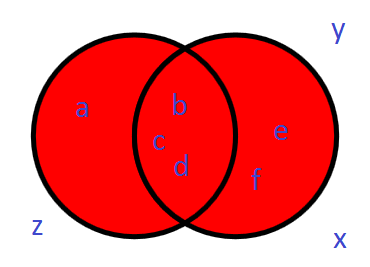
\includegraphics{sets-union.png}
\begin{figure}
\centering
\def\seta{(-1,0) circle (2)}
\def\setb{(1,0) circle (2)}
\begin{tikzpicture}
     \tikzstyle{element}=[minimum size=1mm, font=\large]
    \draw [fill=red]   \seta;
    \draw [fill=yellow]\setb;
    \begin{scope}[even odd rule]
        \clip \seta;
        \fill[fill=orange] \setb;
    \end{scope}
    \draw \seta;
    \draw \setb;
    \foreach \t/\x/\y in { z/-3/-2, x/3/-2, y/3/2, a/-2/0, b/-.1/1, c/.3/0, d/-.2/-1,
    e/2/.5, f/1.5/-.5 }
        \node[element] (\t) at (\x,\y) {$\t$};
\end{tikzpicture}
\caption{Пересечение двух множеств}
\end{figure}


Здесь $x$, $y$ и $z$ — это просто некоторые элементы, которые не вошли ни в одно из множеств. Всегда при работе со множествами (да и вообще всегда) важно рассматривать не только объекты, с которыми мы непосредственно работаем, но и внешние факторы. Красным цветом обозначено объединение двух множеств, представляемых кругами.

{\bfseries Определение.} Пересечением множеств $A$ и $B$ ($A\cap B$) называется множество, которое содержит лишь те элементы которые принадлежат сразу обоим множествам: $\forall x, (x\in A \wedge x \in B \leftrightarrow x\in A\cap B)$.

{\bfseries Пример.} Пусть $A = \{a, b, c, d\}$ и $B = \{b, c, d, e, f\}$. Тогда $A\cap B = \{b, c, d\}$

{\bfseries Упражнение.} Нарисуйте круги Эйлера для пересечения множеств (какую часть рисунка надо закрасить цветом?)

{\bfseries Определение.} Множества называются {\slshape непересекающимися}, если $A\cap B = \emptyset$ (то есть множества не имеют общих элементов). В противном случае множества называются пересекающимися.

{\bfseries Пример.} Множества $\{a, b, c\}$ и $\{d, e, f\}$ не пересекаются. Множества $\{a, b\}$ и $\{b, c\}$ пересекаются, и их пересечением является множество $\{b\}$.

{\bfseries Определение.} Разностью множеств $A\setminus B$ называется множество, содержащее все те элементы $A$, которые не содержатся в $B$: $\forall x, (x \in A\cap B \leftrightarrow x\in A \wedge x \not \in B)$.

{\bfseries Пример.} Пусть $A = \{a, b, c, d\}$ и $B = \{b, c, d, e, f\}$. Тогда $A\setminus B = \{a\}$

{\bfseries Упражнение.} Нарисуйте круги Эйлера для разности множеств.

{\bfseries Определение.} {\slshape Симметрической разностью} множеств $A\bigtriangleup B$ называется множество $(A\setminus B)\cup (B\setminus A)$, то есть множество элементов, принадлежащих либо $A$, либо $B$, но не их пересечению: $\forall x,(x\in A\bigtriangleup B \leftrightarrow x\in A \oplus x\in B)$.

{\bfseries Пример.} Пусть $A = \{a, b, c, d\}$ и $B = \{b, c, d, e, f\}$. Тогда $A\bigtriangleup B = \{a, e, f\}$.

{\bfseries Упражнение.} Нарисуйте круги Эйлера для симметрической разности множеств.

Часто при работе со множествами, мы держим в уме, что все элементы нашего множества являются элементами некоторого другого более крупного множества, содержащего все возможные объекты рассматриваемой нами задачи. Например, если мы говорим о множестве звёзд на небе, то мы можем держать в уме так же множество всех звезд вообще, а не только видимых нам. Если мы говорим о множестве учеников десятого класса школы N469, то как более общее множество мы можем подразумевать множество вообще всех учеников этой школы, либо же множество всех школьников страны, либо же множество всех людей. Смотря что за задачу мы решаем. Поэтому оказывается полезным ввести следующее определение:

{\bfseries Определение.} {\slshape Универсальным множеством}, или {\slshape универсумом}, называется множество всех возможных элементов, имеющих смысл в решаемой задаче.

{\bfseries Пример.} Если посмотреть на круги Эйлера, приведенные выше для иллюстрации объединения множеств и считать, что на картинке представлены все интересные нам элементы, то там универсумом в этом случае является множество $U = \{a, b, c, d, e, f, x, y, z\}$.

{\bfseries Определение.} {\slshape Дополнением} множества $A$ (обозначается как $A^C$) называется множество элементов универсума, не принадлежащих множеству $A$: $\forall x, x\in A^C \leftrightarrow x\in U \wedge x \not \in A$, где $U$ — универсум. Это же можно записать и без упоминания универсума, если предположить, что мы держим его «в уме»: $\forall x, x\in A^C \leftrightarrow x\not \in A$.

Понятно, что для операции дополнения необходимо строгое задание универсума, иначе она теряет смысл.

{\bfseries Пример.} Пусть $U = \{a, b, c, d, e, f, x, y, z\}$ и $A = \{a, b, c, d\}$. Тогда $A^C = \{e, f, x, y, z\}$.

{\bfseries Упражнение.} Нарисуйте круги Эйлера для дополнения.

Основные понятия мы определили, теперь надо разобраться с их свойствами. Однако прежде чем мы сформулируем нашу первую теорему о множествах, сделаем такое существенное наблюдение: практически все логические операции и операции над множествами находятся в соответствии друг с другом и операции над множествами определяются просто через логические операции. Так, логическое И задает пересечение множеств. Логическое ИЛИ — объединение. Исключающее ИЛИ — симметрическую разность. Отрицание высказываний — дополнение множеств. Эквиваленция — равенство множеств. Импликация — подмножества. В некотором смысле можно так же провести аналогию между универсумом и истинным высказыванием, а так же пустым множеством и ложным высказыванием.

Для продвинутых читателей, которые целиком осилили и поняли первую главу, отмечу, что сильно извратившись (как раз как я люблю), определить можно не только операции над множествами через операции над высказываниями, но и наоборот. Пусть, например, у нас есть теория $T_0$ и формулы $\phi$ и $\psi$. Пусть у нас так же есть теория $T_1$, для которой известно, что $\mathrm{Mod}(T_1) = \mathrm{Mod}(T_0, \phi) \cup \mathrm{Mod}(T_0, \psi)$. Тогда можно показать (сделайте это самостоятельно), что теория $T_1 = T_0 \cup \{\phi\vee \psi\}$ будет иметь как раз требуемое множество моделей (хотя такая теория может быть конечно не единственна), и именно через свойства моделей при добавлении формул можно определить логическое ИЛИ. Нечто аналогичное мы делали, когда определяли понятие импликации. Нечто аналогичное можно сделать и для всех других логических операций.

{\bfseries Теорема 1}. Для операций над множествами справедливы следующие законы:

{\slshape Ассоциативность:}

1) $(A \cap B) \cap C = A \cap (B \cap C)$

2) $(A \cup B) \cup C = A \cup (B \cup C)$

3) $(A \bigtriangleup B) \bigtriangleup C = A \bigtriangleup (B \bigtriangleup C)$

{\slshape Коммутативность:}

4) $A \cap B = B \cap A$

5) $A \cup B = B \cup A$

6) $A \bigtriangleup B = B \bigtriangleup A$

7) $A = B$ равносильно $B = A$.

{\slshape Дистрибутивность:}

8) $A \cap (B \cup C) = (A \cap B) \cup (A \cap C)$

9) $A \cup (B \cap C) = (A \cup B) \cap (A \cup C)$

10) $A \cap (B \bigtriangleup C) = (A \cap B) \bigtriangleup (A \cap C)$

{\slshape Двойное дополнение:}

11) $(A^C)^C = A$

{\slshape Законы де Моргана:}

12) $(A \cap B)^C = A^C \cup B^C$

13) $(A \cup B)^C =A^C \cap B^C$

{\slshape Еще по мелочам (здесь $U$ — универсальное множество):}

14) $A \cap U = A$

15) $A \cap \emptyset = \emptyset$

16) $A \cup U = U$

17) $A \cup \emptyset = A$

18) $A \bigtriangleup \emptyset = A$

19) $A \bigtriangleup U = A^C$

20) $A \cap A^C = \emptyset$

21) $A \cup A^C = U$

22) $A \bigtriangleup A^C = U$

23) $A\cap A = A$

24) $A\cup A = A$

25) $A \bigtriangleup A = \emptyset$

26) $A \cap (A^C \cup B) = A \cap B$

27) $A \cup (A^C \cap B) = A \cup B$

{\slshape Новенькое для отрицания:}

28) $A \setminus B = A \cap B^C$

{\slshape Свойства подмножеств:}

29) Если $A \not \subset B$, то $A$ и $B^C$ пересекаются.

30) $A \subset A$

31) Транзитивность: $A \subset B \wedge B \subset C \rightarrow A \subset C$ (думаю на всякий случай это свойство полезно проговорить словами: если $A\subset B$ и $B\subset C$, то $A\subset C$)

32) $A \subset B\cap C \rightarrow A \subset B$

33) Если $A \subset B$, то $B^C \subset A^C$ и наоборот.

{\bfseries Доказательство.} Во-первых, как можно заметить, все эти свойства дублируют соответствующие свойства для логических операций. Такой вот поворот событий. Некоторые свойства пришлось немного переформулировать (в основном в части с импликацией), одно свойство добавилось для разности множеств, несколько свойств потеряли смысл в теории множеств либо стали неинтересны. Но в целом мы имеем то же самое один в один.

Доказательства всех этих свойств оказываются совершенно элементарны и сводятся, как можно догадаться, к простой переформулировке на языке логики. Давайте докажем, например свойство 10 (мы здесь активно используем задание подмножеств предикатами, которые в нашем случае являются простой логической формулой, а так же дистрибутивность из теоремы 1 главы 1):

$A \cap (B \bigtriangleup C) = \{x|x\in A \wedge x \in B\bigtriangleup C\} = \{x|x\in A \wedge (x \in B \oplus x \in C)\}\\ = \{x|(x\in A \wedge x \in B) \oplus (x \in A \wedge x \in C)\} = \{x|(x\in A \cap B) \oplus (x \in A \cap C)\} \\ = \{x|x\in (A \cap B) \bigtriangleup (A \cap C)\} = (A \cap B) \bigtriangleup (A \cap C)$

Что и требовалось. Как видно из этих рассуждений, операции над множествами и операции над высказываниями — это действительно очень близкие понятия, которые во многом отражают одно и то же, только несколько под разным углом.

Остальные свойства докажите самостоятельно в качестве упражнения, а так же нарисуйте круги Эйлера для этих свойств — они должны дать довольно не плохую интуицию относительно свойств множеств (и заодно логики). \qed

В завершение параграфа определим еще одну операцию, которая уже не имеет никакого прообраза в логике.

{\bfseries Определение.} {\slshape Булеаном} множества $A$ (обозначается $2^A$) называется множество всех его подмножеств.

{\bfseries Пример.} Пусть $A = \{a, b, c\}$. Тогда $2^A = \{\emptyset, \{a\}, \{b\}, \{c\}, \{a, b\}, \{a, c\}, \{b, c\}, A\}$.

Обратите внимание, что всегда $\emptyset \in 2^A$ и $A\in 2^A$. Так же обратите внимание на то, что булеан, сам являясь множеством, содержит в качестве своих элементов другие множества (это ничему не противоречит — элементами множеств могут быть и другие множества, почему бы и нет?).

Так же важно отметить такой нюанс: если $a \in A$, то $\{a\} \in 2^A$, но $a \not \in 2^A$. Это довольно очевидно: $a\not = \{a\}$, ведь множество состоящее из одного элемента и сам этот элемент логически разные сущности.

Понятие булеана будет активно использоваться нами в дальнейшем, а пока мы рассмотрим опять же аналогию булеана с логикой (это только для дотошных читателей). Пусть $A$ — некоторое одноэлементное множество. Тогда $2^A = \{\emptyset, A\}$.Теперь, если рассматривать наши операции над множествами, ограничившись лишь этим булеаном, то если назвать $\emptyset$ ложью, а $A$ истиной, то наша аналогия между логическими операциями и операциями над множествами станет уже не примерной, а совершенно однозначной.

Таким образом можно считать, что логика — это в некотором смысле частный случай теории множеств, которая в свою очередь является обобщением логики. Если рассматривать $A$, который состоит из многих элементов, то можно в некотором смысле говорить, что $2^A$ — это модель нечеткой логики, где $A$ — истинное высказывание, $\emptyset$ — ложное высказывание, а остальные множества являются истинными высказываниями лишь с некоторой степенью вероятности. Это далеко не самый удобный подход для определения нечеткой логики, и на практике математиками не используется наверное никогда, кроме очень узких областей, однако мы будем иногда обращаться к этому примеру в качестве иллюстраций и более интуитивного понимания отдельных понятий.

Так же у дотошного читателя может возникнуть определенный дискомфорт от той последовательности изложения, которую он до сих пор наблюдает: говоря о логике и предикатах мы ввели понятие множеств, говоря о множествах мы во всю опирались на логигу. Это как в России: чтобы получить работу по специальности, надо иметь опыт работы по этой специальности, а чтобы получить опыт, надо проработать по этой специальности. Такие ситуации допустимы в быту, но не в науке, поэтому порочные круги необходимо разрывать.

Пока я стараюсь дать просто интуицию о множествах, поскольку строгое формальное изложение без порочных кругов и без начальной интуиции вряд ли окажется сильно полезно и понятно читателю. Поэтому пока мы оставим все как есть, а формальное изложение проведем в конце главы, где уже окончательно расставим все на свои места и избавимся от всех неточностей и нечеткости в определениях.

\section{Отношения}

{\bfseries Определение.} {\slshape Упорядоченным набором}, или же {\slshape кортежем}, или же {\slshape отношением}, называется набор объектов, в котором так же определен порядок этих объектов.

Как обычно это совершенно чудовищное определение, которое не может считаться строгим математическим, но пока мы попробуем работать с ним, напирая на интуицию, а не научную строгость. Записывается упорядоченный набор как $(a, b, \ldots, z)$, где элементы $a$, $b$ и $z$ являются элементами некоторых определенных множеств.

Как более-менее практический пример можно рассмотреть базы данных. Чтобы не говорить слишком абстрактно, а рассмотреть более конкретную ситуацию, можно рассмотреть простую записную книжку мобильного телефона, которая тоже по сути является компьютерной базой данных.

Сама база данных представляет из себя множество записей, каждая из которых состоит из нескольких полей. Это можно представить как таблицу:

\begin{table}[h]
\begin{tabular}{lllll}
Фамилия & Имя & Телефон & ДР & Комментарий\\
Авраам & Линкольн & +1(270)... & 12.02.1802 & Президент\\
Бенито & Муссолини & +3(39)... & 29.07.1883 & Фашик\\
Владимир & Ленин & +7(499)... & 22.04.1870 & Свой мужик\\
Григорий & Распутин & +7(3459)... & 21.01.1869 & Есть чему завидовать\\
Джорджина & Байер & +6(64)... & 11.1957 & Транссексуал\\
... & ... & ... & ... & ...
\end{tabular}
\end{table}

Если предположить, что $F$ — множество фамилий, $N$ — множество имен, $P$ — множество телефонов, $D$ — множество дат календаря и $S$ — множество произвольных текстовых строк, то можно сказать, что данная таблица иллюстрирует множество упорядоченных наборов следующего вида:

$\{(f, n, p, b, c)|f\in F, n \in N, p \in P, b \in D, c \in S\}$

(Строго говоря с точки зрения логики правильнее было бы писать не символ запятой справа в предикате, а символ $\wedge$, но чаще в случаях, подобных нашему, употребляется именно запятая в силу большей наглядности и удобства — означает она при этом логическое И).

Практически вся теория баз данных построена на самом деле на теории множеств в рамках того, что я уже рассказал, и декартова произведения, о котором речь пойдет ниже. База данных — это множество, элементами которого являются упорядоченные наборы. Команды работы с базой данных — это операции, задающие предикаты и операции над множествами. Я не могу позволить себе углубляться сейчас в алгебру реляционных баз данных и синтаксис языка SQL, но вообще рекомендую всем читателям с этими вещами ознакомиться — будет небесполезно, а заодно увидите кучу примеров тому, о чем я сейчас говорю.

Здесь стоит еще сделать такое наблюдение по терминологии. Чаще всего термин кортеж применяется именно в теории баз данных, термин отношение применяется чаще всего в случае упорядоченных пар, в которых оба элемента принадлежат одному и тому же множеству $\{(x, y)|x\in A, y\in A\}$, а термин упорядоченный набор используется в остальных случаях. Здесь нет строгого формального разграничения, это просто сложившаяся практика, которая однако может часто нарушаться и в этом нет ничего преступного.

{\bfseries Определение.} {\slshape Декартовым}, или {\slshape прямым}, {\slshape произведением} множеств $A$ и $B$ называется множество $A\times B = \{(a, b)|a\in A, b\in B\}$.

Говоря человеческим языком, $A\times B$ — это множество всех возможных упорядоченных пар $(a, b)$, таких что $a\in A$ и $b \in B$.

{\bfseries Пример.} Пусть $A = \{0, 1\}$, а $B = \{a, b, c\}$. Тогда $A\times B = \{(0, a), (0, b), (0, c), (1, a), (1, b), (1, c)\}$.

Кое-какую интуицию относительно декартова произведения вероятно поможет развить иллюстрация в виде таблицы. Столбцы в ней отводятся для элементов одного множества, строки — для другого множества, а на пересечении стоит их декартово произведение:

$\begin{array}{c|ccc}\times & a&b&c\\ \hline 0 & (0,a) & (0, b) & (0, c) \\ 1 & (1, a)& (1, b) &(1, c)\end{array}$

{\bfseries Пример.} Часто с помощью декартова произведения можно описывать какие-то физические понятия. Пусть $A$ — множество мастей (червы, буби, крести, трефы), а $B$ — множество достоинств (6, 7, 8, ..., король, туз). Тогда $A \times B$ — множество игральных карт в колоде.

{\bfseries Упражнение.} Покажите, что в общем случае $A\times B \not = B \times A$. В каких частных случаях все же $A\times B = B \times A$?

Легко заметить, что $(A\times B)\times C \not= A\times (B \times C)$, поскольку в случае множества до знака равенства будут получаться пары вида $((a, b), c)$, а для множества справа от знака равенства будут пары $(a, (b, c))$. Однако как и раньше удобно считать, что произведение $A\times B\times C$ без скобок дает нам упорядоченные тройки $(a, b, c)$ так же без каких-либо специальных группировок. Для удобства часто, впрочем, считают, что и при наличии скобок декартово произведение дает обычные упорядоченные наборы: $(A\times B)\times C = \{(a, b, c)|a\in A, b\in B, c\in C\}$.

Каждое отношение таким образом является подмножеством декартова произведения $\rho \subset X\times X$ — в этом параграфе нас будут интересовать как раз такие отношения. Часто для удобства применяется так же следующая запись: если $(x, y) \in \rho$, то пишут $x\rho y$. Из последующего текста будет видно почему это удобно.

{\bfseries Пример.} Пусть $S$ — множество высказываний. Тогда любая логическая операция задает отношение на этом множестве. В простейшем случае, если рассматривать только одно истинное и ложное высказывание $S = \{0, 1\}$, то $\vee = \{(1, 0), (0, 1), (1, 1)\}$, $\leftrightarrow = \{(0, 0), (1, 1)\}$ и так далее. По аналогии любому предикату на множествах можно сопоставить в соответствие некоторое отношение (возможно, не из двух элементов).

{\bfseries Определение.} Отношение называется {\slshape рефлексивным}, если для любого $x$ выполняется $x\rho x$.

{\bfseries Определение.} Отношение называется {\slshape антирефлексивным}, если для любого $x$ отношение $x\rho x$ не имеет места быть.

{\bfseries Определение.} Отношение называется {\slshape транзитивным}, если для любых $x$, $y$ и $z$ из того, что $x\rho y$ и $y \rho z$ следует, что $x\rho z$.

{\bfseries Определение.} Отношение называется {\slshape симметричным}, если из того, что $x\rho y$ следует $y\rho x$.

{\bfseries Определение.} Отношение называется {\slshape антисимметричным}, если из того, что $x \rho y$ и $y \rho x$ следует, что $x = y$.

Можно привести и больше возможных общих свойств отношений, но для наших нужд достаточно и того что я уже привел.

{\bfseries Упражнение.} Запишите эти свойства на языке логики.

{\bfseries Упражнение}. Приведите пример нетранзитивного отношения на множестве $\{0, 1\}$.

{\bfseries Определение.} Отношение называется {\slshape отношением эквивалентности}, если оно рефлексивно, транзитивно и симметрично.

Отношение эквивалентности часто обозначается символами $=$, $\approx$, $\sim$ и подобными (хотя есть и другие обозначения, которые мы будем по ситуации использовать). Если на множестве задано несколько отношений эквивалентности, то символьное обозначение отношения часто указывается справа внизу от знака эквивалентности: $\approx_R$.

{\bfseries Упражнение.} Пусть $S$ — множество учеников средней школы №469. Отношение $x\approx_Y y$ означает, что ученики $x$ и $y$ заканчивают школу в одном году, отношение $x \approx_C y$ означает, что они учатся в одном классе, $x \sim y$ что имеют одинаковую успеваемость. Проверьте, что все заданные отношения — это отношения эквивалентности (для этого необходимо проверить, что они рефлексивны, транзитивны и симметричны).

Следующие три упражнения уже посложнее, и их начинающие могут пропустить.

{\bfseries Упражнение.} Пусть $S$ — некоторое множество, а $P$ — множество предикатов, определенных на этом множестве. Пусть нам задано такое отношение, что $p \approx q$ тогда и только тогда, когда $p$ и $q$ определяют одинаковые подмножества $S$. Докажите, что это отношение эквивалентности.

{\bfseries Упражнение.} Пусть нам задано множество логических формул, все с одинаковым числом параметров. Отношение $f=g$ определено для функций, которые на одинаковых значениях параметров принимают одинаковые значения истинности. Докажите, что это отношение эквивалентности.

{\bfseries Упражнение.} Пусть нам задана некоторая теория. Докажите, что семантическая эквивалентность формул является отношением эквивалентности. (Напомню, что формулы $\phi$ и $\psi$ семантически эквивалентны, если в любой модели теории $\psi\leftrightarrow\phi$).

Примеры, приведенные в упражнении, демонстрируют основную идею отношения эквивалентности: это набор пар, которые имеют какие-то общие характеристики, которые и отражают отношение. Причем мыслить об отношении как о парах элементов чаще всего не удобно с интуитивной точки зрения — удобнее мыслить об отношении эквивалентности именно как о наличии какого-то общего свойства.

{\bfseries Определение.} Пусть дано множество $A$ и на нем задано отношение эквивалентности $\sim$. Множество всех элементов $x$, для которых $a\sim x$ называется {\slshape классом эквивалентности} элемента $a$ и обозначается как $[a]$.

{\bfseries Теорема.} Для любых элементов $a, b \in A$ классы эквивалентности $[a]$ и $[b]$ либо совпадают, либо не пересекаются.

{\bfseries Доказательство.} Проведем доказательство от противного и предположим, что теорема неверна. Пусть классы эквивалентности $[a]$ и $[b]$ пересекаются, но не совпадают. Тогда найдется элемент $x$, принадлежащий сразу обоим классам эквивалентности, и элемент $b' \in [b]$, такой что $b' \not\in [a]$. Для него однако верно, что $b' \sim x$, но поскольку $x \in [a]$ и $x\sim a$, то в силу транзитивности $b' \sim a$ и соответственно $b' \in [a]$. Полученное противоречие говорит, что наше предположение «от противного» было не верно, и значит теорема верна. \qed

Это доказательство на первый взгляд может показаться странным и непонятным — вспомните тогда свойства импликации $(a\rightarrow b) \leftrightarrow (\neg b \rightarrow \neg a)$ и как она связана с выводимостью (см. §1.6).

Смыслом теоремы является тот факт, что каждое множество с заданным на нем отношением эквивалентности можно разбить на непересекающиеся классы эквивалентности.

{\bfseries Пример.} Пусть опять $S$ — множество учеников школы №469. Всех учеников можно сгруппировать по классам, по успеваемости или по году окончания школы. Пусть $A$ — множество двоечников, $B$ — троечников, $C$ — хорошистов и $D$ — отличников. Очевидно, что эти множества не пересекаются и $S = A\cup B\cup C\cup D$, причем любые два ученика из одного и того же множества находятся в отношении $\sim$ («имеют одинаковую успеваемость») друг с другом, а ученики из разных множеств в этом отношении не находятся.

{\bfseries Определение.} Процесс разбиения множества на классы эквивалентности называется {\slshape факторизацией}, а само множество классов эквивалентности называется {\slshape фактор-множеством}. Если $\rho$ — отношение эквивалетности на $A$, то фактормножество $A$ по $\rho$ обозначается как $A/\rho$.

{\bfseries Пример.} Продолжая пример с успеваемостью, можно записать, что $S/\sim = \{A, B, C, D\}$.

Обратите внимание в какую сторону рисуется черта фактормножества и не путайте ее с разностью множеств. $A\setminus B$ — разность, а $A/\rho$ — факторизация.

Интуитивно таким образом можно рассматривать факторизацию как разбиение множества на подмножества в соответствии с некоторым отношением («фактором»). Обратное кстати тоже верно — если множество разбито на непересекающиеся подмножества, то по ним можно задать отношение эквивалентности.

{\bfseries Упражнение.} Пусть $A = \{a, b, c, d\}$ разбито на подмножества $\{a, b\}$ и $\{c, d\}$. Запишите по этому разбиению отношение эквивалентности $\rho$ как множество упорядоченных пар (начинается эта запись как $\rho = \{(a, a), (a, b), \ldots\}$).

Перейдем теперь ко второму не менее важному отношению, которое мы сравнительно часто будем использовать.

{\bfseries Определение.} Отношение называется {\slshape отношением частичного порядка} (или {\slshape отношением нестрогого частичного порядка}), если оно рефлексивно, транзитивно и антисимметрично.

{\bfseries Определение.} Отношение называется {\slshape отношением строгого частичного порядка}, если оно антирефлексивно, транзитивно и антисимметрично.

Отношение частичного порядка удобно обозначать как $\le$. Отношение строго частичного порядка как $<$. Если $a \le b$ и $a \not= b$, то $a<b$. Если $b \le a$, то можно писать $a \ge b$ или $a > b$, если $a\not= b$. Легко видеть, что отношения частичного и строгого частичного порядка — это фактически одного и то же. Различаются они лишь тем, находится ли каждый элемент в отношении с самим собой (то есть можем ли мы записать отношение $x\le x$). В теории в основном используется отношение частичного порядка, в конкретных задачах часто может оказаться удобным и то и другое. Хотя погоды это разграничение не делает: если у нас есть строгий порядок, то его всегда можно сделать не строгим, дополнив парами $x\le x$, и наоборот нестрогий порядок можно сделать строгим, выкинув такие пары.

{\bfseries Упражнение.} Докажите, что если элементами множества являются множества (например, это булеан), то отношение $\subset$ является отношением частичного порядка.

{\bfseries Упражнение.} Докажите, что отношение «является предком» на множестве людей является строгим частичным порядком.

{\bfseries  Упражнение.} Докажите, что отношение «не ниже чем» на множестве всех людей образует нестрогий частичный порядок, а отношение «выше чем» строгий частичный порядок.

{\bfseries Упражнение.} Покажите, что отношение «является родителем» не является отношением частичного порядка.

{\bfseries Упражнение.} Покажите, что на множестве картонных коробок отношение «влезает в» является отношением строгого частичного порядка.

{\bfseries Упражнение.} Рассмотрим множество всех логических функций с одинаковым числом параметров. Определим на них отношение следующим образом: $f\le g$ тогда и только тогда, когда на одинаковых наборах параметров либо эти функции принимают одинаковое значение, либо $f=0$, а $g=1$. Докажите, что отношение частичного порядка. Как оно соотносится с порядком на булеане множества?

{\bfseries Пример.} В микроэкономике рассматриваются отношения предпочтений, задаваемые на множествах альтернатив (читай товаров). Считается, что потребители могут сравнивать альтернативы по степени предпочтительности и данное отношение является как раз отношением частичного порядка. (Психологи однако доказывают, что предпочтения людей не являются рациональными и таким образом не образуют частичный порядок на множестве товаров).

Отношение частичного порядка удобно представлять в виде диаграмм. Например, так будет выглядеть диаграмма для булеана множества $\{x, y, z\}$:

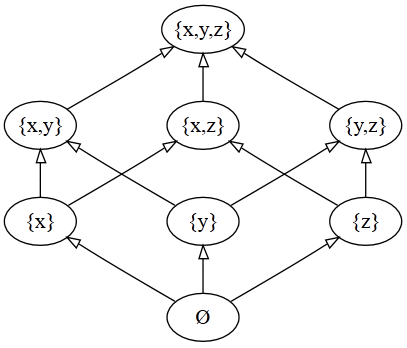
\includegraphics{hasse1.png}

(Картинка из Википедии, свободной энциклопедии, потому что сам не умею пока такие рисовать; LibreOffice Draw не справляется с задачей).

Здесь стрелка обозначает отношение «является подмножеством». Элементы, располагающиеся выше, оказываются «больше» элементов, располагающихся внизу, если между ними есть путь из стрелок. Если на диаграмме есть стрелка $a\to b$ и стрелка $b\to c$, то по транзитивности должна быть и стрелка $a\to c$, которая не указывается, чтобы не загромождать картинку.

Отношение частичного порядка таким образом упорядочивает элементы множества. Существенно, однако, что если задан частичный порядок, то совершенно не факт, что удастся сравнить произвольные два объекта. Как видно из диаграммы выше, элементы $\{x, y\}$ и $\{z\}$ не сравнимы между собой. Точно так же для любых двух людей не обязательно кто-то один из них должен быть предком другого, и в этом смысле не сравнимыми являются брат и сестра.

{\bfseries Определение.} {\slshape Линейным порядком} называется отношение частичного порядка, относительно которого сравнимы любые два элемента множества.

{\bfseries Пример.} Отношение «не ниже чем» является линейным порядком на множестве людей.

{\bfseries Определение.} {\slshape Максимальным элементом} называется такой элемент, что не существует элемента, большего него.

{\bfseries Определение.} {\slshape Наибольшим элементом} называется такой элемент, что он больше любого другого элемента.

{\bfseries Пример.} На множестве коробок максимальным элементом будет коробка, которая не может влезть ни в какую другую коробку. Наибольшим элементом будет коробка, в которую может поместиться любая другая коробка.

В полной аналогии можно ввести понятия {\slshape минимального} и {\slshape наименьшего элемента}, но мы не будем на это отвлекаться, так там вся теория совершенно аналогична.

Очевидно, что если множество обладает наибольшим элементом, то он же будет и единственным максимальным элементом. Однако же максимальных элементов может быть несколько, и наибольшего элемента в этом случае не будет, как в случае следующей диаграммы:

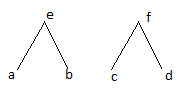
\includegraphics{maxelement.png}

(На этот раз рисовал сам; извиняюсь за качество — я математик, а не художник; я когда-нибудь научусь и переделаю это убожество).

На приведенной диаграмме два максимальных элемента: $e$ и $f$. Наибольшего элемента нет. На следующей же диаграмме уже имеется один наибольший элемент $g$, он же является и максимальным:

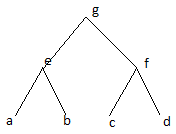
\includegraphics{hielement.png}

(Я правда надеюсь, что мне кто-нибудь из читателей поможет с иллюстрациями).

В обоих этих примерах порядки не являлись линейными. В случае же линейного порядка, очевидно, что понятия максимального и наибольшего элемента совпадают.

{\bfseries Определение.} {\slshape Верхней гранью} подмножества $S\subset U$ называется такой элемент $x\in U$, что для любого элемента $s\in S$ выполняется $s \le x$.

{\bfseries Определение.} {\slshape Нижней гранью} подмножества $S\subset U$ называется такой элемент $x\in U$, что для любого элемента $s\in S$ выполняется $s \ge x$.

Если $x$ — верхняя грань подмножества $S$, то любой элемент больший $x$ так же будет являться верхней гранью $S$. Таким образом, верхние грани сами по себе образуют множество (аналогично с нижними) и есть смысл ввести следующие определения:

{\bfseries Определение.} {\slshape Наименьшей}, или {\slshape точной}, {\slshape верхней гранью}, называется наименьшая из верхних граней. Обозначается она как $\sup S$.

{\bfseries Определение.} {\slshape Наибольшей}, или {\slshape точной}, {\slshape нижней гранью}, называется наибольшая из нижних граней. Обозначается она как $\inf S$.

(С этого места начинаются абстракции, которые начинающему читателю вероятно и не являются необходимыми — если будет не понятно о чем речь, можно смело пропускать. Если однако разобраться с материалом, то это будет хорошим упражнением для ума.)

Если подмножество $S$ состоит лишь из двух элементов, то операции «точных граней» можно рассматривать как арифметические операции над этими элементами. В этом случае используется запись $\sup\{a, b\} = a\vee b$ и $\inf\{a, b\} = a\wedge b$.

{\bfseries Упражнение.} Докажите, что на булеане относительно порядка, образованного включением множеств, $A\wedge B = A\cap B$ и $A\vee B = A \cup B$ и они обладают соответственно всеми свойствами логического И и логического ИЛИ.

Сформулированное в упражнении утверждение в общем случае неверно, если рассматривать произвольный частичный порядок. Во-первых, могут не выполняться сами свойства логических операций, а во-вторых самих точных граней может и не быть. Поэтому вводятся следующие определения:

{\bfseries Определение.} {\slshape Решёткой} называется частично упорядоченное множество, у которого для любого двухэлементного подмножества существуют точные верхние и нижние грани.

{\bfseries Определение.} {\slshape Дистрибутивной решёткой} называется решётка, для которой оказываются верны свойства дистрибутивности операций $\wedge$ и $\vee$ (см §1.1, теорема 1).

{\bfseries Упражнение.} Докажите, что решётка, изображенная на диаграмме ниже, не является дистрибутивной:

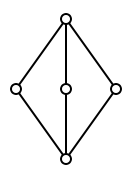
\includegraphics{lattice.png}

Дистрибутивные решетки уже практически дублируют законы логики, которым была посвящена первая глава. Не достает только $1$ и $0$. Следующие определения исправляют ситуацию:

{\bfseries Определение.} Решетка называется ограниченной, если в ней существуют наибольший и наименьший элементы, обозначаемые соответственно как $0$ и $1$.

{\bfseries Упражнение.} Если решетка имеет минимальный или максимальный элементы, то они будут единственны и будут являться наименьшим и наибольшим элементами. Докажите это.

{\bfseries Определение.} {\slshape Дополнением} элемента $x$ ограниченной решетки такой элемент $y$, что $x\wedge y = 0$ и $x \vee y = 1$. Дополение $x$ обозначается как $\neg x$.

{\bfseries Определение.} Если в решетке каждый элемент обладает дополнением, то такая решетка называется {\slshape решеткой с дополнением}.

{\bfseries Определение.} {\slshape Булевой алгеброй} называется дистрибутивная решетка, обладающая наименьшим и наибольшим элементами (обозначаемыми соответственно $0$ и $1$).

{\bfseries Пример.} Если рассмотреть двухэлементное множество $\{0, 1\}$ и определить на нем порядок $0 < 1$, то мы получим в точности классическую логику, которую рассматривали в первой главе, которая как теперь видно является разновидностью булевой алгебры.

{\bfseries Пример.} Булеан любого множества $A$ задает булеву алгебру относительно включения множеств, где наибольшим элементом является само множество $A$, а наименьшим пустое множество.

{\bfseries Упражнение.} Для булевых алгебр справедливы все законы логики, которые мы приводили в теореме 1.1. Докажите это.

Если у нас есть два частично упорядоченных множества $A$ и $B$, то на их декартовом произведении можно задать частичный порядок несколькими способами:

{\bfseries Определение.} {\slshape Лексигографическим порядком} на $A\times B$ называется порядок, при котором $(a, b) \le (a', b')$ либо когда $a < a'$, либо когда $a=a'$ и $b\le b'$.

{\bfseries Определение.} {\slshape Естественным порядком} на $A\times B$ называется порядок, при котором $(a, b) \le (a', b')$ тогда и только тогда, когда одновременно $a \le a'$ и $b \le b'$.

Оба этих порядка естественно распространяются на декартово произведение любого количества множеств.

{\bfseries Упражнение.} Пусть $B = \{0, 1\}$ и на нем введен порядок $0 < 1$. Будем рассматривать множество $B\times B\times \ldots \times B$ (фактически упорядоченные наборы единиц и нулей) с естественным частичным порядком. Докажите, что такой частичный порядок задает булеву алгебру (кстати, как раз ту самую, которая повсеместно используется в программировании и называется там побитовыми логическими операциями).

{\bfseries Упражнение.} Докажите, что линейно-упорядоченное множество является дистрибутивной решеткой, и соответственно при наличии наименьшего и наибольшего элемента является булевой алгеброй.

{\bfseries Упражнение.} Является ли булевой алгеброй множество $B\times B \times \ldots \times B$, введенное выше, относительно лексикографического порядка?

{\bfseries Упражнение.} Пусть теперь $B$ — некоторая произвольная булева алгебра. Является ли булевой алгеброй $B\times B \times \ldots \times B$ относительно лексикографического порядка? А относительно естественного порядка?

\section{Графы}

Этот параграф не содержит каких-то очень важных для нашего курса сведений — он просто призван служить демонстрацией отдельных понятий, которые мы вводили. Всё, о чем мы говорили до сих пор, может показаться слишком абстрактным и не практичным на первый взгляд, и в этом параграфе я на примере двух задач, очень простой и очень сложной, а так же нестрогих геометрических ассоциаций, покажу, что на самом деле даже то, что я изложил до сих пор, может оказаться вполне полезным, если грамотно это применить. Материал, связанный со второй задачей и многомерной геометрией на самом деле очень жесткий (и одновременно с тем неформальный), так что при первом знакомстве его можно пропустить. (Я вообще не уверен, был ли я прав, это написав).

Если говорить неформально, то граф — это набор точек, называемых вершинами, некоторые из которых соединенны линиями, называемыми рёбрами. Графы бывают многих разновидностей, но нас пока будут интересовать простые графы и ориентированные графы (кратко орграфы), у которых каждое ребро записывается в виде стрелки и называется дугой.

Мы уже встречали графы в прошлом параграфе: диаграммы частично упорядоченных множеств как раз представляют собой орграфы. Графы и орграфы часто используются для описания многих предметов нашей жизни: карта дорог между городами является графом, где дороги — это ребра графа, а города — вершины. Графом является схема компьютерной сети: каждый компьютер в таком графе является вершиной, а кабель, соединяющий их в сеть, является ребром. Ориентированные графы применяются всякими там менеджерами для планирования всяких там задач: у них вершинами графов являются задачи, которые необходимо исполнить, а дугами показывается зависимость между задачами (если из задачи $A$ в задачу $B$ идет стрелочка, то выполнение задачи $B$ не может быть начато до окончания задачи $A$). Инженеры используют разновидности графов для представления электрических цепей. И так далее. Некоторые из этих задач мы будем рассматривать в дальнейшем (в основном в виде простых самостоятельных упражнений).

Важно ответить, что граф — это именно набор вершин и ребер, но не их представление на бумаге. Если изменить форму ребер или положение вершин, граф от этого не изменится, хотя визуально может выглядеть и сильно по-другому. Например, следующие три графа одинаковы (научно говорят изоморфны):

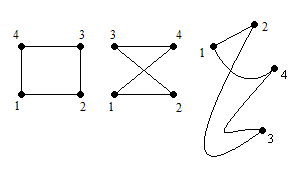
\includegraphics{isomorphic_graphs.png}

Что такое граф интуитивно, думаю, понятно. Давайте теперь все формализуем и определим графы через теорию множеств.

{\bfseries Определение.} {\slshape Графом} называется упорядоченная пара $(V, E)$, где $V$ — множество, элементы которого называются вершинами графа, а $E$ — симметричное антирефлексивное отношение на $V$, элементы которого называются ребрами графа.

{\bfseries Определение.} Если ослабить условия прошлого определения и разрешить, чтобы отношение $E$ не было симметричным, то такая конструкция будет называться {\slshape ориентированным графом}. Сами элементы множества $E$ называются в этом случае {\slshape дугами}.

Мы будем говорить преимущественно о неориентируемых графах. В общем случае антирефлексивность не требуется, но мы для простоты будем исключать из рассмотрения ребра вида $(a, a)$, чтобы не отвлекаться на различные частные случаи.

{\bfseries Определение.} Если $(v, w) \in E$, то вершины $v$ и $w$ называются {\slshape инцидентными}. Так же говорят, что $v$ и $w$ инцидентны ребру $(v, w)$, а ребро соответственно инцидентно его вершинам.

{\bfseries Упражнение.} Запишите отношения, соответствующие графам, изображенным выше, и убедитесь в том, что они действительно изоморфны.

Перейдем сразу к задачам. Первая из них простая и вполне себе классическая.

{\bfseries Задача.} Есть три дома и три колодца. Надо от каждого колодца к каждому дому провести тропинку. Возможно ли сделать это так, чтобы эти тропинки не пересекались?

Вот пример запоротого решения:

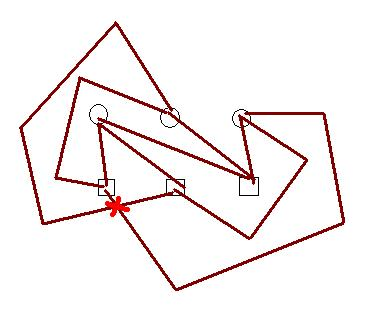
\includegraphics{bells.jpg}

Попробуйте вначале решить задачу самостоятельно, а потом читайте дальше.

{\bfseries Определение.} Граф, который возможно изобразить на плоскости без пересечения ребер, называется {\slshape планарным}.

Очевидно, что это ровно то, что нам требуется: надо проверить, является ли граф для домиков и колодцев планарным. Этот граф имеет специальное обозначение $K_{3, 3}$ и в простейшем виде, если не заморачиваться о пересечениях, может быть изображен так:

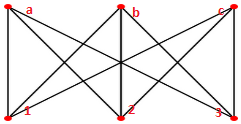
\includegraphics{k331.png}

Можно ли его нарисовать без пересечения линий? Для начала запишем его ребра в виде множества: $E = \{a1, a2, a3, b1, b2, b3, c1, c2, c3, \ldots\}$ Для удобства мы не стали перечислять симметричные отношения (понятно, что если $a1\in E$, то и $1a \in E$ и лишний раз упоминать это скучно) и ребра $(v, w)$ кратко записывали как $vw$.

{\bfseries Определение.} Граф $G' = (V', E')$ называется {\slshape подграфом} графа $G = (V, E)$, если $V' \subset V$ и $E' \subset E$.

Рассмотрим такое подмножество ребер: $C = \{a1, 1b, b2, 2c, c3, 3a\}$. Эти ребра образуют такой подграф:

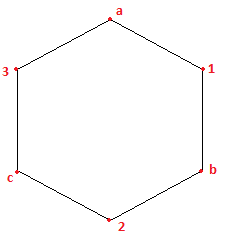
\includegraphics{cycle.png}

Подобные последовательности имеют специальные названия. Просто упомянем их для порядку:

{\bfseries Определение.} Последовательность чередующихся вершин и ребер, в которой каждое ребро стоит между различными вершинами, которым оно инцидентно, называется {\slshape путем}.

В нашем случае путь записывается как последовательность $a, a1, 1, 1b, b, b2, 2, 2c, c, c3, 3, 3a, a$.

{\bfseries Определение.} Если в пути нет повторяющихся ребер, то он называется {\slshape цепью}.

{\bfseries Определение.} Если первая и последняя вершины цепи совпадают, то такой путь называется {\slshape замкнутой цепью}, либо {\slshape циклом}. Если не совпадают, то цепь {\slshape незамкнута}.

Приведенный нами подграф $C$ очевидно является циклом и иллюстрация дает понять откуда берется такое называние. И хочешь не хочешь, но как этот цикл не рисуй он всегда либо будет иметь самопересечения, либо будет разбивать плоскость на две части: внутреннюю и внешнюю, и в этом смысле наш цикл имеет простейший вид какой только возможно (По хорошему это тоже надо строго доказывать да и вообще определять что значит «разбивает плоскость», но мы это сделаем намного позже, когда будем говорить о геометрии, а пока что просто доверимся интуиции).

Множество рёбер нашего первоначального графа $E = C \cup \{a2, b3, c1\}$ и нам необходимо дорисовать к подграфу $C$ три ребра, чтобы получить $E$. Здесь можно просто рассмотреть все возможные варианты. Если нарисовать $a2$ внутри цикла, то $b3$ и $c 1$ должны быть снаружи цикла, иначе они будут пересекать ребро $a2$. Но оба ребра $b3$ и $c 1$ тоже не могут быть одновременно снаружи, так как в этом случае они так же будут пересекаться. Значит, $a2$ не может быть нарисован внутри цикла так, чтобы граф $K_{3, 3}$ не имел пересечений. Однако если нарисовать $a2$ снаружи цикла, то так же можно увидеть, что $b3$ и $c 1$ неминуемо пересекутся внутри цикла. Таким образом мы перебрали все возможные варианты и убедились:

{\bfseries Лемма.} Граф $K_{3, 3}$ не является планарным.

Это ровно то что требовалось выяснить в условиях задачи.

Термин «лемма» обычно (но не всегда) используется для обозначения промежуточных результатов, которые будут задействованы далее в каких-то более сильных утверждениях. Самостоятельно предлагаю доказать вам еще следующую лемму:

{\bfseries Лемма.} Граф $K_5$ имеющий вершины $\{a, b, c, d, e\}$, каждая пара которых инцидентна, не планарен.

В простом виде этот граф выглядит так:

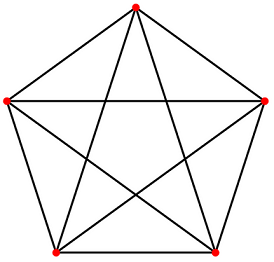
\includegraphics{k5.png}

Его не планарность доказывается так же, как и в случае с графом $K_{3, 3}$.

Из двух лемм, сформулированных выше, можно получить такую теорему:

{\bfseries Теорема.} Граф, который содержит в качестве подграфов $K_{3, 3}$ или $K_5$ не планарен.

Оказывается, что наличие подграфов, которые структурно схожи с $K_{3, 3}$ или $K_5$ является и необходимым условием. «Структурно схожи» можно выразить строго следующими терминами (в следующих определениях я опять не упоминаю симметричных отношений для краткости):

{\bfseries Определение.} Пусть дан граф $G=(V, E)$ и $(a, b) \in E$. Тогда {\slshape разбиением} графа $G$ по дуге $(a, b)$ называется граф $G' = (V\cup\{x\}, E\cup\{(a, x), (x, b)\}\setminus\{(a, b)\})$.

{\bfseries Определение.} Графы $A$ и $B$ называются {\slshape гомеоморфными}, если существует граф, такой что оба графа $A$ и $B$ получаются из него некоторыми разбиениеями дуг.

{\bfseries Теорема Куратовского.} Граф является планарным тогда и только тогда, когда он не содержит подграф, гомеоморфный $K_{3, 3}$ или $K_5$.

Разбиение графа — это вставка вершины посреди какого-то ребра. Эта операция, очевидно, не влияет на возможность нарисовать граф планарно: подразбиение это просто выделение точки на линии. Например, мы на каждой тропине от колодца к домику могли бы поставить опорный пункт полиции. Понятно, что граф уже не был бы равен $K_{3, 3}$, но в целом выглядел бы он точно так же.

Доказывать теорему Куратовского мы не будем, потому что я не знаю как ее доказывать, да и не особо она нужна по большому счету (в рамках этого курса точно не пригодится). Я когда сам в свое время начинал читать доказательство, мне оно показалось скучным и длинным, и я бросил это занятие. Если хотите, можете найти доказательство в Интернете. Однако зато теперь, если вам кто-то предложит решить головоломку с колодцами и домиками, вы можете с умным видом заявить: «Эта задача не имеет решения по теореме Куратовского», — и все сразу подумают, что вы умный. Я подобным образом пытался даже когда-то соблазнять девчонок (я правда рассказывал им о теореме Гёделя о неполноте), но это ни к чему так и не привело. Как был одинокий хрен так и остался.

Шутки шутками, но я бы хотел обратить внимание на то зачем я вообще завел речь об этой задаче. По ходу изложения мы активно использовали терминологию теории множеств. Могли бы мы обойтись без нее? Вообще говоря да. В теории множеств у нас не было никаких особых теорем, которыми бы мы тут воспользовались, и мы вполне могли провести все те же рассуждения и не обращаясь к множествам и определению графа. Какие-то понятия нам все равно пришлось бы вводить, но это не сложно. Тем не менее теория множеств дала нам язык, на котором мы смогли это все строго сформулировать, а заодно дала нам какие-то общие идеи, хоть и очень простые, как вообще можно поступать с этими графами.

Следующая задача тоже может быть решена без теории множеств и теории графов, но однако если к задаче с колодцами еще можно было как-то подступиться без множеств, то тут это уже вряд ли получится, хотя, опять же, напрямую свойства множеств никак не используются (замечу, что теоретический материал тут будет довольно сложный, так что при первом прочтении можно его и пропустить).

{\bfseries Задача.} В некоторой компании работает некоторое количество менеджеров. Директор вынудил их играть в странную игру. Каждому из менеджеров он надевает либо черную, либо белую шапку на голову. Менеджеры не знают цвета своей шапки, но видят цвет шапок других менеджеров. В какой-то момент в комнате звенит звонок и менеджеры должны одновременно по звонку назвать цвет собственной шапки (то есть менеджер называет цвет шапки, которую он не видит). Называть цвет должны не обязательно все — кто-то может и промолчать, но те кто называют цвет, должны делать это одновременно. Если хоть один менеджер ошибется, то увольняют всех.  Если все промолчат, то тоже всех увольняют. Если же все, кто все же осмелится назвать цвет своей шапки, назовут его правильно, то все получают повышение. У них всего одна попытка и никак переговариваться/перемигиваться они не могут, называть цвета последовательно они тоже не могут — лишь одновременно и с первой попытки. Вопрос: как быть менеджерам?

Здесь надо отметить, что конечно же гарантированного способа избежать увольнения у менеджеров нет. Каждый менеджер и вправду не может знать своего цвета шапки, поэтому всегда есть шанс, что менеджер, называющий свой цвет, ошибется. Однако поступая мудро, шанс ошибки можно минимизировать. Попробуйте вначале решить задачу самостоятельно, а затем читайте дальше. Для произвольного количества менеджеров задача действительно сложна, но для трех менеджеров, довольно легко придумать простое и интуитивно-понятное решение. (Его я сформулирую в самом конце). Пока же обратимся опять к теории множеств и графов и посмотрим что можно сделать с этой задачей.

{\bfseries Определение.} Пусть даны графы $G_0 = (V_0, E_0)$ и $G_1 = (V_1, E_1)$. Их {\slshape декартовым произведением} называется граф $G_0 \square G_1 = (V, E)$, такой что $V = V_0 \times V_1$ и $((a, b), (v, w)) \in E$ тогда и только тогда, когда либо $a=v$ и $(b, w) \in E_1$, либо $b=w$ и $(a, v) \in E_0$.

В новом графе вершины записываются как упорядоченные пары из $V_0 \times V_1$ и  соответственно ребра этого графа являются упорядоченными парами упорядоченных пар, что формально можно записать так:

$E \subset (V_0\times V_1)\times(V_0\times V_1) \\ E = \{((a, b), (v, w))|(a=v \wedge (b, w)\in E_1)\vee(b=w \wedge (a, v)\in E_0)\}$

Выглядит чудовищно, но если вдуматься, то это вполне логичное и естественное определение для ребер, если задавать его на произведении $V_0 \times V_1$. Тут вероятно помогут примеры.

Обозначим как $K_2$ простенький граф, состоящий из двух вершин, соединенных ребром ($V = \{0, 1\}$, $E = \{(0, 1), (1, 0)\}$).

Тогда можно увидеть, что в соответствии с определением $K_2$:

\begin{picture}(20,75)
\put(10,0){0}
\put(12,10){\line(0,1){50}}
\put(10,64){1}
\end{picture}

Его декартово произведение самого с собой $K_2 \square K_2$:

\begin{picture}(20,75)
\put(5,0){(0,0)}
\put(5,66){(1,0)}
\put(55,0){(0,1)}
\put(55,66){(1,1)}
\put(12,11){\line(0,1){50}}
\put(12,11){\line(1,0){50}}
\put(62,61){\line(0,-1){50}}
\put(62,61){\line(-1,0){50}}
\end{picture}

Умножим это еще раз на него же ($K_2 \square K_2 \square K_2$, так как вершин много, я на этот раз указываю лишь некоторые из них):

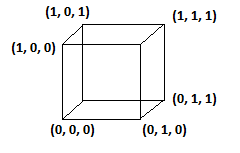
\includegraphics{k23.png}

И еще раз ($K_2 \square K_2 \square K_2 \square K_2$):

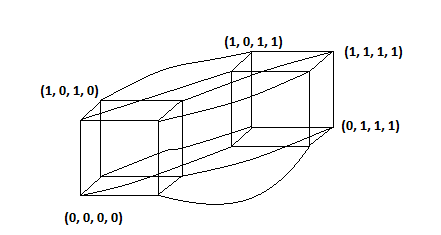
\includegraphics{k24.png}

Тут так и напрашиваются геометрические ассоциации, и это в общем-то неспроста. Действительно, на рисунках по сути изображены отрезок, квадрат, куб и, как мы позже выясним, четырехмерный куб (в свою очередь так же выяснится, что квадрат — это двумерный куб, а отрезок — одномерный куб). По сути каждый раз умножая наш граф на $K_2$, мы вводим еще одно измерение, в котором мы копируем наш куб, и эти два куба склеиваем по вершинам. Четырехмерный куб (то есть его граф), приведенный выше, можно нарисовать в четырехмерном пространстве без пересечения ребер графа. Вообразить себе такое пространство и такой куб оказывается довольно сложно, но представление в виде графов дает об этих кубах (и вообще многомерных объектах) довольно много информации. Например, из рисунка выше мы видим сколько всего у четырехмерного куба будет вершин и ребер, какие вершины какими ребрами соединены, сколько из каждой вершины исходит ребер и так далее. Это согласитесь уже не мало.

Развивая идею можно заметить, что декартово произведение графов ассоциативно и с точностью до переименования вершин коммутативно (и вообще тут можно построить целую арифметику графов при желании, так же как мы поступали с логическими операциями и операциями на множествах). Отсюда в силу ассоциативности сразу следует, что декартово произведение многомерных кубов — тоже является многомерным кубом, и можно сразу понять размерность такого куба.

Топологические приложения изложенного материала идут еще дальше. Есть довольно общий приём триангуляции — разукрашивание поверхностей прилегающими друг к другу треугольниками. Каждая триангуляция является графом. Поверхности называются гомеофорфными, если, представляя, будто они сделаны из резины, можно одну поверхность как-то продеформировать (растянуть-перекрутить без разрывов и склеиваний) в другую поверхность. Это довольно близко к понятию гомеоморфности графов. Позже мы докажем в нашем курсе, что если две поверхности возможно триангулировать гомеоморфными графами, то эти две поверхности сами гомеофорфны, а конструкции, подобные декартову произведению, позволяют выяснить это сравнительно простым путем. Более того, гомеоморфность — это отношение эквиваленции, и таким образом все поверхности распадаются на классы топологически-эквивалентных поверхностей. Дальше на эти классы эквивалентности можно завязать всяческую алгебру и углубляться дальше в абстрактные конструкции сколько вздумается.

Эти рассуждения конечно очень абстрактны и не строги, и пока не очень понятно как именно все это описывается и как с этим работать. Я это рассказал только в обзорных целях для того, чтобы показать куда это все вообще может развиваться, поскольку читатели жалуются, что курс слишком теоретический и не практичен.

{\bfseries Упражнение.} Пусть $P$ — незамкнутая цепь. Постройте (и нарисуйте) граф $P\square K_2$ (такой граф называется лестницей).

{\bfseries Упражнение.} Пусть опять $P$ — незамкнутая цепь. Постройте (и нарисуйте) граф $P\square P$ (такой граф называется сетью).

Следующие упражнения можно решать только при наличии каких-то геометрических образов в голове. Я их никак не объяснял, поэтому материала курса пока явно не хватит для решения, однако вы можете их хотя бы попробовать. Если вы ничего не понимаете, то это не страшно (и даже справедливо), смело пропускайте их — далее в курсе это всё будет рассмотрено более подробно и формально, и тогда к ним можно будет вернуться.

{\bfseries Упражнение.} Докажите, что куб, пирамида и сфера гомеоморфны (их можно триангулировать одним и тем же графом; вершины графа не обязательно могут совпадать с геометрическими вершинами трехмерного объекта — важна лишь возможность его нарисовать).

{\bfseries Упражнение.} Докажите, что если $C$ — это цикл, то $C\square P$ — это цилиндр, и что цилиндр гомеоморфен сфере.

{\bfseries Упражнение.} Докажите, что $C\square C$ — это тор (выглядит как бублик) и он не гомеоморфен сфере.

В общем случае, если нам даны графы $A$ и $B$, то их произведение $A\square B$ строится, как теперь должно быть понятно, следующим образом: каждая отдельная вершина графа $B$ заменяется на точную копию графа $A$, а ребра графа $B$ соответственно заменяются на ребра, соединяющие все соответствующие вершины копий графа $A$.

Но вернемся к нашим менеджерам. Какое они имеют отношение ко всей этой многомерной геометрии? А вот какое.

Каждого менеджера можно условно считать графом $K_2$. Одна вершина этого графа символизирует белую шапку на нём, другая черную, а ребро, их соединяющее — тот факт, что для него эти цвета неразличимы (он не видит какая шапка на нем надета). Тогда несколько менеджеров можно интерпретировать как многомерный куб $K_2 \square K_2 \square \ldots \square K_2$, у которого каждая вершина соответствует некоторому набору шапок на менеджерах. В момент, когда на менеджеров надевают шапки, фактически совершается выбор одной вершины куба. Но никакой отдельный менеджер не знает что это за вершина, так как он не знает цвета собственной шапки — он знает лишь то, что он «находится» в одной вершине куба из двух, то есть его знание может быть охарактеризовано ребром куба.

Пусть, например менеджеров трое, и всем надели белые шапки, что мы будем записывать как $(0, 0, 0)$. Первый менеджер не знает какая на нем надета шапка, и для него выбор стоит между $(0, 0, 0)$ и $(1, 0, 0)$. Для второго между $(0, 0, 0)$ и $(0, 1, 0)$. Для третьего $(0, 0, 0)$ и $(0, 0, 1)$. Это и есть ребра, которые исходят из вершины, характеризующей расстановку шапок.

После того, как менеджеры увидели шапки друг друга, им надо принять решение какой цвет назвать и называть ли его вообще. Поведение менеджеров таким образом можно описать ориентированным графом с теми же вершинами, но где каждое ребро либо удалено, либо заменено на дугу (ребро, направленное в одну сторону). Продолжая прошлый пример, если первый менеджер выберет сказать, что у него белая шапка, это будет представлено дугой $(1,0,0)\to (0, 0, 0)$, если предпочтет сказать, что шапка черная, то это будет дуга $(0, 0, 0)\to (1, 0,0)$. Если предпочтет промолчать, то вершины $(0, 0, 0)$ и $(1, 0, 0)$ вообще не будут инцидентны.

Попытаемся понять, как нам надо выбрать этот орграф таким образом, чтобы менеджеры в большинстве случаев справлялись с задачей. Если у нас в некоторую вершину идет хоть одна дуга, то это значит, что если расстановка шапок будет соответствовать этой вершине, то кто-то из менеджеров назовет цвет своей шапки. Если из какой-то вершины исходит какая-то дуга в другую вершину, то это значит, что при расстаноке шапок для этой вершины менеджер, соответствующей этой дуге, ошибется, и все проиграют. Если какая-то вершина не будет инцидентна никакой другой вершине, то это значит, что при соответствующем расположении шапок, все промолчат, и менеджеры снова проиграют.

Наша задача сводится к такому заданию ориентированного графа, чтобы количество проигрышных вершин (таких, из которых исходят дуги), было как можно меньше, и как можно больше вершин, в которые идет хотя бы по одной стрелке, но для которых нет исходящих стрелок. Такую оптимальную стратегию для трех менеджеров можно выразить следующим рисунком:

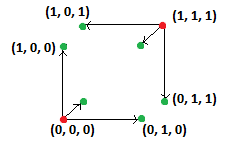
\includegraphics{sol3.png}

Здесь фактически говорится, что если некий менеджер видит, что шапки двух других менеджеров имеют одинаковый цвет, то ему надо назвать цвет противоположный. Это действительно очень простая стратегия: вероятность того, что всем оденут шапку одного цвета меньше, чем вероятность того, что цвета будут все же разными. Поэтому можно предполагать, что существуют все же разноцветные шапки, и поэтому если ты видишь, что у двух менеджеров одинаковые шапки, то на тебе самом с большой степенью вероятности шапка имеет противоположный цвет. До этого решения конечно можно было бы догадаться и без многомерных кубов.

А вот решение для четырех менеджеров:

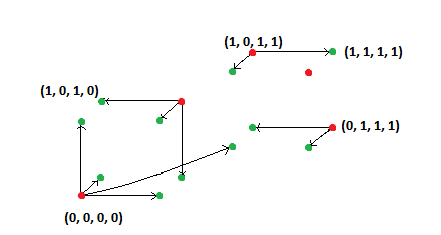
\includegraphics{sol4.png}

Эту стратегию уже так просто не сформулируешь. Если все четверо видят только белые шапки, то надо называть черный цвет. Во всех остальных ситуациях четвертый менеджер вообще молчит, говорят оставшиеся. Если на всех кроме четвертого черные шапки, то все кроме четвертого называют белый цвет. Если на четвертом менеджере черная шапка, то первый менеджер должен молчать. Если второй видит на третьем и четвертом черные шапки, то он должен называть цвет, который видит на первом менеджере. Третий же менеджер должен называть цвет второго менеджера, если он не совпадает с цветом первого. В остальных случаях менеджеры молчат. (Вероятно я где-то ошибся, потому что глядя на этот график можно глаза сломать и я не уверен, что корректно его прочитал; но идея думаю понятна). Решение с трудом можно назвать изящным, но как видно из нашего графа, в большинстве случаев менеджеры все же будут выигрывать. Поэтому это пусть и не красивое (и даже уродливое), но все равно решение. Согласитесь, что если бы это был вопрос жизни и смерти, то оно бы вас устроило.

Если менеджеров больше, то задача решается аналогично, хотя графы будут еще больше по размеру и перебирать придется еще больше вариантов. С этим может справиться компьютер, хотя задача все равно сложная. Какого-то универсального и простого решения к этой задаче видимо не существует, но тем не менее с помощью графов мы смогли получить хоть что-то. Без подобных абстракций и строгой формализвации, задача не решалась бы вообще никак.

Еще хуже была бы ситуация, если бы цветов шапок было бы не два, а больше. Тогда помогло бы следующее понятие:

{\bfseries Определение.} {\slshape Гиперграфом} называется пара $(V, E)$, где $E\subset 2^V$.

Фактически это граф, в котором ребра соединяют сразу множество вершин.

Любой гиперграф может быть представлен с помощью обычного графа. Для этого надо рассмотреть граф, множество вершин которого разбито на два подмножества — одно подмножество вершин соответствует вершинам гиперграфа ($V_0$), а второе ребрам гиперграфа ($V_1$). Множество ребер, инцидентных одной и той же вершине из $V_1$ соответствует грани гиперграфа.

Используя гиперграфы можно решать задачу менеджеров и с произвольным количеством цветов шапок. Задача однако в этом случае становится менее интересной, так как вероятность выигрыша менеджеров резко падает.

Гиперграф — не единственное возможное обобщения понятия граф. Гораздо чаще применяется следующее определение:

{\bfseries Определение.} {\slshape Абстрактным симплициальным комплексом} на множестве $S$ называется множество $\Delta\subset 2^S$, такое, что если $x\in \Delta$, то для любого $y\subset x$ так же $y\in\Delta$. Элементы множества $\Delta$ называются {\slshape абстрактными симплексами}.

Абстрактные симплициальные комплексы удобно строить последовательно: вначале выбирается множество вершин $S$ (так называемые нульмерные симплексы). Затем выбираются обычные ребра графа, соединяющие вершины из $S$ (одномерные симплексы). Затем из различных объединений этих ребер и вершин выбираются трехмерные симплексы, которые можно рассматривать как сплошные пленки, которыми заклеиваются ребра графа. Объединяя эти пленки можно выбрать трехмерные симплексы, затем четырехмерные и так далее. Здесь правда надо следить за тем, чтобы «наклеивая пленки» мы не нарушали условий определения комплекса. Например, если есть грани $\{a, b\}$ и $\{b, c\}$, но нет грани $\{a, c\}$, то наклеить пленку $\{a, b, c\}$ мы не имеем права, поскольку по определению для ее наклеивания требуется так же наличие грани $\{a, c\}$, что неплохо соответствует геометрической интуиции.

Такие конструкции используются опять же в многомерной топологии и с помощью них можно выяснять подробности устройства многомерных объектов. В этом курсе все это будет значительно позже, пока что я привел эти определения лишь для того, чтобы показать каким образом самые базовые понятия теории множеств могут быть полезны простому человеку и как она позволяет простым способом обобщать привычные в общем-то понятия. Написанное в этом параграфе можно смело забыть до поры, это все у нас будет значительно позже.

\section{Функции}

{\bfseries Определение.} {\slshape Функцией}, или {\slshape отображением}, из множества $A$ во множество $B$ (обозначение $f:A\to B$) называется множество упорядоченных пар $f\subset A\times B$, таких что для любого $a\in A$ найдется единственный $b\in B$, такой что $(a, b) \in f$.

Если $(a, b) \in f$, то это часто записывается как $f(a) = b$ или как $f:a \mapsto b$. Множество всех функций $\{f: A\to B\}$ обозначается как $B^A$.

{\bfseries Определение.} Если $f:A \to B$, то множество $A$ называется {\slshape областью определения} функции $f$ и обозначается как $\mathrm{Dom} f$.

Область определения может представлять собой декартово произведение нескольких множеств. В этом случае говорят, что функция является {\slshape функцией нескольких переменных}, где каждое множество соответствует отдельной переменной.

{\bfseries Определение.} Если $f:A \to B$, то множество $B$ называется {\slshape областью значений} функции $f$ и обозначается как $\mathrm{Codom} f$.

{\bfseries Пример.} Логические операции И, ИЛИ, Исключающее ИЛИ, импликация и эквиваленция рассматриваемые нами ранее, являются фунциями $f:B\times B \to B$ (это всё функции нескольких переменных), где $B = \{0, 1\}$. Функция НЕ является функцией типа $f: B \to B$.

{\bfseries Пример.} Объединение и пересечение множеств являются функциями типа $f: S \times S \to S$, где $S$ — некоторое множество, состоящее из других множеств.

{\bfseries Пример.} Любой предикат $F$, заданный на некотором множестве $S$ является функцией типа $F: S \to B$, где $B = \{0, 1\}$.

Если говорить о чистой интуиции, то понятие функции имеет две основных трактовки. Первая — это некоторый объект, который по заданному элементу множества $A$ каким-то образом выдает какой-то элемент множества $B$. Иногда он берет его из таблицы, иногда есть какая-то формула, по которой можно этот самый $b$ вычислить, иногда какая-то написанная на компьютере программа, которая по $a$ дает $b$. Если у нас есть некоторое физическое устройство (например, черный ящик) с клавиатурой, свалившееся из космоса, которое при наборе какого-то числа дает в ответ другое число, и мы не знаем как именно оно это делает — это все равно тоже функция.

Мы можем привести множество примеров функций в быту. Если $A$ — множество женатых мужчин, а $B$ — замужних женщин, то функция, сопоставляющая каждому мужчине в соответствие его жену, является функцией вида $f: A\to B$. Если у нас например есть база данных, в которую мы можем вводить имена мужчин, а она отдает нам в ответ имена их жен, то эта база данных как раз и будет реализовывать данную функцию.

Можно рассмотреть множество рабочих дней, прошедших от начала торгов на Нью-Йоркской фондовой бирже, и каждому дню сопоставить лидеров роста и падения. Если дни обозначить за $D$, а компании за $C$, то такое сопоставление будет функцией вида $D\to C\times C$.

В дальнейшем мы будем временами приводить примеры из кодирования и криптографии. Шифрование и кодирование — это тоже функции. Если $T$ — множество всех возможных текстов, а $B^\infty$ — множество последовательностей нулей и единиц (как это принято в компьютере на низком уровне), кодирование — это функция $f:T\to B^\infty$. Задачей теории кодирования является построение такой функции $f$, чтобы она обладала какими-то полезными свойствами, например чтобы запись была максимально краткой, либо чтобы она была устойчива к ошибкам, и в случае каких-то сбоев можно было восстановить весь текст и по фрагменту кодировки.

Если $K$ — множество ключей, а $C$ — множество шифровок, то шифрование сводится к реализации функции шифрования $E: T\times K \to C$ и дешифрования $D: C\times K \to T$, которые должны быть выбраны таким образом, чтобы не зная ключа $k\in K$ нельзя было восстановить исходный текст $t \in T$ по шифру $c \in C$.

Если $A$ — множество карточных мастей, а $B$ — множество достоинств карт, то функция, которая ставит каждой карте в соответствие ее достоинство, имеет вид $f: A\times B \to B$ и может быть записана формулой как $f: (a, b) \mapsto b$.

Второй интуитивный смысл, который часто имеют функции — это установление соответствия между различными объектами, которое говорит нам что-либо о свойствах этих объектов. Пусть, например, множество $A$ состоит из упорядоченных элементов $a<b<c$, а множество $B$ из элементов $a<b<c<d<e$. Тогда функция $f:A \to B$, которая сопоставляет любому элементу тот же самый элемент другого множества ($f: x\mapsto x$) может показать нам, что множество $A$ в некотором смысле является начальным отрезком множества $B$ — любой элемент последнего множества, не нашедшего себе пары во множестве $A$, будет больше любого другого элемента. Это примитивный пример, но вероятно он как-то продемострирует общую идею (если нет, то позже вероятно вы это поймете на практике).

Рассмотрим более содержательный пример. В первом параграфе мы говорили, что любому предикату на множестве $S$ соответствует подмножество $S$ и наоборот. Это соответствие — тоже функция. Каждый такой предикат — это функция вида $f:S\to B$, и стало быть $f\in B^S$. Тогда функция $p$, которая по предикату дает подмножество, ему соответствующее, имеет тип $p:B^S \to 2^S$. Забегая вперед можно сказать, что $2=\{0, 1\}$ (это будет объяснено в третьей главе), и именно отсюда происходит обозначение для булеана.

Отметим так же, что функции используются часто не только для отображения отдельных элементов, но и для отображения подмножеств элементов.

{\bfseries Пример.} Пусть опять $A$ — множество женатых мужчин, $B$ — замужних женщин, а $f: A\to B$ ставит каждому мужчине в соответствие его жену. Пусть теперь $M\subset A$ — подмножество мужчин, работающих в Макдональдсе. Тогда $f(M)$ — это множество женщин, чьи мужья работают в МакДональдсе.

Это можно формализовать при желании и назвать отдельными словами:

{\bfseries Определение.} Если $f(a) = b$, то $b$ называется {\slshape образом} элемента $a$ по отображению $f$.

{\bfseries Определение.} Множество $f(S) = \{y\in \mathrm{Codom}f|\exists x \in S, f(x) = y \}$ называется {\slshape образом} множества $S$ по отображению $f$.

{\bfseries Определение.} Множество $f^{-1}(y) = \{x | f(x) = y \}$ называется {\slshape прообразом} элемента $y$.

{\bfseries Определение.} Множество $f^{-1}(S) = \{x | f(x) \in S \}$ называется {\slshape прообразом} множества $S$.

Обратите внимание на то, что образом любого элемента является только один элемент, а прообразом является целое множество элементов (вполне возможно, что пустое).

{\bfseries Пример.} Пусть $A = \{a, b, c\}$, $f = \{(a, a), (b, c), (c, c)\}$. Тогда $f^{-1}(a) = \{a\}$, $f^{-1}(b) = \emptyset$, $f^{-1}(c) = \{b, c\}$.

{\bfseries Определение.} Множество $\mathrm{Im} f = f(\mathrm{Dom} f)$ называется {\slshape образом} функции $f$.

Обратите внимание на то, что в общем случае $\mathrm{Im} f \not= \mathrm{Codom} f$. Так, в последнем примере $\mathrm{Im} f = \{a, c\}$, но $\mathrm{Codom}f = \{a, b, c\}$.

{\bfseries Определение.} Единичной функцией на множестве $A$ называется функция $1_A: A\to A$, ставящая любому элементу в соответствие его же самого: $1_A: a\mapsto a$.

{\bfseries Определение.} {\slshape Композицией} функций $f:B\to C$ и $g:A\to B$ называется функция $f\circ g: A\to C$, такая что если $f(b) = c$ и $g(a) = b$, то $(f\circ g)(a) = c$.

{\bfseries Теорема.} Для любой функции $f: A\to B$, $1_B \circ f = f \circ 1_A = f$.

Докзательство в качестве простого упражнения.

{\bfseries Теорема.} Композиция функций ассоциативна: $f\circ (g \circ h) = (f\circ g)\circ h$.

{\bfseries Доказательство.} Достаточно выписать напрямую два значения функции для произвольного элемента $x$, чтобы увидеть это:

Слева: $(f\circ (g \circ h)) (x) = f((g\circ h)(x)) = f(g(h(x)))$

Справа: $((f\circ g) \circ h) (x) = (f\circ g)(h(x)) = f(g(h(x)))$

Как видно, в обоих случаях получается одно и то же значение. \qed

{\bfseries Определение.} Функция называется {\slshape инъективной}, или {\slshape инъекцией}, если $f(a)\not= f(b)$ для любых $a\not= b$.

{\bfseries Определение.} Пусть $f:A\to B$. Функция $f^{-1}_l$, такая что $f^{-1}_l\circ f = 1_A$ называется {\slshape левой обратной}.

{\bfseries Теорема.} Функция имеет левую обратную функцию тогда и только тогда, когда она инъективна.

Докажите эту теорему в качестве упражнения.

{\bfseries Пример.} Любая функция кодирования обязана быть инъективной, поскольку в противном случае была бы возможна ситуация $f(a) = f(b) = c$, и было бы не понятно как мы должны раскодировать $c$ обратно.

{\bfseries Определение.} Если $\mathrm{Im}f = \mathrm{Codom}f$, то функция называется {\slshape сюръективной}, или {\slshape сюръекцией.}

{\bfseries Определение.} Пусть $f: A\to B$. Функция $f^{-1}_r$. такая что $f\circ f^{-1}_r = 1_B$ называется {\slshape правой обратной}.

{\bfseries Теорема.} Функция имеет правую обратную функцию тогда и только тогда, тогда она сюръективна.

Доказательство опять же не сложно и я осталвяю его читателю в качестве упражнения.

{\bfseries Упражнение.} Пусть $f:A \times B \to A$ и $f: (a, b)\mapsto a$. Докажите, что эта функция сюръективна.

{\bfseries Определение.} Если функция одновременно и сюръективна и инъективна, то она называется {\slshape биективной}, либо {\slshape биекцией}.

{\bfseries Теорема.} Если $f: A\to B$ — биекция, то левая обратная функция будет совпадать с правой обратной функцией.

Доказательство снова в качестве не сложного упражнения. Понятно, что в случае с биекциями разница между левой обратной и правой обратной функцией пропадает (в случае же сюръекции или инъекции существует лишь одна из них), и поэтому такая функция называется просто {\slshape обратной}.

Так же полезно заметить, что произвольную инъективную функцию возможно сделать биективной, если заменить ее область значений лишь ее образом, то есть если $C = \mathrm{Im} f$, то вместо функции $f: A\to B$ рассмотреть функцию $f: A \to C$. Легко проверить, что в этом случае функция действительно станет биекцией.

Для сюръекции подобное утверждение тоже верно, но только при отдельных оговорках.

{\bfseries Определение.} Ограничением функции $f: A\to B$ на $S\subset A$ называется функция $f|_S: S\to B$, такая что для любого $x\in S$ верно, что $f|_S(x) = f(x)$.

Несколько более формально и точно, но менее понятно можно написать, что $f|_S = f \cap S \times B$.

Для произвольной сюръективной функции можно было бы попробовать искать такое ограничение этой функции, чтобы она стала биекцией. Предположение это на первый взгляд довольно очевидно, однако оказывается, что оно эквивалентно так называемой аксиоме выбора, которую во-первых нельзя взять и доказать, а во-вторых из которой следует множество парадоксов. Подробнее мы будем обсуждать эту тему далее в этом курсе (и совсем немного в следующем параграфе), пока что можно просто принять к сведению (хотя это и не принципиальной важности факт), что доказать существование такого ограничение невозможно.

{\bfseries Определение.} Множества $A$ и $B$ называются {\slshape равномощными} (обозначение $|A| = |B|$), если существует биекция $f: A\to B$.

Равномощность говорит о том, что элементы множеств $A$ и $B$ можно поставить во взаимооднозначное соответствие. Часто это интерпретируется как то, что они содержат одинаковое число элементов. Это правда довольно опасная интерпретация, что станет ясно, когда мы начнем говорить о бесконечных множествах. Пока же в принципе довольно удобно воспринимать равноможность именно так. имея  правда ввиду, что это сгодится лишь только для довольно маленьких множеств.

{\bfseries Пример.} Пусть $A = \{1, 2, 3\}$, $B = \{a, b, c\}$. Тогда эти множества равномощны, поскольку существует биекция $f=\{(1, a), (2, b) , (3, c)\}$.

{\bfseries Пример.} Пусть $A$ — множество женатых мужчин, а $B$ — множество замужних женщин. Эти множества равномощны.

{\bfseries Упражнение.} Приведите пример неравномощных множеств и двух отображений на них: сюръективного и инъективного.

\section{Формализм}

Как обычно в завершение главы немного пожестим и рассмотрим довольно сложные темы, которые не обязательны для понимания дальнейшего материала, и которые при возникающих сложностях можно пропустить. Если вы молодая, одинокая, красивая девушка из Москвы или около, и вы вдруг поймете что здесь написано, то вам надо обязательно написать мне письмо на почту. Я на вас женюсь.

Обычно рассмотрение формализма теории множеств начинают с обсуждения парадокса Рассела, на примере которого объясняются ряд тонкостей аксиом теории множеств и мотивируются определения. Мы не будем исключением.

{\bfseries Парадокс Рассела.} Пусть $U$ — множество всех множеств. $A = \{x\in U|x\not\in x\}$, то есть множество таких множеств, которые не содержат себя самого в качестве элемента. Вопрос: принадлежит ли $A$ самому себе, то есть верно ли, что $A\in A$?

Если предположить, что $A\in A$, то по определению $A$, он не должен быть элементом $A$. Если $A\not\in A$, то по определению $A$, $A \in A$. Это сильно напоминает парадокс брадобрея, рассмотренный в первой главе, и утверждение парадокса Рассела на самом деле легко сводится к тому же самому утверждению: $\exists A\forall x\in A (x\in A \leftrightarrow x\not\in x)$. Однако в качестве $x$ мы можем взять $A$ и получить запись $A\in A \leftrightarrow A\not\in A$. Это высказывание всегда ложно.

Когда мы рассматривали парадокс брадобрея, то придя к такому выражению мы сделали вывод о том, что изначальная постановка задачи была некорректна — такого брадобрея просто не могло существовать. Так и здесь очевидно, что множества $A$, описанного в условии парадокса, очевидно не может существовать. Стало быть где-то мы использовали запись, которую мы использовать не имеем права. Первое предположение, которое обычно делают люди, глядя на этот парадокс, что некорректна запись $x\in x$, и соответственно первое желание — запретить множеству быть элементом самого себя.

Аксиоматика Цермело-Френкеля (сокращенно ZF), которую мы будем рассматривать в этом параграфе, как раз запрещает выражения вида $x\in x$. Для такого запрета специально вводится аксиома Foundation Axiom: «Для любого непустого множества $x$ найдется такое $y\in x$, что $x$ и $y$ не пересекаются». Такая сложная формулировка на самом деле оправдана. Если бы вместо нее мы написали что-то простое вроде $\neg \exists x, x\in x$, то в таком виде эта аксиома все равно продолжала бы приводить к парадоксам вроде парадокса Рассела. Например, оказалась бы корректной запись $x=\{y\}$, $y=\{x\}$. В этом случае, действительно, $x\not\in x$, но однако $x\in y\in x$, а это ничуть не лучше того, что было изначально.

При этом важно заметить, что даже при этой аксиоме, у нас возможна ситуация, когда некоторый элемент множества является одновременно и его подмножеством: $x\in y \wedge x\subset y$. Например, вот: $a = \{b, c\}$, где $c=\{ b\}$. Очевидно, что $c\in a \wedge c\subset a$.

Может показаться, что эта ситуация тоже нежелательна. Однако, это не так. На самом деле вся арифметика построена именно на таких множествах. Если быть точным, то в современной математике натуральные числа определены следующим образом:

0) $0 = \emptyset$

1) $1 = 0 \cup \{0\} = \{0\}$

2) $2 = 1 \cup \{1\} = \{0, 1\}$

3) $3 = 2\cup \{2\} = \{0, 1, 2\}$

4) $4 = 3 \cup \{3\} = \{0, 1, 2, 3\}$

И так далее. В общем случае определена операция инкремента $S: n\mapsto n\cup \{n\}$, через которую и определяется множество натуральных чисел, обозначаемое символом $\mathbb{N}$. Сама функция инкремента часто обозначается как $+1$, то есть $S(n) = n+1$. $+1$ в данном случае не какая-то операция над числом и единицей, а просто другое обозначение для функции $S$. Мы пока примем сформулированное определение натуральных чисел как факт, а подробнее будем рассматривать его в следующей главе.

Как видно, накладывая ограничения на структуру множеств, Foundation Axiom тем не менее оставляет значительный простор для конструирования множеств, и это еще одна причина, по которой она формулируется именно в таком виде.  Иные виды формулировок, которые могли бы придти на ум, могли бы не оставить нам возможности определить подобным образом натуральные числа. Мы конечно могли бы определить их и как-нибудь по-другому, однако приведенное определение пока является наиболее простым и удобным из всех известных науке. Об этом опять же будет в следующей главе.

Тем не менее с этой аксиомой оказывается все не совсем гладко, о чем свидетельствует следующая теорема.

{\bfseries Теорема.} В предположении Foundation Axiom, не существует бесконечной последовательности $x_1, x_2, x_3, \ldots$ такой, что $x_2 \in x_1$, $x_3 \in x_2$, $x_3 \in x_4, \ldots$, то есть последовательности, в которой каждый элемент является множеством, причем каждый элемент является так же элементом предыдущего элемента.

Прежде чем перейти к доказательству, сделаем некоторые замечания по терминологии.

{\bfseries Определение.} {\slshape Последовательностью} элементов множества $A$ называется функция $x:\mathbb{N}\to A$. Элементы $x(n)\in A$ называются {\slshape элементами последовательности} и обозначаются как $x_n$.

При перечислении элементов последовательности, обычно предполагают, что первым элементом является $x_1$, затем $x_2$ и так далее. Формально это не совсем соответствует определению, которое мы только что привели: элементы последовательности мы начинаем нумеровать с единицы, однако множество натуральных чисел «начинается» с нуля. Чтобы добиться точности, мы могли бы либо нумеровать элементы последовательности начиная нулем, либо определять последовательность как отображение $\mathbb\{N\}\setminus \{0\} \to X$. На практике же эта неточность ни на что не влияет и поэтому можно оставить все как есть.

Если в нашем условии теоремы рассмотреть некоторое множество множеств $U$ и вспомнить о функции инкремента $+1$, то теорему можно переформулировать таким образом:

{\bfseries Теорема.} В предположении Foundation Axiom, не существует последовательности $\{x_n\}$ такой, что $x_{n+1} \in x_n$.

{\bfseries Доказательство.} Предположим противное. Пусть $f: \mathbb{N}\to U$ — такая функция, что $f(n+1) \in f(n)$. Foundation Axiom требует, чтобы существовало $A\in \mathrm{Im} f$, такое, что $A \cap \mathrm{Im}f = \emptyset$. Однако для любого $A\in \mathrm{Im} f$ найдется такое $n$, что $A = f(n)$ в силу определения $f$. Отсюда $f(n+1) \in A$ и $f(n+1)\in \mathrm{Im}f$. Это значит, что $f(n+1)\in A \cap \mathrm{Im}f$, то есть $A$ и $\mathrm{Im}f$ все же пересекаются вопреки нашему предположению. Полученное противоречие доказывает теорему. \qed

Рассмотрим множество людей не Земле. Каждый из людей состоит из множества органов. Каждый орган из множества тканей. Ткани — из клеток. Клетки из органоидов, органоиды из молекул, молекулы из атомов и так далее. Это не очень точная и не очень формальная последовательность с научной точки зрения, но для наших целей этого вполне достаточно. Атом можно продолжать разбивать на субатомные частицы, их можно разбивать далее, получив кварки, которые, пока только предположительно, могут состоять из преонов (это открытый вопрос науки). Если будет доказано существование преонов, вполне вероятно, что встанет вопрос о том, из чего состоят преоны. В общем виде можно задаться таким вопросом, сформулированную еще в древние времена: можно ли различные объекты физического мира разбивать на составные части сколь угодно долго, либо же мы неминуемо придем к некоторым неделимым составным частям?

Foundation Axiom внезапно отвечает на этот вопрос: да, мы обязательно должны придти к неделимым составным частям. Foundation Axiom конечно работает с формальными множествами, а приведенные физические рассуждения с объектами реального физического мира, поэтому считать, что Foundation Axiom действительно говорит что-то о реальном мире, мы не можем. Однако же подобная интерпретация наводит на мысли о том, что данная аксиома вероятно и не особо-то хороша.

Как мы говорили, аксиоматика ZF, которую мы сейчас рассмотрим, все же содержит в себе Foundation Axiom, однако, ZF не единственная возможная формализация теории множеств. Существуют и другие системы аксиом, в которых, наоборот, используется Anti-Foundation Axiom (кратко AFA, которая тоже может формулироваться по-разному). Простейший вариант такой аксиоматики это так называемая New Foundation Set Theory, в которой на уровне аксиом определяются ориентированные графы, допускающие циклы (дуги вида $(a, a)$), и AFA явно постулирует, что каждая вершина графа является множеством.

«Как же тогда в New Foundation обстоит дело с парадоксом Рассела?» — спросит читатель, если он еще тут. Ответ на этот вопрос неожиданный: на самом деле парадокс Рассела вообще почти никак с Foundation Axiom не связан. Сама постановка парадокса содержит множество других внутренних противоречий, которые и приводят к нему, но эти противоречия разрешаются и без Foundation Axiom. Проблема с записью $x\in x$, которую мы пытались разрешить выше, оказывается, является лишь «наведенным эффектом» от других проблем формулировки, а Foundation Axiom при всей своей очевидности, оказывается, что не особо-то и нужна.

Прежде чем перейти к формулировке аксиом ZF, мы должны внести ясность с понятиями логики из первой главы. В первом главе при определении понятий логики, мы активно пользовались теорией множеств. Даже само понятие теории мы формулировали как множество формул. После, определяя понятия теории множеств, мы пользовались логикой. Сейчас нам предстоит переформулировать все что было сказано заново, но только избавившись от порочных кругов.

Итак, нам надо с чего-то начать. Увы, чтобы определить какое-то понятие, нам неминуемо необходимо пользоваться другими понятиями, которые тоже в свою очередь надо как-то определять. Поскольку бесконечную цепочку определений мы физически не можем построить, нам придется смириться с тем, что у нас будет одно базовое понятие, которое не будет иметь никакого определения. Таким понятием для нас станет понятие {\slshape символа}.

Говоря неформально, символ — это некоторая закорючка, которую мы можем нарисовать на листе бумаги. Мы будем считать, что различных символов очень много (сколько угодно сколько потребуется) и мы можем отличать один символ от другого. Определять более строго мы это понятие не будем и примем понятие символа за основу, на которой мы будем строить нашу теорию.

Следующие символы будем называть {\slshape логическими символами}:

— {\slshape логические связки} $\neg$, $\wedge$, $\vee$, $\rightarrow$ и $\leftrightarrow$;

— {\slshape квантификаторы} $\forall$, $\exists$;

— {\slshape равенство} $=$;

— {\slshape переменные}, просто некоторый набор до сих пор не задействованных символов.

Так же будем выделять {\slshape нелогические символы} (это так же просто классификация неиспользуемых ранее символов):

— символы {\slshape отношений}{\slshape };

— символы {\slshape операций};

— {\slshape константные} символы.

Это все пока просто классификация. Скажем, аксиоматика ZF требует лишь одного символа отношения $\in$. Можно было бы рассмотреть дополнительно символы вроде $\cup$, $\cap$, $\bigtriangleup$ и подобных в качестве операций, а символ $\emptyset$ в качестве константного символа, однако аксиомы ZF не используют их, как будет видно ниже. Я повторюсь, что на данный момент мы не наделяем символы никаким смыслом — для нас это пока не более чем закорючки на бумаге, которые мы пока просто классифицировали без какой-либо особой логики.

{\bfseries Определение.} {\slshape Термом} называется либо константный символ, либо переменная, либо запись $f(a, b, \ldots, z)$, где $a, b, \ldots, z$ — некоторые прочие термы, а $f$ — символ операции.

{\bfseries Определение.} {\slshape Атомом} называется либо запись $a = b$, где $a$ и $b$ — термы, либо запись $f(a, b, \ldots, z)$, где $a, b, \ldots, z$ — некоторые прочие термы, а $f$ — символ отношения.

{\bfseries Определение.} {\slshape Формулой} называется одна из следующих записей:

— отдельный атом является формулой;

— если $\phi$ и $\psi$ являются формулами, то записи вида $\neg \phi$, $\phi \wedge \psi$, $\phi \vee \psi$, $\phi \rightarrow \psi$, $\phi \leftrightarrow \psi$ так же являются формулами;

— если $\phi$ — формула, а $v$ — переменная, то $\forall v \phi$ и $\exists v \psi$ так же являются формулами

{\bfseries Определение.} Переменная $v$ в составе формулы называется {\slshape свободной}, если перед этой формулой не написано $\exists v$ или $\forall v$

{\bfseries Определение.} {\slshape Предложением} называется формула без свободных переменных.

Приведенные нами определения несколько упрощены, но в целом достаточны. Например, с точки зрения определений, данных выше, запись $a\cap b$ не является формулой, однако формулой является $\cap(a, b)$. Мы могли бы расширить наши определения, чтобы покрыть более широкий класс формул, но это был бы довольно скучный бессодержательный рассказ в угоду формализму. При желании формально это может проделать читатель самостоятельно, это не сложно. Мы же двинемся дальше, а для краткости будем полагать, что записи вроде $a\cap b$ являются сокращением записей в соответствии с определениями. Для нас важнее сейчас понять общую идею, а не достичь максимальной корректности с формальной точки зрения.

Теперь можно вспомнить правила вывода из первой главы. Они формулировались просто как правила, по которым можно преобразовывать формулы (хотя само понятие формулы мы строго не определяли). Например, правило modus ponens говорило, что две формулы $\phi$ и $\phi\rightarrow\psi$ можно преобразовать в формулу $\psi$. Эти правила можно применять к произвольным формулам, не наделенных никаким смыслом. Это как раз наш случай. Мы будем их применять просто к закорючкам на бумаге, совершенно не думая о том, что эти закорючки что-то вообще значат.

В общем виде теперь построение теорий будет выглядеть так: из некоторого начального набора предложений, называемых аксиомами, по правилам вывода, мы будем получать некие другие предложения, называемые теоремами. В самом общем виде смысла в этом — ноль. Однако если в качестве аксиом взять какие-то предложения, которые мы можем осознанно интерпретировать как какие-то имеющие физический смысл, то наши выводы теорем уже оказываются полезными.

То есть если подумать, то все человеческие рассуждения — это на самом деле некоторое преобразование высказывания языка. Любые природные или логические явления мы записываем на бумаге, и как бы мы не старались, они все равно в результате описываются словами, смысл которых ровно тот, которым мы их наделяем. Из каких-то предложений человеческого языка мы по некоторым правилам вывода можем строить некоторые рассуждения. Сейчас мы делаем то же самое, но только более формально: мы строго определили само понятие предложения и набор правил, по которым мы можем строить рассуждения. При кажущейся абстрактности и оторванности от физического мира, это на самом деле единственное что нам доступно и это именно то, как строятся все умозаключения и рассуждения.

Доказательства первой главы были конечно не строгими и неформальными, в свете того, что я говорю сейчас. Увы, провести многие из них более формально и не получится вовсе. Весь материал первой главы был нацелен лишь на то, чтобы дать неформальную интуицию, касающуюся того, почему вообще мы можем наделять наши формулы интерпретацией, и почему отдельные правила вывода логично было бы принять как верные. Строго доказать этого конечно нельзя.

Впрочем, первый параграф был довольно большой, и даже в том виде как мы сформулировали понятие теории, набор теорем логики, которые мы предположительно можем использовать, тоже объемный, и все это предлагается принять на веру, основываясь на каких-то неформальных рассуждениях. Чтобы объем принимаемого на веру оказался меньше, можно в принципе договориться о том, что многие логические символы являются лишь сокращениями для длинных записей. Так, можно считать, что $x\vee y$ — это не более чем сокращенная форма записи для $\neg (\neg x \wedge \neg y)$, а $\exists x P(x)$ — сокращенная форма записи для $\neg \forall x \neg P(x)$. Правила вывода так же многие можно в этом случае либо выкинуть, либо доказать используя только преобразования формул.

Прежде чем окончательно сформулировать аксиомы Цермело-Френкеля, сделаем еще одну ремарку. До сих пор мы говорили, что множество — это набор элементов. Что такое элементы мы тем не менее не определяли. Говоря теперь о формальных символах, мы вообще больше никак не можем разграничить понятие множества и его элемента, у нас в соответствии с определением формулы есть лишь нелогические константы и логические переменные. Это может показаться довольно большим недостатком сформулированной нами логической системы, и долгое время при задании аксиом теории множеств математики вводили специальные предикаты, которые для каждой константы определяли является ли она множеством или нет. С учетом того, что любое множество может быть элементом кого-то другого множества, деление проводилось между элементами и урэлементами, которые множествами никак не являлись. Позже однако выяснилось, что деление на элементы и урэлементы излишне — если предположить, что в нашей теории не существует в принципе ничего кроме множеств, то мы ничего в действительности и не потеряем, а лишь наоборот сделаем нашу теорию проще.

Вот теперь мы можем формулировать аксиомы Цермело-Френкела (ZF):

{\bfseries 1. Extensionality Axiom}: $\forall x \forall y (\forall z (z \in x \leftrightarrow z \in y) \rightarrow x = y)$

Эта аксиома утверждает, что множество полностью определяется своими элементами, то есть если множества $x$ и $y$ состоит из одних и тех же элементов, то $x=y$. Довольно разумное требование, здесь сложно как-то еще это прокомментировать.

{\bfseries 2. Foundation Axiom}: $\forall x(\exists y (y\in x)\rightarrow \exists y(y\in x\wedge \neg \exists z (z\in x \wedge z\in y)))$

Возможно после того, как я сформулировал эту аксиому выше словами обычного русского языка, у вас могло бы возникнуть желание записать эту аксиому как-то вроде $\forall x \not= \emptyset \exists y\in x, x\cap y = \emptyset$. Такая запись однако не может являться предложением нашей теории, так как у нас на данный момент пока не определены $\emptyset$ и операция $\cap$. Поэтому приходится расписывать это все подробно. Попробуйте разобраться каким именно образом предложение выше выражает желаемый смысл аксиомы.

Напомню, что реально большого смысла эта аксиома не несёт и используется лишь в узких областях, связанных непосредственно с самой теорией множеств — как мы увидим далее, все более-менее стандартные ветви математики никак не опираются на эту аксиому. Парадок же Рассела разрешается на самом деле с помощью следующей аксиомы:

{\bfseries 3. Comprehension Scheme Axiom}: Для каждой формулы $\phi$ со свободными переменными $v_1, \ldots, v_n, x$ верно, что $\forall z \exists y \forall v_1 \ldots \forall v_n (x\in y \leftrightarrow x \in z \wedge \phi(x, v_1, \ldots, v_n))$.

Опять же выглядит страшно, но это станет понятнее, когда мы изложим ее смысл. Изначальный посыл этой аксиомы дать возможность формулировать множества по заданной формуле. Мы говорили уже о о том, что каждый предикат дает возможность формировать подмножество, и смысл этой аксиомы в том, что нам нужна возможность формировать множества типа $\{x|\phi(x)\}$.

При заданном фиксированном $\phi$ можно было бы сформулировать эту аксиому как-то так: $\exists y \forall x (x\in y \leftrightarrow \phi(x))$. Однако, эта формулировка привела бы все к тому же парадоксу Рассела, если определить $\phi(x) = x \not \in x$. Действительно, в этом случае $\exists y \forall x (x\in y \leftrightarrow x\not \in x)$, и если положить $x=y$ (мы имеем на это право из-за квантора общности), то получим противоречие $y \in y \leftrightarrow y\not \in y$.

Чтобы избежать парадокса Рассела в данном случае, мы должны потребовать, чтобы можно было формировать не произвольные множества, а лишь подмножества некоторых уже существующих множеств: $\forall z \exists y \forall x (x\in y \leftrightarrow x \in z \wedge \phi(x))$. Данная формальная уловка действительно «лечит» парадокс Рассела: теперь для формулы $x \in y \leftrightarrow x \in z \wedge x\not \in x$ всегда можно взять в качестве $y$ пустое множество, и оба атома $x \in y$ и $x \in z$ окажутся в этом случае ложны, что сделает истинной эквиваленцию (вспоминаем первую главу).

Здесь есть два тонких места. Первое заключается в том, что мы пока не определили понятие пустого множества. Однако с помощью Comprehension Axiom это делается довольно легко, если сформировать подмножество некоторого множества $z$ по предикату $x \not= x$: $\emptyset = \{x \in z |x \not= x\}$. Понятно, что такое множество не содержит ни одного элемента, это же можно считать и как определение пустого множества (если бы нашелся такой $y$, который принадлежал бы определенному нами множеству, то было бы $y\not= y$, что всегда ложно). В силу Extensionality Axiom такое множество единственно, и мы имеем право ввести следующее определение:

{\bfseries Определение.} $\emptyset$ это уникальное множество, такое что $\forall x (x\not\in \emptyset)$.

Второе тонкое место заключается в потенциальной возможности существования множества всех множеств. Если предположить, что существует такое $z$, что $\forall x (x \in z)$, то в фомуле $y \in y \leftrightarrow y\in z \wedge y \not \in y$, рассматриваемой выше, даже если $y = \emptyset$ использованный нами для разрешения парадокса, будет верным $y \in z$, и тогда выражение $y \in y \leftrightarrow y\in z \wedge y \not \in y$ окажется ложным. Отсюда следует следующая теорема:

{\bfseries Теорема.} $\neg \exists x \forall y (y \in x)$.

Это и есть теорема о том, что не существует множества всех множеств. Предположение же парадокса Рассела «Пусть $U$ — множество всех множеств» уже само по себе заключает в себе противорение.

Как теперь видно, парадокс Рассела кроется совершенно не в Foundation Axiom, а в Comprehension Axiom, хотя на первый взгляд казалось очевидным совершенно другое. Реальная причина парадокса не в возможности написать формально $x\in x$ (от такой возможности мы в действительно не можем уйти, если пользоваться определениями формул и теорий как мы их определили), а в слишком вольных терминах при определении подмножеств и самом предположении о существовании множества всех множеств.

Но вернемся к аксиоме. Общий ее смысл я думаю теперь понятен. Переменные $v_i$ необходимы лишь для обобщения аксиомы на случаи формул с несколькими свободными переменными, не более того (рассмотренные нами выше примеры имели лишь одну свободную переменную). Может возникнуть еще вопрос почему мы саму формулу $\psi$ не снабдили квантором $\forall$, ведь в этом случае мы могли бы записать аксиому без дополнительных слов вроде «для каждой формулы $\psi$...».

Дело в том, что квантор мы имеем право навешивать лишь на переменные, а формула переменной понятное дело не является. Поэтому несмотря на интуитивное желание написать $\forall\psi$, делать мы этого не имеем права. При этом как уже говорилось, любое предложение это некоторая вполне конкретная запись. Предложение не может содержать в себе «некоторую произвольную формулу», потому что в терминах «некоторой произвольной формулы» с формальной точки зрения было бы не понятно как совершать логические выводы и что вообще внутри себя эта формула может иметь.

Поэтому фразу «для каждой формулы $\phi$» надо трактовать как то, что на самом деле для каждой отдельной формулы $\psi$ мы записываем отдельную аксиому Comprehension Scheme с этой вот конкретной формулой. Всего формул у нас бесконечное число, и соответственно аксиом у нас получается бесконечно много. Это, однако, ничему не противоречит, просто это надо иметь ввиду. По этой причине говорят, что $ZF$ — бесконечная система аксиом.

Возможность формировать подмножества с помощью Comprehension Scheme ведет так же в козможности определить операцию пересечения множеств:

{\bfseries Определение. }$\cap z = \{x \in a| \forall y \in z, x\in y\}$ для произвольного $a \in z$.

Здесь $z$ можно интерпретировать как множество множеств, которые пересекаются операцией $\cap$. Пересечение лишь двух множеств (то что мы определяли ранее) определяется отсюда как $A\cap B = \cap\{A, B\}$.

Возникает желание определить аналогичным образом и объединение множеств. Для объединения, однако, оказывается, что сформулированных до сих пор аксиом недостаточно. Comprehension гарантирует лишь существование подмножеств, но однако для произвольных $a$ и $b$ совершенно не факт, что будет существовать множество, содержащее их обоих. Разным аспектам этого посвящается следующие три аксиомы.

{\bfseries 4. Pairing Axiom}: $\forall a \forall b \exists z (a\in a \wedge b \in z)$.

Напрямую однако эта аксиома не говорит о том, что для любых $a$ и $b$ существует множество $\{a, b\}$. Оно действительно существует, но для того, чтобы его получить, необходимо применить Comprehension Scheme. С помощью Pairing Axiom мы можем гарантировать существование некоторого $z$ который будет содержать $a$ и $b$ в том числе возможно наряду и с некоторыми другими элементами. Однако из этого мы все же можем выразить подмножество $\{a, b\} = \{x \in z| x = a \vee x = b\}$.

Если в рассуждениях выше задать $a = b$, то можно утверждать, что для любого $a$ существует так же множество $\{a\}$, что тоже ранее было не очевидно.

Используя возможность строить множества $\{a, b\}$ мы теперь можем определить и упорядоченные пары как $(a, b) = \{a, \{a, b\}\}$. Выглядит возможно странно, но действительно для множества $\{a, \{a, b\}\}$ всегда можно определить его элементы, и более того их порядок. Это именно то что требовалось от упорядоченных пар, и определить их по-другому конечно было бы можно, но мы все равно как-то были бы обязаны действовать исходя из определения множеств.

{\bfseries 5. Union Axiom:} $\forall f \exists z \forall y \forall x (x \in y \wedge y \in f \rightarrow x \in z)$.

Здесь можно интерпретировать $f$ как некоторое множество множеств, обозначаемых в данном случае как $y$, элементы которых в свою очередь обозначаются как $x$. Множество $z$ — это некоторое множество, содержащее в качестве подмножества все $y \in f$, то есть их объединение. По Comprehension Scheme опять же можно получитьи точное объединение множеств:

{\bfseries Определение.} $\cup z = \{x \in a|x\in y, y\in z\}$, где $\forall y (y \subset a)$.

Здесь я для удобства ввел символ $\subset$. Его можно трактовать как сокращенную форму записи для $\forall x (x\in A \rightarrow x \in B)$, что впрочем мы и определяли в первом параграфе (я просто отмечаю на всякий случай, что в данном случае нет нарушения определенного нами формализма и всё легко определяется).

Аналогично с пересечением можно определить и объединение лишь двух множеств $A\cup B = \cup \{A, B\}$.

Рассмотренные до сих пор аксиомы уже гарантируют нам существование натуральных чисел: для любого $n$ можно определить $x\cup\{x\}$, а так же мы уже имеем $\emptyset$. Не хватает только пока определния функций и отношений, определение которых требует наличия декартова произведения. Его возможно ввести с помощью следующей аксиомы.

{\bfseries 6. Replacement Scheme Axiom:} для каждой формулы $\psi$ со сводобными переменными $x, y, v_1, \ldots, v_n$ верно, что $\forall X \forall v_1 \ldots \forall v_n (\forall x\in X \exists ! y \phi(x, y, v_1, \ldots, v_n) \rightarrow \exists Y \forall x \in X \exists y \in Y \phi(x, y, v_1, \ldots, v_n))$.

В этой аксиоме мы использовали сокращение $\exists!y$ для фразы «существует единственный $y$». Запись $\exists!x\phi(x)$ можно рассматривать как сокращенную форму для $\exists x \phi(x) \wedge \neg \exists y (y\not=x \wedge \phi(y))$.

По аналогии с Comprehension Scheme данная аксиома является на самом деле сразу целым набором аксиом, по одной для каждой возможной формулы. Так же по аналогии с Comprehension Scheme переменные $v_1, \ldots, v_n$ служат лишь для обощения аксиомы и не несут особо глубокого смысла.

Мотивация за этой аксиомой такая: пусть $\phi(x, y)$ — описание некоторой функции $X\to Y$. На самом деле понятия функции у нас пока нет, поэтому правильнее говорить, что это не функция, а формула, такая что $\forall x\in X \exists!y \phi(x, y)$. Логично, что образ этой функции $\{y|\exists x \in X \phi(x, y)\}$ должен являться множеством. Из аксиом 1-5 этого доказать не получится, поэтому это выражает отдельная аксиома Replacement Scheme. Так же как и Pairing Axiom она требует лишь существования некоторого надмножества, содержащего множество $Y$, но далее точное множество $Y$ как обычно можно получить применив Comprehension Scheme.

С помощью Replacement Scheme можно определить декартово произведение. Во-первых вспомним, что для любых $a\in A$ и $b\in B$ мы уже успешно определили упорядоченную пару $(a, b)$. Тогда, если зафиксировать некоторое $b$, можно рассмотреть отображение $a \mapsto (a, b)$. На языке формул это можно записать как $\forall a\in A \exists!z (z = (a, b))$. Образом этого отображения должно быть множество $A\times\{b\} = \{(a, b)| a\in A\}$, которое действительно будет являться множеством по Replacement Scheme.

Определив $A\times\{b\}$ мы можем рассмотреть отображение $b\mapsto A \times \{b\}$ (или в виде формулы $\forall b\in B \exists! z (z = A\times\{b\})$) и по аналогии образом этого отображения будет множество $X = \{A\times \{ b \} | b \in B\}$. Декартово произведение теперь можно определить как $A\times B = \cup X$.

Отсюда можно уже определять отношения, функции, да и вообще все что угодно. Таким образом, всё, рассматриваемое до сих пор, мы смогли определить и доказать используя только первые 6 (даже 5 за вычетом Foundation) аксиом. Следующие аксиомы мы сформулируем очень кратко, так как для наших целей они пока не нужны и потребуются значительно позже, и соответствующие комментарии по их поводу у нас будут позже.

{\bfseries 7. Infinity Axiom:} $\exists x (\emptyset \in x \wedge \forall y \in x ((y\cup\{y\}\in x)))$

Эта аксиома гарантирует, что все натуральные числа все же образует множество $\mathbb{N}$. Без нее мы могли бы работать с натуральными числами, но не могли бы работать с множеством натуральных чисел собственно как со множеством. Например, мы не могли бы определить множество $\mathbb{N}\times\mathbb{N}$, без которых затруднительно определить арифметику отрицательных и рациональных чисел (будет позже в этом курсе).

{\bfseries 8. Power Set Axiom.} $\forall x \exists y \forall z (z\subset x \rightarrow z\in y)$

Гарантирует существование множества $2^X$ для любого $X$. Необходима для определения вещественных чисел (опять же будет позже).

Эти восемь аксиом собственно и образуют аксиоматику ZF. К перечисленным аксиомам почти всегда добавляется еще следующая «аксиома выбора», вместе с которой аксиоматика носит название ZFC:

{\bfseries 9. Choice Axiom.} Формулировку разобьем на несколько строк:

$\forall A \forall B \forall f\subset A\times B \\(\forall x \in A \exists! y\in B, (x, y)\in f\rightarrow\\ (\exists S\forall y\in B(\exists x\in A, (x, y)\in f \rightarrow \\ \exists!x\in X, (x, y)\in f\cap S\times B)))$

Выглядит, опять же, страшно, но на деле ничего особого. Все, что здесь сказано — это то что из произвольного множества мы можем выбрать некоторый элемент, и на деле формальная запись этой аксиомы никогда не применяется — обычно просто говорят «возьмём некоторый элемент $x$ из множества $X$», и это как раз подразумевает использование аксиомы выбора. Ниже я кратко опишу как выбор элемента из множества связан с формальной записью выше, но это в принципе уже программа максимум — на практике подобные рассуждения да и само приведенное формальное определение совершенно излишни и никем никогда не рассматриваются.

Итак, пусть нам дана функция $f: A\to B$. Каждый $b \in B$ имеет прообразом некоторое множество. Причем для разных $b\in B$ эти прообразы не пересекаются. Мы можем сказать, что на $A$ задано отношение эквивалентности следующим образом: $x\sim y$, если $f(x) = f(y)$. Тогда выбор некоторого элемента из множества — это все равно что выбор элемента из класса эквивалентности. Пусть мы выбрали из каждого такого класса эквивалентности по одному представителю, и сформировали из них множество $S$. Ограничение $f|_S$ будет инъективным. Возможность такого выбора (то есть утверждение аксиомы выбора) эквивалентно возможности такого ограничения произвольной функции $f$, чтобы она стала инъективной.

Осталось формализовать эти понятия. Если $f: A\to B$, то формально это можно записать как $f\subset A\times B \wedge \forall x \in A \exists!y\in B, (x, y)\in f$

Если дополнительно к этому функция $f$ инъективна, то мы можем сказать, что $\forall y\in B (\exists x\in A, (x, y)\in f \rightarrow \exists!x, (x, y)\in f)$. Здесь необходима проверка $\exists x\in A, (x, y)\in f$, чтобы убедиться в том, что конкретный $y\in B$ вообще имеет прообраз.

Теперь, вспомнив, что $f|_S = f\cap S\times B$, мы после некоторых раздумий получаем формулировку аксиомы выбора в том виде, как я ее привел.

Из аксиомы выбора следует множество парадоксов, самый пожалуй душещипательный их которых следующий:

{\bfseries Парадокс Банаха-Тарского.} Любой шар можно разрезать на конечное число кусков, а потом из этих кусков собрать два таких же точно шара.

Этого парадокса не стоит пугаться — в нем нет никаких противоречий и нет ничего непонятного. Мы это докажем далее в нашем курсе, когда вы будете к этому готовы. Пока что же мы отложим подробное рассмотрение аксиомы выбора до времен, когда мы уже освоимся на практике со следствиями остальных аксиом и поупражняемся в работе с бесконечными множествами.

\section{Теоремы Гёделя}

В прошлом параграфе мы строго определили аксиомы теории множеств. Сейчас мы копнем немного глубже и попытаемся понять насколько приведенный нами формализм полноценен.

Когда мы в первой главе говорили о теориях в самом общем виде, то мы упоминали два возможных свойства теорий: полноту и непротиворечивость. Напомню эти определения (теперь в несколько более формальном виде):

{\bfseries Определение.} Теория $T$ называется {\slshape полной}, если для любого предложения $\phi$ либо $T\vdash\phi$, либо $T\vdash\neg\phi$.

{\bfseries Определение.} Теория $T$ называется {\slshape непротиворечивой}, если ни для какой формулы не может быть одновременно $T\vdash \phi$ и $T\vdash\neg\phi$.

В первой главе мы так же доказывали, что из противоречивых теорий можно вывести любую формулу. Этот факт будет нами использоваться ниже.

Является ли ZFC полной и непротиворечивой? Ответ на этот вопрос дают следующие две теоремы (доказательства мы проведем ниже, а пока только сформулируем и обсудим эти утверждения):

{\bfseries Первая теорема Гёделя о неполноте.} Никакая аксиоматическая система, в которой возможно описать арифметику натуральных чисел, не является полной.

{\bfseries Вторая теорема Гёделя о неполноте.} Ни для какой аксиоматической системы, в которой возможно описать арифметику натуральных чисел, невозможно доказать ее непротиворечивость.

То есть результаты прямо скажем неутешительные. Если говорить простыми словами, то здесь говорится о том, что существуют некоторые теоремы, которые мы никогда не сможем доказать, причем доказуемость этих теорем совершенно никак не зависит от системы аксиом, которую мы придумаем. Что бы мы там ни напридумывали вместо ZFC, все равно полученная аксиоматика будет неполной.

Это, впрочем, не особенно большая проблема: недоказуемую теорему можно принять как новую аксиому и спокойно себе жить дальше (можно так же принять и ее отрицание, и тоже спокойно себе жить дальше). Вторая теорема Гёделя звучит куда страшнее: если наша теория непротиворечива, то мы никогда не сможем этого доказать. То есть если противоречие есть, мы доказать это можем: достаточно найти формулу $\phi$, чтобы одновременно с ней мы могли вывести и ее отрицание. Если же такой формулы в действительности нет и теория наша непротиворечива, то мы этого доказать никогда не сможем. Впрочем, за примерно сотню лет истории ZFC (смотря с какого момента начинать отсчитывать ее историю), противоречий найти так и не удалось, поэтому есть надежда на то, что ZFC всё же непротиворечива.

Может возникнуть вопрос, что же случится в случае, если в ZFC все же обнаружат противоречия? На самом деле и тут страшного ничего не приключится: большинство теорий, базой которых является теория множеств, могут быть переформулированы и без нее, хотя и менее удобно. Например, мы могли бы сформулировать теорию ориентированных графов с петлями не прибегая к множествам следующим образом: константные символы мы бы разбили на вершины и дуги, и ввели бы операции $\mathrm{dom}$ и $\mathrm{codom}$, которые каждой дуге ставили бы в соответствие ее начальные и конечные вершины. Формально дугу от вершины можно было бы отличить формулой типа $\exists v, v=\mathrm{dom}(a)$, которая истинна тогда и только тогда, когда $a$ является дугой. Продолжая подобные рассуждения можно было бы сформулировать целиком теорию графов, а так же сформулировав дополнительные аксиомы избавиться от ориентированности дуг и от петель. Другое дело, что определение теорий в таком виде оказывается куда сложнее, чем на языке теории множеств, однако при этом мы уже не зависим от ZFC и не страшимся ее противоречий. Аналоги для теорий, переформулированные без теории множеств, обычно называются метатеориями. Так, сформулированное мной только что можно было бы назвать метаграфом. Никто всерьез, правда, таким не занимается, да и если найдутся все же противоречия в ZFC, они скорее всего будут исправлены переформулировкой аксиом, а в целом фундамент теории множеств останется таким же.

Здесь полезно вспомнить так же и о моделях. В первой главе мы вводили их довольно неформально, но теперь мы можем определить понятие модели более-менее строго:

{\bfseries Определение.} {\slshape Сигнатурой} называется набор нелогических символов с правилами их использования, то есть с указанием, являются ли они символами операции, отношения либо константными, и указанием количества параметров, используемых вместе с этими символами.

Мы можем говорить о сигнатуре некоторой теории или отдельной формулы. Например, сигнатуру ZFC можно описать единственным символом $\in$, для которого указано, что это символ отношения, и что он имеет ровно два параметра. Любая формула ZFC имеет ту же сигнатуру. То есть сигнатура это в некотором смысле язык, на котором мы описываем нашу теорию.

{\bfseries Определение.} {\slshape Структурой} заданной сигнатуры называется такое множество формул $S$, что для любой формулы заданной сигнатуры либо $\phi\in S$, либо $\neg\phi \in S$ (если $\phi\in S$, то это обозначается как $S\models\phi$).

{\bfseries Определение.} Структура $M$ теории $T$ называется {\slshape моделью} этой теории, если сигнатуры структуры $M$ и теории $T$ совпадают, и если для любого предложения $T\vdash\phi$ так же верно $M\models\phi$.

Фактически структура — это набор утверждений об истинности конкретных формул. Модель — структура, в которой истинны все формулы заданной теории.

В терминах теории моделей можно переформулировать понятия полноты и непротиворечивости следующим образом:

{\bfseries Определение.} Теория называется {\slshape полной}, если для нее существует единственная модель.

{\bfseries Определение.} Теория называется {\slshape непротиворечивой}, если для нее в принципе существуют модели.

Эквивалентность двух определений непротиворечивости довольно очевидна. Если теория полна, то очевидно так же, что она имеет единственную модель. Если моделей теория имеет несколько, то это означает, что существуют предложения, которые могут быть ложны либо истинны в зависимости от модели, и они стало быть не могут быть выведены.

Однако с моделями имеется определенная напасть: чтобы сформулировать определение модели, мы опять использовали понятие множеств, и стало быть мы закладывались на непротиворечивость ZFC. Может показаться, что в таком свете теория моделей становится бесполезной для изучения теории множеств, однако это не так (хотя многие математики избегают при определении моделей пользоваться терминологией теории множеств, и говорят, что структура $S$ это не множество, а просто набор записей вида $S\models\phi$ либо $S\models \neg\phi$ для каждого предложения $\phi$, что в общем-то конечно избегает использования ZFC, но не приводит к каким-то сильно ощутимым бонусам). Вполне справедливы и полезны рассуждения, когда из самой гипотезы непротиворечивости мы определяем понятие модели и предполагаем существование хотя бы одной из них, а отсюда мы уже доказываем существование каких-то других моделей. Так, например, если предположить непротиворечивость ZF, то из существования хотя бы какой-то модели ZF (неизвестно даже точно какой именно), мы можем используя конструкции теории множеств показать, что будут неминуемо существовать еще по крайней мере две модели: та, в которой верна аксиома выбора, и та, в которой она неверна.

Мы пока не будем углубляться в подобные доказательства (хотя в последующих главах я приведу наброски подобных рассуждений), а отметим просто такой факт: если в неполной теории мы нашли невыводимую формулу $\phi$, то мы можем прибавить ее к нашему набору аксиом и вновь получим непротиворечивую аксиоматику. А можем прибавить и отрицание этой формулы, и полученная аксиоматика так же будет непротиворечива. Нечто подобное произошло с геометриями Евклида и Лобачевского: в евклидовой геометрии утверждается, что через точку, не лежащую на заданной прямой, возможно провести лишь одну прямую, параллельную заданной, а в геометрии Лобачевского утверждается, что таких параллельных прямых окажется бесконечно много. И причем если геометрия Евклида непротиворечива, то именно из геометрии Евклида можно вывести и непротиворечивость геометрии Лобачевского. Несколько подробнее, хотя тоже не формально, а в виде исторического очерка, мы рассмотрим это в следующем параграфе.

Перейдем теперь непосредственно к доказательству теорем Гёделя.

{\bfseries Доказательство первой теоремы.} Для начала мы сделаем набросок доказательства, опускающий ряд технических деталей, чтобы была просто понятная идея. Эти технические детали мы ниже сформулируем отдельной леммой с доказательством.

Предположим, что каждую формулу и каждое доказательство можно каким-то образом пронумеровать. Номер формулы  будем обозначать символом $g$, а номер доказательства символом $G$. Эти номера мы будем называть {\slshape гёделевскими номерами}. Так же предположим, что мы можем каким-то образом записать формулу $pf(x, y)$, которая обращается в истину тогда и только тогда, когда $x$ является номером доказательства для формулы под номером $y$.

Идея доказательства  сводится к формулированию такого предложения теории, которое каким-то образом ссылалось бы само на себя. В общих чертах это делается таким образом: если рассмотреть формулу $F(x)$, имеющую одну свободную переменную, то для нее существует некоторый номер $n=g(F)$. Тогда формула $F(n)$ будет косвенно ссылаться на саму себя. Наша задача сейчас сводится к тому, чтобы сформулировать $F(x)$ таким образом, чтобы она заключала в себе утверждение о доказуемости формулы с номером $x$ (вспомните теорему из первой главы «эту теорему невозможно доказать» — мы сейчас как раз занимаемся построением такой теоремы).

Чтобы получить в теореме ссылку на саму себя, определим формулу $q(x, g(F)) = \neg pf(x, g(F(g(F))))$. То есть если словами, то $q(x, g(F))$, означает, что $x$ не является номером доказательства для $F(g(F))$. Последнее как раз и содержит утверждение, ссылающееся само на себя. Сама форма $q(x, y)$ вначале преобразовывает $y$ (некоторый номер) в номер формулы со ссылкой на себя, и обращается в истину только тогда, когда $x$ не является доказательством для полученной формулы. Возможность формирования такой формулы мы опять же докажем ниже как лемму.

Теперь мы можем рассмотреть такую формулу: $P(x) = \forall y q(y, x)$. Она, во-первых, имеет некоторый номер $g(P)$, во-вторых имеет свободную переменную $x$, и в третьих содержит утверждение о недоказуемости $x$, преобразованного в формулу, ссылающуюся на саму себя. Тогда если мы подставим вместо $x$ номер $g(P)$, то получим $P(g(P))$, а это то что нам и требовалось.

Действительно, предположим, что $P(g(P))$ доказуемо. По определению это означает, что $\forall y q(y, g(P))$ и то есть $P(g(P))$ не может быть доказано. Противоречие.

Предположим обратное. Пусть доказуемо отрицание $\neg P(g(P))$. Это значит, что $\exists y \neg q(y, g(P))$, то есть существует доказательство $P(g(P))$, и последнее должно быть истинно. Опять же противоречие.

Мы получили, что ни предложение $P(g(P))$ ни $\neg P(g(P))$ действительно не могут быть доказаны, а это и есть утверждение о неполноте. \qed

Обещанную лемму мы теперь сформулируем так:

{\bfseries Лемма 1.} Существует такая нумерация формул и доказательств, что в этой нумерации возможно определить формулы $pf(x, y)$ и $\pi^x_n(g(F))$, где $\pi^x_n$ по номеру формулы $F(x)$ дает номер формулы, в которой свободная переменная $x$ заменена натуральным числом $n$.

Формула $\pi^x_n(g(F))$ необходима для того, чтобы иметь возможность сформулировать $q(n, F(x))$ — без нее мы не могли бы подставить вместо $x$ какое-либо значение.

Доказательство и уточнение формулировки мы проведем чуть ниже, а пока докажем сразу и вторую теорему:

{\bfseries Доказательство второй теоремы.} Опять же мы приведем лишь набросок доказательства, а повысим планку строгости в следующем параграфе. Мы пока допустим здесь некоторую вольность, и не будем различать сами формулы и их номера, поскольку именно в данном доказательстве это и не принципиально. Пусть $p$ — недоказуемая ({\slshape гёделевская}) формула, введенная при доказательстве первой теоремы. Тот факт, что она недоказуема, было нами строго доказано, то есть если ввести формулу $P(f) = \exists x, pf(x, f)$, то мы можем утверждать, что $ZF\vdash \neg P(p)$. Однако теперь можно вспомнить смысл формулы $p$, который формулируется так: «Данное предложение не может быть доказано». Но если мы доказали $\neg P(p)$, то мы значит доказали ее недоказуемость, и, соответственно доказали $p$! Это похоже на порочный круг, приводящий к противоречиям, и нам надо разобраться откуда он появился. Проблема собственно в последнем следствии, которое мы сделали: из $\neg P(x)$ мы предположили, что не может быть одновременно с тем $P(x)$, то есть мы сделали предположение о непротиворечивости теории. Значит, это предположение было ложным, и такое предположение мы делать не имели права. Важно, что речь тут идет не о реальной противоречивости теории, а лишь о предположении непротиворечивости.

Несколько поднимем планку строгости и рассмотрим приведенное рассуждение более формально. Пусть $Con(ZF)$ — формула, соответствующая непротиворечивости ZF (ее можно определить, например, как $\neg P(\exists x\not=x)$, поскольку $\exists x \not= x$ выводима тогда и только тогда, когда ZF противоречива). В предположении непротиворечивости ZF, и, следовательно, невыводимости $p$, мы можем утверждать существование моделей, в которых $p$ истинно, и моделей, в которых $p$ ложно. В одном случае будет выполняться импликация $Con(ZF)\rightarrow p$, в другом случае импликация $Con(ZF)\rightarrow \neg p$. Мы предполагаем, что мы можем доказать непротиворечивость ZF, то есть $ZF\vdash P(Con(ZF))$. Довольно легко видеть, однако, что если $T\vdash P(A)$ и $T\vdash P(A\rightarrow B)$, то так же $T\vdash P(B)$. Получается, что в некоторых моделях при предположении $P(Con(ZF))$ будет $P(p)$, а в некоторых $P(\neg p)$, однако обе эти формулы противоречат определению $p$ и первой теореме Гёделя о неполноте. Следовательно, моделей, в которых $P(Con(ZF))$, не существует (что однако не говорит ничего об истинности самого $Con(ZF)$). \qed

Отмечу, что я приводил доказательство для ZF лишь для того, чтобы не отвлекаться на лишние слова. То же самое доказательство можно провести в рамках любой теории, которая допускает определение натуральных чисел.

Докажем теперь используемые нами предположения из этих двух доказательств. Начнем с упомянутого во втором доказательстве утверждения, поскольку оно проще и короче.

{\bfseries Лемма 2.} Если $T\vdash P(A)$ и $T\vdash P(A\rightarrow B)$, то и $T\vdash P(B)$.

{\bfseries Доказательство.} Обратим вначале внимание на то, что $T\vdash X$, тогда и только тогда, когда $T\vdash P(X)$ по определению $P$. Тогда:

1) $T\vdash P(A)$  по условию;

2) $T\vdash A$ по определению $P$;

3) $T\vdash P(A\rightarrow B)$ по условию;

4) $T\vdash A \rightarrow B$ по определению $P$;

5) $T\vdash B$ по правилу modus ponens из 2 и 4;

6) $T\vdash P(B)$ по определнию $P$. \qed

Доказательство леммы 1 требует однако некоторых знаний из базовой арифметики и теории чисел. Мы пока этим не занимались, и поэтому провести полноценное доказательство не сумеем. Тем не менее, сформулировать доказательство нам удастся почти целиком, так как свойства чисел используются лишь в одном небольшом фрагменте, который останется пока недоказанным, и закроем эту дырку мы в следующей главе.

Сразу заметим, что перенумеровать все формулы и доказательства вообще говоря не составляет труда: мы можем расположить все формулы по порядку возрастания их длины, а формулы одинаковой длины мы можем расположить «по алфавиту» (задав некоторый порядок символов). Доказательства формул можно перенумеровать аналогично. Такой порядок доказывает саму возможность нумерации, но ниже мы увидим, что он не позволит целиком доказать лемму. Пока мы будем использовать его, а ниже станет понятно какой именно нумерация должна быть, чтобы удовлетворить нашим запросам, и уже с этим знанием сформулируем требуемую нумерацию в третьей главе.

Конструировать формулу $pf(x, y)$ мы будем в виде последовательности лемм, объединение которых и даст нам требуемое доказательство.

Во-первых, вспомним, что доказательство — это конечная последовательность формул $(x_1, \ldots, x_n) \in \mathbb{N}^n$. В формуле $pf(x, y)$ первым параметром является гёделевский номер такой последовательности, определяемый инъективным отображением $G: \mathbb{N}^n \to \mathbb{N}$. Нам надо доказать здесь две вещи: во-первых, что нашу нумерацию мы можем выразить в ZF, и во вторых, что мы всегда можем построить отображение, обратное к нему. Этому соответствуют следующие две даже более общие леммы:

{\bfseries Лемма 3.} Для любого $S\subset \mathbb{N}^n$ существует инъекция $S \to \mathbb{N}$.

{\bfseries Доказательство.} В качестве упражнения. В дальнейшем мы будем доказывать более общее утверждение. \qed

Обратите внимание, что данная лемма утверждает лишь возможность построить функцию (в отличие от формулы ZF) для нумерации доказательств, но не формул. То есть хоть мы и можем сопоставить каждой формуле гёделевский номер, мы не сможем построить функцию — областью определения в этом случае является набор формул, который мы не имеем права рассматривать как множество в соответствии с нашей формальной аксиоматикой (это та же причина, по которой Comprehension Scheme и Replacement Scheme мы формулировали как бесконечный набор аксиом, а не через кванторы).

{\bfseries Лемма 4.} Для любого отношения существует обратное.

{\bfseries Доказательство.} Элементарно. Пусть $r\subset A\times B$. Тогда обратное отношение определяется как $\{(b, a)\in B\times A|(a, b)\in r\}$. \qed

Итак, на данном этапе мы имеем конечную последовательность $(x_1, \ldots, x_n)$ и номер формулы $y$. Теперь, используя композицию с $G$, мы можем свести задачу построения функции $pf$ к построению аналогичной функции, но только работающей не с номером доказательства, а с последовательностью номеров формул. Когда у нас есть последовательность формул, мы должны во-первых показать $x_n = y$, и во-вторых показать, что сама последовательность является последовательностью корректных выводов.

{\bfseries Лемма 5.} Для любой конечной последовательности $s = (x_1, \ldots, x_n)$ и любого $i\le n$ возможно построить функцию проекции $p_i: (x_1, \dots, x_n)\mapsto x_i$.

{\bfseries Доказательство.} Здесь под знаком $i \le n$ подразумевается $i \subset n$ — именно так определяется отношение порядка на натуральных числах, как мы это увидим в следующей главе. Каждая конечная последовательность — это функция $f\in\mathbb{N}^n$. Тогда требуемая проекция — это значение $f(i)$. \qed

{\bfseries Лемма 6.} Из любой конечной последовательности $s = (x_1, \ldots, x_n)$ можно получить множество ее элементов.

{\bfseries Доказательство.} Поскольку $s$ — функция, то множество элементов последовательности будет множеством значений этой функции $\mathrm{Im} s$. \qed

{\bfseries Лемма 7.} Из любой конечной последовательности $s = (x_1, \ldots, x_n)$ можно получить начальный отрезок этой последовательности $s_i = \{x_1, \ldots, x_i\}$

{\bfseries Доказательство.} Достаточно взять ограничение $s\cap i\times \mathbb{N}$. \qed

Пользуясь этими леммами мы легко можем получить последний элемент последовательности $x_n$ для сравнения его с $y$. Так же мы легко можем рассмотреть любой начальный фрагмент последовательности, чтобы убедиться в том, что каждый номер в нем действительно является корректным следствием предыдущих номеров.

Следствие — это значит некоторое правило вывода. Например, правило вывода modus ponens можно определить как $mp: g(a), g(a\rightarrow b)\mapsto g(b)$. Если определить множество всех правил вывода за $R$, то отношение, проверяющее, что $y$ следует из последовательности $s$ можно легко сформулировать с помощью формулы $\exists u\in \mathrm{Im} s \exists v \in \mathrm{Im} s \exists r\in R ((u, v), y) \in r$.

Здесь мы предположили, что все правила в качестве начальных параметров берут два номера формул. Это легко обобщается на случай многих входных параметров.

Единственное, что нам осталось для написания формулы $pf$ — это определить множество $R$, то есть сформулировать на языке формальных формул все правила вывода как арифметические операции над номерами. Здесь уже возникает проблема. Получить формулу по номеру мы на самом деле не можем — отображения из формул на натуральные числа вообще говоря не существует, поскольку формулы теории ZF вообще не образуют множество, они являются лишь предложениями языка, на котором мы описываем нашу теорию. Поэтому здесь и возникает потребность не просто в абы какой нумерации формул, а именно в нумерации, которая позволяла бы легко на языке ZF формулировать правила вывода. На данный момент мы такую нумерацию определить не способны, потому что здесь потребуются уже базовые свойства чисел, о чем мы будем говорить лишь в следующей главе.

Аналогичная ситуация с определением функции $\pi^x_n$. Здесь прежде всего надо уточнить что именно она делает. Фраза «заменяет вхождения $x$ на $n$» звучит просто и понятно, но на самом деле не совсем корректна, поскольку $x$ — свободная переменная, а $n$ — вполне конкретное натуральное число, являющееся вполне конкретным множеством в нашей терминологии. Поэтому в действительности замена, которая происходит, может неформально быть описана функцией $\pi^x_n: F(x)\mapsto \exists x F(x)\wedge x=n$. Осталось только описать это на языке арифметики, чтобы работа велась не с формулами (на это мы не имеем права с формальной точки зрения), а с натуральными числами. Здесь та же ситуация что и с определениями правил вывода: для того чтобы легко манипулировать формулами на языке их номеров, нам нужна соответствующая нумерация. Эту дырку в доказательстве мы закроем в следующей главе.

Теперь, если по клочкам собрать в единое целое все написанное выше, то мы как раз и получим формулу для $pf$. Выглядеть она будет совершенно чудовищно (и я даже не уверен записывал ли ее реально хоть кто-нибудь), но однако мы доказали ее существование за вычетом нумерации. Этим доказательство первой теоремы Гёделя можно считать завершенным.

В качества фаталити, предлагаю попробовать доказать следующие две теоремы:

{\bfseries Упражнение.} Докажите, что для любой формулы $\phi$ с одной свободной переменной, существует предложение $\psi$, такое что $ZF\vdash \psi \leftrightarrow \phi(g(\psi))$.

{\bfseries Упражнение.} Применив утверждение прошлого упражнения, докажите {\slshape теорему Тарского о неопределяемости истины}: не существует формулы, которая по гёделевскому номеру могла бы сказать является ли  предложение, соответствующим данному номеру, истинным или ложным.

\section{История}

Изложенный выше строгий аксиоматический подход применялся на самом деле далеко не всегда в математике. Первым его применил Евклид в своей книге «Начала» около 300 года до нашей эры, где сформулировал пять аксиом, из которых выводил все остальные геометрические теоремы. Формулировались эти аксиомы следующим образом (не точно, но нам в дальнейшем будет удобно ссылаться на них в этом виде; на деле аксиомы Евклида дошли до нас в различных формулировках):

1. Через любые две точки возможно провести прямую, причем только одну.

2. Из точки, не лежащей на прямой, возможно опустить на нее перпендикуляр.

3. Пусть задана прямая и отмеченная на ней точка, а так же некоторый отрезок; тогда от этой точки можно отмерить еще две точки на прямой ровно на расстоянии заданного отрезка.

4. Пусть задана точка и отрезок; тогда можно задать окружность с центром в этой точке и с радиусом, равным данному отрезку.

5. Пусть есть прямая и точка на ней не лежащая; тогда через эту точку возможно провести прямую, параллельную заданной, и притом только одну.

Конечно Евклид не формулировал свои теоремы так строго как это делали выше мы, и не использовал никакого специального логического формализма. Тем не менее он был первым, кто вообще подошел к математике строго. До него геометрия была набором разрозненных фактов слабо связанных между собой и не имела единого начала. Проводились строгие доказательства, но опирались эти доказательства часто на довольно интуитивные представления, а не на какие-то строго доказанные из аксиом утверждения.

Надо сказать, что сама аксиоматика Евклида по нынешним меркам была довольно отвратительна. Во-первых, конечно, она была не полна (и не могла быть полна, поскольку натуральные числа возможно определить геометрически). В первоначальной формулировке геометрии Евклида было невозможно доказать следующее простое утверждение: «Пусть есть две окружности, центры которых располагаются ближе друг к другу, чем их удвоенные радиусы. Пересекаются ли эти окружности?». Утверждение очевидное, если нарисовать чертёж, но аксиомы Евклида его доказать не позволяют.

Аксиомы Евклида позднее многократно расширялись, и наиболее полное расширение аксиом Евклида ныне принадлежит Гильберту и состоит из 20 аксиом. Впрочем, современная геометрия целиком стоит на фундаменте теории множеств и векторной алгебры, и то что раньше называлось аксиомами в новых реалиях является простенькими теоремами, которые можно доказать.

Из пяти аксиом Евклида последняя пятая вызывала большие сомнения. «Параллельность» означает отсутствие пересечения где-либо, в том числе «далеко-далеко». Если внимательно присмотреться, то пятая аксиома является единственной, которая неявно опирается на представление о бесконечности: как бы далеко мы не ушли от первоначальной точки, мы никогда не увидим пересечения прямых. Но поскольку прямая — это объект бесконечный, то нам надо убедиться, что пересечения нет нигде в бесконечности.

Сегодня понятие бесконечности довольно привычно всем в силу школьной программы и научной фантастики, но во времена Древней Греции понятие бесконечности было в новинку. Причем важно, что если сегодня мы принимаем формальный подход, где мы говорим о переменных и константах, а аксиомы — это просто формулы, сформированные по нашим правилам вывода, то в древние времена математики пытались описывать реальный мир. И если сегодня мы безоговорочно принимаем понятие прямой как объект бесконечной протяженности, то древние греки пытались ответить на вопрос могут ли существовать такие объекты в реальности.

По этой причине многие люди, да и сам Евклид, очень недолюбливали пятую аксиому. Сам Евклид в своих «Началах» откладывал использование пятой аксиомы до последнего, и первые 28 теорем доказаны без использования ее. Та часть геометрии, которую возможно рассматривать без привлечения пятой аксиомы, получила позже название «абсолютной геометрии».

Саму же пятую аксиому долгое время пытались доказать (и иногда опровергнуть) опираясь на первые четыре аксиомы. Успехов на этом поприще никто не добился.

В 1829 году Лобачевский в своей работе «О началах геометрии» первым предположил, что на самом деле пятая аксиома скорее всего не может быть доказана вообще никаким образом из первых четырех, и что в этом предположении возможно вместо пятой аксиомы принять противоположное утверждение: «Пусть есть прямая и точка на ней не лежащая; тогда через эту точку возможно провести любое количество прямых, параллельных заданной». Развивая геометрию, опираясь на альтернативной пятой аксиоме, он развил полноценную геометрическую теорию, правда он так и не смог доказать ее непротиворечивость или независимость пятой аксиомы от первых четырех. Сам Лобачевский также считал именно Евклидову геометрию «правильной», а свою же теорию он сам называл «воображаемой геометрией», хотя и видел в ней перспективы для практического применения.

Первым доказал состоятельность геометрии Лобачевского итальянский математик Эудженио Бертрами в своей работе 1868 года. Модель, которая в России чаще всего носит название модели Клейна, выглядит как диск, в пределах которого и изображаются прямые:

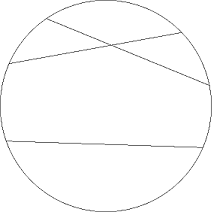
\includegraphics{klein.png}

Эта модель предполагает, что наше пространство на самом деле как бы ограничено, и поэтому в силу именно ограниченности мы можем изобразить какое угодно количество прямых, не пересекающих заданную и проходящих через заданную точку. Единственный сложный вопрос в этой модели в измерении расстояния. При движении к краю окружности масштаб длин должен увеличиваться, чтобы модель удовлетворяла 3 и 4 аксиомам, и одно и то же расстояние в центре диска Клейна и на его краю будет выглядеть сильно по-разному.

Эта модель интересна тем, что она целиком формулируется в терминах геометрии Евклида. То есть модель геометрии Лобачевского получается из непротиворечивости геометрии Евклида: если непротиворечива евклидова геометрия, то непротиворечивой окажется и геометрия Лобачевского, хотя обе они содержат противоречащую друг другу аксиому. Позже выяснилось, что геометрия Лобачевского является не только интересным теоретическим построением но имеет физический смысл: скорости в теории относительности Эйнштейна описываются как раз законами геометрии Лобачевского.

Я к сожалению забыл называние и автора интересной книжки о вымышленном мире, который представлял собой шар в евклидовой геометрии, населенный людьми. Этот шар подчинялся следующему закону: чем ближе человек находился к границе шара, тем меньше он становился по размеру и тем большими для него оказывались расстояния. Эти вымышленные человечки проводили физические эксперименты, и таким образом выяснили, что их вселенная бесконечна и подчиняется законам геометрии Лобачевского. То что на самом деле они живут в евклидовом шаре с особыми свойствами они никаким образом понять не могли.

Как подобный шар и подобные люди могут быть описаны математически мы увидим позже, но сама подобная интерпретация довольно интересна тем, что показывает ограниченность возможности познания: как эти сферические люди ни будут пытаться, они никогда не смогут выяснить что находится за пределами их шара и ничего не узнают о геометрии Евклида, которой на самом деле подчиняется их мир.

Нам же этот пример с геометриями интересен прежде всего тем, что он является хорошей демонстрацией неполноты теории: в абсолютной геометрии утверждение пятой аксиомы является невыводимым, и его можно в результате принять как еще одну аксиому, либо же можно принять как аксиому противоположное утверждение, и оно так же будет непротиворечиво.

Но все сказанное до сих пор относилось лишь к геометрии. Аксиоматизация арифметики натуральных чисел происходила гораздо позднее, чем геометрии, и вплоть до XIX века манипуляции с натуральными числами была неформализованы, и далеко не все видели в такой формализации вообще необходимость. Математик Леопольд Кронекер говорил: «Бог создал натуральные числа, а всё прочее — дело рук человеческих». На сегодняшний день самой известной формализацией (после изложенной мной в этой главе) является система аксиом Пеано, изложенная им в 1889 году в его книге «Принципы арифметики представленные новым методом».

Его аксиомы определяли множество натуральных чисел с помощью константы $0$ и операции инкремента $S$, однако как конкретно выглядят эти константы и операция на языке теории множеств не указывалось, а вместо этого формулировался ряд довольно косвенных свойств, которые были достаточны для определения арифметики:

1) Равенство чисел определялось как отношение эквивалентности.

2) Для любого $n\in\mathbb{N}$ формула $S(n) = 0$ определялась как ложная.

3) $S$ объявлялась инъективной функцией.

4) Оговаривался принцип индукции: если $\phi(0)$ истинно и $\forall n\in\mathbb{N}, \phi(n)\rightarrow \phi(S(n))$, то $\forall n\in\mathbb{N}, \phi(n)$.

Операции сложения и умножения чисел определялись следующим образом:

5) $a+0 = a$

6) $a+S(b) = S(a + b)$

7) $a0 = 0$

8) $aS(b) = ab + a$

Этих аксиом и определений оказывалось достаточным для доказательства всех базовых арифметических свойств.

{\bfseries Упражнение.} Докажите из аксиом Пеано коммутативность умножения $ab=ba$.

Долгое время производились попытки доказать непротиворечивость и полноту аксиом Пеано. Эти попытки были окончательно разбиты в 1931 году, когда Гёдель представил свои теоремы о неполноте. Здесь надо сказать, что Гёдель доказывал теоремы несколько не в том виде и несколько не так, как я представил их в прошлом параграфе. Он был нацелен именно на аксиомы Пеано и использовал в основном аппарат математической логики, а не теории множеств, как это сделал я. Впрочем, у нас не стояло задачи сформулировать максимально строго теорему Гёделя, а лишь понять ее следствия, существенные для большинства математиков.

Для определения натуральных чисел аксиомы Пеано сегодня полностью вытеснены более удобными определениями ZFC. Определение сложения и умножения аксиом Пеано тем не менее осталось довольно полезным, поскольку оно обобщается, и с помощью них  можно удобно определять операции над числами более общего вида, так называемыми ординалами.

ZFC сейчас является базой для 99\% всей существующей математики, хотя детали аксиом и правил вывода чаще всего не используются и большинство математиков с ними не знакомы. Вообще основания математики в виде логики и теории множеств существуют довольно отдельно от остальной математики. Терминология теории множеств используется просто как удобный язык, а из логики математики вообще редко прибегают к чему-либо.

Изначально математическая логика развивалась больше как интересное философское направление, позже она постепенно прилаживалась для формализации аксиоматических систем, с развитием компьютерной техники были надежды, что она может стать основой для искусственного интеллекта, но на деле эти надежды оказались сильно преувеличенными. Сейчас математическая логика живет в значительной степени отдельно от остальной математики и какие-то логические результаты лишь изредка вырываются в мир «большой математики». Пожалуй сколько-нибудь значимыми для широких кругов математиков являются лишь рассмотренные в прошлом параграфе теоремы Гёделя, а так же теорема Лёвенгейма-Скулема, которую мы сможем понять лишь позже. Впрочем, даже эти результаты мало кому известны и используются главным образом не сами они, а их следствия.



\chapter{Натуральные числа}
В этой части наконец-то вводится понятие натурального числа. Основные две темы ~--- само понятие натурального числа (включая минимум из теории чисел) и комбинаторика. Базовые комбинаторные формулы сами по себе часто оказываются полезны в самых разных областях математики, так же на них легко и приятно отрабатывать основные навыки работы с базовыми математическими объектами. В более абстрактные области мы уйдем со следующей главы, эта же глава будет во многом простая, расслабляющая и легкая для чтения (возможно, кроме первого параграфа, который в принципе многим читателям будет необязателен).

\section{Определение}

Натуральные числа~--- это 0, 1, 2, 3, и~т.д. Все это вроде знают. Но как определить понятие натурального числа строго? Чтобы оценить задачу, прежде чем читать дальше, попробуйте дать такое определние самостоятельно, заодно с определение арифметических операций и не опираясь на физическую интуицию, а лишь на логику. Замечу, что этот параграф носит малоприкладной характер~--- его цель лишь в определении натуральных чисел. Я же не могу написать: <<а с этого момента давайте использовать натуральные числа>>. Определить я их обязан как-то, но в то же время подробные определения, которые я здесь привожу, вряд ли будут кому-то действительно полезными. Поэтому данный параграф можно читать наискосок либо не читать вообще, если вы помните свойства натуральных чисел.

Дать строгое опредение пытались многими простыми способами, но все более-менее интуитивные подходы неизменно заводят в тупик. На данный момент мейнстримом в определении натуральных чисел являются два подхода: определение непосредственно на основе теории множеств (определение Фреге-Рассела) и чуть более сложный, но так же важный в силу полезных обобщений, подход на основании аксиом Пеано. Мы не будем рассматривать подробно и формально эти подходы со всеми выкладками, а лишь рассмотрим суть этих определний. Недостающие пробелы вы можете закрыть сами~--- это довольно большая работа, но без каких-либо принципиальных сложностей. Более подробно и обстоятельно мы вернемся к аксиоматизации натуральных чисел позже в шестой главе, когда будем говорить о бесконечных множествах.

Определение Фреге-Рассела отражает идею о том, что натуральные числа отражают количество элементов во множествах. Это довольно понятно на пальцах, но надо дать строгое определение. Первая идея, которая обычно приходит на ум~--- это взять вообще все множества в принципе и разбить их на классы эквивалентности так, чтобы в одном классе оказали множества одинакового размера.

Ввести такую эквивалентность для множеств не сложно: в \S~2.4 мы уже вводили понятие равномощности. В соответствии с тем определением, два множества $A$ и $B$ называются равномощными, если существует некоторая биективная (то есть взаимооднозначаная) функция $f:A\to B$. Пусть например у нас есть множество трех букв алфавита $A=\{a, b, c\}$ и странное множество $B=\{\heartsuit, \clubsuit, \spadesuit\}$. Эти два множества равномощны, так как существует биекция $$f=\{(a, \clubsuit), (b, \heartsuit), (c, \spadesuit)\}$$ --- то есть существует способ назначить каждому элементу множества $A$ некий элемент множества $B$ и обратно. Если мы рассмотрим теперь множество с одним дополнительным элементом $C=\{\heartsuit, \clubsuit, \spadesuit, \Diamond\}$, то увидим, что никаких способов задать тут биекцию не существует, и стало было множество $C$ не равномощно $A$ и $B$.

\begin{exercise}
Докажите, что на любом множестве, состоящим из множеств, отношение биекции~--- это отношение эквивалентности.
\end{exercise}

Теперь, когда у нас есть некое отношение эквивалентности, мы хотим задать классы эквивалентности~--- и эти классы эквивалентности мы могли бы объявить натуральными числами, тогда каждое натуральное число представляло собой класс всех множеств одинаковой мощности. К сожалению, поступить таким образом мы не можем, так как классы эквивалентности могут быть построены лишь на некотором множестве, и в нашем случае было бы необходимым рассматривать множество всех множеств. Последнего, однако, как мы показали в \S~2.5, не существует.

Тем не менее, эта идея всё же может быть доведена до конца, если вместо задания сразу всего класса эквивалентности, мы зададим лишь по одному представителю из этого класса, а затем, чтобы определить принадлежность некоторог множества к классу, мы будем сравнивать это множество с представителями классов. Это похоже на то, что делают в физике при измерениях: вначале определяют некий один эталонный объект (скажем, метр), а затем все остальные сравнения производятся уже относительно него.

Самый маленький класс множеств~--- это пустое множество. Представителем этого класса логично выбрать $\emptyset$. Обозначим его как $$0 = \emptyset$$

Следующим за ним класс должен состоять из только одного элемента. Этим элементом можно взять как раз число 0, и определить представителя нашего нового класса как $$1 = \{0\} = \{\emptyset\}$$

Теперь определим представителя для еще более крупного множества, в котором на один элемент больше. Для этого естественно использовать уже имеющиеся у нас элементы 0 и 1: $$2 = \{0, 1\} = \{\emptyset, \{\emptyset\}\}$$

Ну и до кучи: $$3 = \{0, 1, 2\} = \{\emptyset, \{\emptyset\}, \{\emptyset, \{\emptyset\}\}\}$$

Процедура, в общем-то, проста. Если у нас есть число $n$, то мы можем определить следующий за ним элемент: $$S(n) = n \cup \{n\} = \{0, 1, \ldots, n\}$$

Применяя эту процедуру бесконечное число раз, мы можем получить все натуральные числа. Это на самом деле не столь очевидно, но Infinity Axiom гарантирует нам, что подобным образом действительно возможно определить некое множество, которое мы будем обозначать как $\mathbb{N}$ и называть его множеством натуральных чисел. Теперь мы готовы для наших первых определений.

\begin{definition}
Множеством \term{натуральных чисел} $\mathbb{N}$ называется множество чисел, полученных из $0=\emptyset$ примененением функции $S$.
\end{definition}

\begin{definition}
\term{Последовательностью} элементов множества $X$ называется функция $x:\mathbb{N}\to X$. Обозначается последовательность как $\{x_n\}$.
\end{definition}

\begin{definition}
\term{Конечной последовательностью} элементов множества $X$ называется функция $n \to X$.
\end{definition}

\begin{definition}
Множество $X$ называется \term{конечным}, если существует равномощное ему множество $n\in\mathbb{N}$. В противном случае $X$ называется \term{бесконечным}.
\end{definition}

\begin{definition}
\term{Мощностью} конечного множества $X$ называется такое число $n\in \mathbb{N}$, что $X$ и $n$ равномощны. Обозначается это как $|X| = n$.
\end{definition}

Здесь, вероятно, требуются примеры. Возьмём опять наше множество $C=\{\heartsuit, \clubsuit, \spadesuit, \Diamond\}$. Если без формализма, а на уровне интуиции, то его мощность~--- это количество элементов в нём. Это очевидным образом связано с определением, данным нами выше, если вспомнить, что $4 = \{0, 1, 2, 3\}$. Тогда биекцией $4\to C$, устанавливающей равномощность, может быть функция $f = \{(0, \heartsuit), (1, \clubsuit), (2, \spadesuit), (3, \Diamond)\}$. Аналогичным образом получается связь и других определений с нашей интуицией~--- здесь может быть непривычным лишь то, что мы рассматриваем натуральные числа как множества, но именно это, если вдуматься, позволяет нам устанавливать между ними и множествами соответствия, используя привычный механизм функций.

\begin{definition}
Мы говорим, что число $m$ \term{меньше или равно} $n$ и обозначаем это как $m\le n$, если $m\subset n$.
\end{definition}

\begin{definition}
Мы говорим, что число $m$ \term{меньше} $n$ и обозначаем это как $m<n$, если $m< n$ и $m \not= n$.
\end{definition}

\begin{thm}
Отношение $\le$ задаёт линейный порядок на $\mathbb{N}$.
\end{thm}
\begin{proof}В качестве упражнения.\end{proof}

\begin{thm}
$S(n) > n$ для любого $n$.
\end{thm}
\begin{proof}
Элементарно.
\end{proof}

\begin{example}
Сравним числа 3 и 4. Мы знаем, что $3 = \{0, 1, 2\}$ и $4 = \{0, 1, 2, 3\}$. Очевидно, что $3\subset 4$, и, следовательно, $3\le4$. Поскольку $3\not= 4$, то $3<4$.
\end{example}

В полной аналогии с приведенными определениями можно определить так же сравнения \term{больше} ($>$) и \term{больше или равно} ($\ge$).

\begin{thm}
Множество $\mathbb{N}$~--- бесконечное.
\end{thm}
\begin{proof}
Пусть $\mathbb{N}$ конечно и $n = \max\{\mathbb{N}\}$. Тогда $m = |\mathbb{N}| = S(n) > n$, но поскольку $n$~--- максимальный элемент, $m\not\in\mathbb{N}$, что противоречит определению $\mathbb{N}$. Что и требовалось доказать.
\end{proof}

На самом деле для порядка натуральных чисел справедливо даже более сильно утверждение, к которому мы будем обращаться время от времени, а потом подробнее рассмотрим его в шестой главе:

\begin{definition}
Множество называется вполне упорядоченным, если любое его подмножество имеет минимальный элемент.
\end{definition}

\begin{thm}
Множество $\mathbb{N}$ вполне упорядочено относительно порядка $\le$.
\end{thm}
\begin{proof}
В качестве упражнения.
\end{proof}

Теперь немного отвлечемся от подхода Фреге-Рассела и посмотрим на аксиомы Пеано. Эти аксиомы не отвечают на вопрос что же вообще такое натруальные числа, но постулируют существование некоего множества $\mathbb{N}$ такого, что в нем существует выделенный элемент 0, и на котором задана некая инъективная функция $S:\mathbb{N}\to\mathbb{N}$ такая, что любой элемент $\mathbb{N}$ кроме 0 имеет обратный. Это не совсем полная аксиоматика~--- мы будем её дополнять по мере надобности, но уже сейчас очевидно, что это определение практически дублирует подход Фреге-Рассела за исключением того, что мы не определяем конкретный вид элементов множества $\mathbb{N}$, но этого, на самом деле вполне достаточно~--- этим определением можно пользоваться, хотя жизнь при этом получается намного сложнее, как мы увидим ниже.

Перейдём теперь к определению арифметических операций. Вначале я буду давать интуитивное определение, затем доводить его до строгого вида в аксиоматике Фреге-Рассела, и затем определение для аксиом Пеано.

\begin{definition}
Пусть у нас есть непересекающие множества $M$ и $N$, такие что $|M|=m$ и $|N| = n$. Будем писать, что $|M\cup N| = m+n$, а число $m+n$ называть \term{суммой} $m$ и $n$.
\end{definition}

Это имеет очень простой комбинаторный смысл: если у нас есть некоторый набор, состоящий из $n$ объектов и мы его объединяем с набором, состоящим из $m$ объектов, то в результате мы получим набор, состоящий из $n+m$ объектов. Это то что объясняют в первом классе школы, но только более абстрактно.

Тем не менее, это не слишком хорошее определение. Во-первых, оно даёт нам понятие суммы не в терминах самих чисел, а в терминах неких множеств, причем непересекающихся. Это плохо, поскольку сами числа, будучи множествами, всегда пересекаются друг с другом (кроме числа 0). Поэтому если у нас есть два числа, не привязанных к конкретным множествам, это определение не даёт нам понять как определить их сумму.

Во-вторых, встаёт такой неприятный вопрос: пусть у нас есть непересекающиеся множества $A$ и $B$, такие что $|A|=|N|$ и $|B|=|N|$, можем ли мы в этом случае гарантировать, что $|A\cup B| = |N\cup M|$? Интуитивно это очевидно, но как это доказать~---вопрос нетривиальный.

И в третьих, всё еще хуже: даже если $A$ и $B$ конечны, то где гарантия, что их объединение будет так же конечным? Опять же, это очевидно, но поди докажи (а когда мы будем говорить о бесконечных множествах, выяснится, что подобные очевидные рассужения часто банально неверны).

Первая проблема утраняется c помощью следующих двух упражнений:

\begin{exercise}
Докажите, что $|m\times 1| = m$ для $m\in\mathbb{N}$.
\end{exercise}

\begin{exercise}
Докажите, что $(m\times 1) \cap m = \emptyset$.
\end{exercise}

Пользуясь этими двумя утверждениями, можно ввести такое определение:

\begin{definition}
$m + n = |m\times1 \cup n|$.
\end{definition}

Это решает первую и вторую (после некоторых несложных раздумий) обозначенную нами проблему, но не решает третью. Её можно решить либо с помощью метода матиндукции, который мы отложим на последующие параграфы, либо используя изначально более абстрактные конструкции и обобщая натуральные числа на случай бесконечных множеств, что мы оставим до шестой главы нашего учебника для начинающих.

А теперь то же самое определение, но уже в аксиоматике Пеано:

\begin{definition}
Сложение определяется следующим образом:\\*
n + 0 = n\\*
n + S(m) = S(m + n)
\end{definition}

\begin{example}
$$n + 3 = n + S(2) = S(n+2) = S(n+2)
=S(n+S(1)) = S(S(n+1)) = S(S(S(n)))$$
\end{example}

Как видно из примера, это определение фактически говорит, что выражение $m + n$ означает, что к числу $m$ применяется операция $S$ (фактически, увеличение на единицу), $n$ раз. Интуитивно это должно буть понятно, строгое же доказательство того, что такое определение правомочно, будет дано позже.

\begin{thm}
Справедливы следующие свойства сложения:
\begin{enumerate}
\item нейтральность нуля: $a + 0 = a$
\item коммутативность: $a + b = b + a$,
\item ассоциативность: $a + (b + c) = (a + b) + c = a + b + c$
\item если $a < b$, то $a + c < b + c$
\end{enumerate}
\end{thm}
\begin{proof}
Нейтральность нуля очевидна. Для коммутативности и ассоциативности используя определение Фреге-Рассела довольно легко построить биекцию между левыми и правыми частями равенства. Последнее равенство следует из того, что если $a < b$, то $S(a) < S(b)$ (доказывается элементарно), а прибавление любого натурального числа равносильно многократному применению операции $S$. Используя только аксиоматику Пеано это можно доказать, опять же, по индукции, о чем будет отдельный параграф.
\end{proof}

Пользуясь сложением легко определить линейный порядок на $\mathbb{N}$ в случае аксиом Пеано (для Фреге-Рассела это будет элементарная теорема):

\begin{definition}
$a < b$, если существует такое $n$, что $a + n = b$.
\end{definition}

\begin{definition}
Операция вычитания: мы пишем $a = b - c$, если $a + c = b$. В этом случае $a$ называется \term{разностью} $b$ и $c$.
\end{definition}

\begin{thm}
Операция $a - b$ определена только в том случае, если $a \ge b$.
\end{thm}
\begin{proof}В качестве упражнения\end{proof}

\begin{definition}
Операция умножения для Фреге-Рассела: $ab = |a\times b|$
\end{definition}

Здесь опять же надо внимательно отнестись к тем комментариям, которые я приводил для сложения, я на этом уже не буду подробно останавливаться.

Если смотерть на умножение комбинаторно, то получается простая интерпретация: для произвольных множеств $A$ и $B$ с мощностями $a$ и $b$ соответственно, имеем $|A\times B| = ab$. То есть произведение чисел~--- это количество элементов в декартовом произведении множеств соответствующих размеров. Это очень часто используется в самой базовой комбинаторике, например, так:

\begin{exercise}
Пусть у нас есть три бабы и два мужика. Сколько гетеросексуальных пар из них можно составить?
\end{exercise}

\begin{definition}
Операция умножения для аксиом Пеано:\newline
\item $m\cdot 0 = 0$\newline
\item $m\cdot S(n) = mn + m$
\end{definition}

\begin{thm}
Справедливы следующие свойства:
\begin{enumerate}
\item $0\cdot a = 0$
\item нейтральность единицы: $1\cdot a = a$
\item коммутативность: $ab = ba$
\item ассоциативность: $a(bc) = (ab)c = abc$
\item дистрибутивность: $a(b+c) = ab + ac$
\item если $a < b$ и $c \not= 0$, то $ac < bc$
\end{enumerate}
\end{thm}
\begin{proof}
Здесь всё аналогично доказательству подобных свойств для сложения~--- необходимо просто построить биекцию для левой и правой части (причем это не так просто, если ударяться прямо в формализм ZFC, хотя и возможно по индукции). Рекомендую самостоятельно попытаться строго проработать случай коммутативности, поскольку он не сложен, но далеко не все понимают её для умножения.

Если отойти от формализма и посмотреть на вопрос геометрически, то $mn$ можно рассматривать как количество ячеек в таблице с $m$ строками и $n$ столбцами, а $nm$~--- количество ячеек в той же таблице, поставленной на бок~--- в этом случае строки и столбцы меняются местами, но количество ячеек при этом не меняется.

Из этой табличной интерпретации можно уже построить конкретную биекцию. Как увязываются таблицы и декартовы произведения рассматривалось в \S~2.2. Остальные приведенные здесь свойства могут быть интуитивно мотивированы подобным же образом.
\end{proof}

Используя обозначение $S(n) = n+1$ и свойство дистрибутивности можно легко понять смысл определния умножения в аксиомах Пеано: $mS(n) = m(n+1) = mn + m$.

\begin{thm}
Для любых $a$ и $b$ найдутся такие числа $r<b$ и $q$, что $a = qb + r$.
\end{thm}
\begin{proof}
Будем строить конечную последовательность $\{r_n\}$ следующим образом: $r_n = a - nb$ для тех значений $n$, для которых вычитание будет определено. Множество элементов этой последовательсноти имеет минимальный элемент, который мы и обозначим как $r = a - qb$. Это и есть утверждение теоремы.
\end{proof}

\begin{definition}
Пусть $a = qb + r$. $q$ называется \term{частным от деления} $a$ на $b$, а $r$ \term{остатком от деления}.
\end{definition}

\begin{definition}
Если остаток от деления $a$ на $b$ равен нулю, то говорят, что $a$ \term{делится} на $b$, или что $b$ \term{делит} $a$. Обозначается это как $a\vdots b$ и  $b|a$ соответственно, а частное в этом случае обозначается как $a\over b$.
\end{definition}

\begin{exercise}
Докажите, что отношение делимости задаёт частичный порядок на $\mathbb{N}$.
\end{exercise}

\begin{definition}
Возведение в стемень для Фреге-Рассела: пусть $m = |M|$ и $n = |N|$, тогда $m^n = |M^N|$
\end{definition}

Напомню, что $M^N = \{f|f:N\to M\}$~--- то есть это множество функций из $N$ в $M$. Это имеет простой комбинаторный смысл. Пусть, например, $M$~--- множество цветов рубашек и $N$~-- множество мужчин. Каждый мужчина выбирает себе цвет рубашки. Если все мужчины сделали свой выбор, то этот выбор представляется функцией $f: N \to M$. Сколько всего есть вариантов выбора цветов для всех мужчин сразу? Ровно столько, сколько есть таких функций, то есть ровно столько, какова мощность множества $M^N$. Остаётся только вопрос в том, как посчитать эту величину.

\begin{exercise}
Пусть для кодирования мы используем символы $\{a, b, c, d\}$. Сколько существует различных кодовых слов длины 5?
\end{exercise}

\begin{thm}
$m^n = \underbrace{m\cdot m \cdot \ldots \cdot m}_n$
\end{thm}
\begin{proof}
Пусть $|M| = m$ и $|N| = n$. Я приведу не самые строгие рассуждения, строго это опять же надо доказывать по индукции. Возьмём некоторый элемент $N$. Он может быть отображен в один из элементов $M$, которых $n$ штук. Возьмём другой элемент $N$, он так же может быть отражен на один из $n$ элементов $N$. Итого для первых двух элементов $N$ существует $m\cdot m$ вариантов отображения. Если теперь рассмотреть еще один элемент $N$, то он так же может быть отображен в $m$ элементов, итого вариантов для отображения первых трех элементов оказывается равно $m\cdot m\cdot m$. Продолжая рассуждения мы получим утверждение теоремы, поскольку в множестве $N$ всего $n$ элементов.
\end{proof}

Приведенное рассуждение подсказывает нам как можно определить степень для аксиоматики Пеано:

\begin{definition}
Степень в аксиоматике Пеано:\newline
$a^0 = 1$\newline
$a^{S(n)} = a^na$
\end{definition}

\begin{thm}
Для степеней справедливы следующие свойства:
\begin{enumerate}
\item $a^0 = 1$
\item $a^b a^c = a^{b+c}$
\item $(a^b)^c = a^{bc}$
\item если $a > b$, то для любого $c > 0$, $a^c > b^c$
\item если $a > b$, то для любого $c > 1$, $c^a > c^b$
\end{enumerate}
\end{thm}
\begin{proof}
Первое свойство дублирует определение Пеано, но его можно увидеть и из определения Фреге-Рассела: существует всего лишь одна функция из пустого множества в некоторое другое, и эта функция сама является пустым множеством. Функция вида $f:\emptyset\to X$ совершенно легальна и единственна, хоть она ничего и не отображает.

Второе свойство: $a^ba^c = \underbrace{\underbrace{a\cdot\ldots\cdot a}_b \cdot \underbrace{a \cdot\ldots \cdot a}_c}_{b+c} = a^{b+c}$

Третье свойство: $(a^b)^c = \underbrace{a^ba^b\ldots a^b}_c = a^{bc}$

Оставшиеся свойсва предлагаю доказать самостоятельно в качестве упражнения.
\end{proof}

Приведенное определение Фрегге-Рассела может почти сразу дать нам ответ на вопрос о том сколько всего подмножеств имеет некоторое множество, а заодно объяснить обозначение $2^X$ для булеана. Прежде, однако, нам понадобится одно вспомогательное понятие.

\begin{definition}
Пусть $X\subset U$. Функция $\chi_X: U\to \{0,1\} = 2$ называется \term{индикаторной функцией} множества $X$, если $\chi_X(t) = 1$ при $t\in X$ и $\chi_X(t) = 0$ в противном случае.
\end{definition}

Каждому подмножеству $U$ соответствует своя характеристическая функция, ровно как и характеристической функции соотстветствует подмножество. Это соответствие позволяет нам легко получить желаемую теорему:

\begin{thm}
$|2^X| = 2^{|X|}$
\end{thm}
\begin{proof}
Для того, чтобы определить количество элементов в булеане, нам достаточно определить количество различных характеристических функцих на множестве $X$. Поскольку характеристическая функция имеет вид $\chi:X\to 2$, множеством всех таких функций является $2^X$. По теореме 3.9 мощность этого множества $2^{|X|}$
\end{proof}
\section{Позиционные системы счисления}

После того как мы определили понятие натурального числа, встаёт вопрос о том, как натуральные числа записывать. Пока мы ввели только символы 0, 1, 2, 3 и 4 для нескольких чисел. Мы могли бы продолжить процесс и дальше (пока продолжим этот ряд последовательно символами 5, 6, 7, 8, 9, A), однако довольно быстро возникает проблема: множество $\mathbb{N}$ бесконечное, и соответственно символов нам потребуется бесконечно много, что, видимо, невозможно. Нам нужен способ, который позволит записывать любое натуральные число используя конечное число символов.

Пусть у нас есть некоторое число $n$, которое надо записать. Выберем некоторое произвольное $b > 0$, которое будем называть основанием нашей системы счисления и поделим одно на другое с остатком:
\begin{equation}\label{eq:n0}
n = q_0b + r_0
\end{equation}
Здесь $r_0 < b$ и $q_0 < n$. Поделим теперь на $b$ с остатком значение $q_0$: $$q_0 = q_1b + r_1$$ и подставим это выражение в \eqref{eq:n0}:
\begin{equation}\label{eq:n1}
n = (q_1b + r_1)b + r_0 = q_1b^2 + r_1b + r_0
\end{equation}

Аналогично можно представить $q_1 = q_2b + r_2$ подставив его в \eqref{eq:n1}, затем $q_2$, $q_3$ и так далее. Легко увидеть, что последовательность $\{q_i\}$ с каждым следующим элементом убывает, и, стало быть, в какой-то момент найдётся такое $k$, что $q_k = 0$. На этом процесс прекратится и мы получим такое выражение для $n$:
\begin{equation}\label{eq:nk}
n = r_kb^k + r_{k-1}b^{k-1} +\ldots + r_1b + r_0
\end{equation}

В этом выражении важно то, что каждое из значений $r_i$ оказывается меньше чем $b$, и при этом набора $\{r_i\}$ вполне достаточно для того, чтобы однозначно идентифицировать любое число. В этом и заключается основная идея позиционных систем счисления. Число $b$ определяет количество символов, необходимых для представления числа в системе с основанием $b$.

В компьютерах применяется так называемая двоичная система счисления, в которой $b=2$ и используются лишь два символа для записи чисел: 0 и 1. Это обуслевлено тем, что на физическом уровне в вычислительных системах довольно просто отличить два принцпиально различных состояния друг от друга: есть напряжение в проводе/нет напряжения, луч отражается от диска под большим углом/под маленьким, сектор на диске намагничен/ненамагничен. И так далее. Возможно, конечно, и более детальное различение физичеких систем, например мы могли бы различать не просто наличие напряжения, но и его величину: слабое оно или сильное в дополнение к тому, если ли оно вообще. В этом случае $b$ было бы равно трём, и иногда это действительно используется, но технически это часто осуществляется сложнее, поэтому почти всегда используется $b=2$.

Рассмотрим пример. Как представить число $A$ в двоичной системе? (Напомню, что за $A$ мы обозначили число, следующее за числом 9). Проделывая процедуру с делением, описанную в начале параграфа, мы приходим к записи
$$A = 1\cdot 2^3 + 0\cdot 2^2 + 1\cdot 2 + 0$$
Здесь $r_3 = 1, r_2 = 0, r_1 = 1, r_0 = 0$. Можно кратко записать это как упорядоченный набор: $(1, 0, 1, 0)$, или же даже еще короче, опустив скобки и запятые: 1010. Это и есть двоичное представления числа A. Чтобы не путать системы счисления, удобно так же обозначать основание рядом с числом. В нашем случае получится $1010_2$. Впрочем, иногда нам будет удобно пользоваться и записью $(1, 0, 1, 0)_2$, так что следует иметь её ввиду, по крайней мере в течение ближайших нескольких параграфов. Количество символов, необходимых для представления числа, мы будем называть разрядностью, а выражение $r_ib^i$ $i$-ым разрядом. Иногда нам будет удобно считать, что число имеет больше разрядов чем необходимо, тогда старшие разряды будут иметь значение 0. Таким образом число $1010_2$ можно было бы эквивалентно записать как $00001010_2$. Потенциально мы можем считать, что слева в записи числа стоит бесконечное число нулей~--- это соображение часто упрощает рассуждения и мы будем пользоваться им ниже.

В повседневной жизни чаще всего применяется десятичная система счисления, в которой $b=A$ и помимо 0 и 1 используются так же символы 2, 3, 4, 5, 6, 7, 8, 9. Рассмотрим, для примера, как представить число $10011001_2$ в десятичной системе счисления. Повторяя еще раз процедуру деления с остатком, получаем:
$$10011001_2 = 1\cdot A^2 + 5\cdot A + 3 = 153_A$$

Рассматривая этот пример, у вас могут возникнуть сомнения по поводу того, как я это вычислил. Ответ тут очень простой: я использовал инженерный калькулятор, который умеет работать с разными системами счисления. Впрочем, даже без калькулятора можно было бы удостовериться в верности данного выражения. Самый простой способ поделить $a$ на $b$ с остатком заключается в многократном вычитании $b$ из $a$ до тех пор, пока результат не окажется меньше $b$. Этот способ легко понять, но он крайне неэффективен: для его реализации вам потребуется уже не калькулятор, а полноценный компьютер. Тем не менее вычислить это возможно. Пока мы остановимся на этом способе и на самом факте того, что это можно как-то вычислить, а в следующем параграфе я продемонстрирую более эффективный способ деления с остатком, который позволит провести все вычисления используя лишь ручку и клочек бумажки.

Вездее далее, если не будет оговорено обратное, мы будем использовать десятичную систему счисления, при этом обозначать её мы не будем никак специально, то есть вместо $123_{10}$ мы будем ограничиваться записью $123$.

В качестве последнего примера рассмотрим шестнадцатеричную систему счисления ($b=16$), часто используемую программистами. В ней помимо символов десятичной системы применяются так же символы $A, B, C, D, E, F$. Рассмотрим пример того, как можно понять десятичное значение числа в шестнадцатеричной записи:
$$ABF_{16} = A\cdot 16^2 + B\cdot 16 + F = 10\cdot 256 + 11 \cdot + 15 = 2751$$

Причина, по которой программисты любят шестнадцатеричную систему счисления, заключается в том, что она очень легко переводится в двоичную систему счисления и обратно. По сути для этого надо знать лишь представление в двоичной системе 16-ти цифр. Для примера выше мы уже видели, что $A_{16} = 1010_2$, так же легко увидеть, что $B_{16} = 1011_2$ и $F_{16} = 1111_2$. Чтобы получить отсюда двоичную запись, достаточно объединить двоичные записи для отдельных шестнадцатеричных цифр: $$ABF_{16} = 1010\:1011\:1111_2$$

Возможность такого представления основывается на следующей несложной общей теореме (сложнее понять формулировку, чем доказать), доказательство которой мы оставим в качестве упражнения читателю (впрочем, я бы пока рекомендовал отложить это упражнение и вернуться к нему после прочтения следующего параграфа):
\begin{thm}
Записи в системах счисления с основаниями $b$ и $c = b^k$ связаны следующим образом: $$(d_{kn},\dots, d_0)_b = ((d_{kn}, \ldots, d_{(k-1)n + 1})_b, \dots, (d_{2k}, \dots, d_{k+1})_b , (d_k, \dots, d_0)_b)_c$$
\end{thm}

В компьютерной памяти чаще всего двоичные значения 0 и 1 (их называют битами) объединены в группы по восемь бит (число восемь берется из соображений, близких к только что упомянутой теореме). Такая группа бит называется байтом. Во многих системах один байт представляет собой один печатный символ. Если же рассматривать байт как число, что его значения могут варьироваться от 0 до 255 (всего 256 различных значений), и таким образом каждому символу можно сопоставить некоторое числовое значение. Всего у нас может быть максимум 256 символов.

Если рассматривать не один, а сразу последовательность байт, то их можно считать числом, записанном в 256-ричной системе счисления. Это часто применяется в компьютерах для записи больших чисел. Если рассматривать два байта, то их максимальным значением может быть 65535. Если считать за символ не один байт, а два байта, то это значит, что наша система сможет поддерживать 65535 символов, что хватит даже китайцам с несколькими их диалектам, Египтянам, латинянам и евреям. Если нам и этого мало, то можно рассматривать четырехбайные значения. В этом случае мы сможем записать число 4294967295, то есть четыре байта позволяют записывать девятизначные числа и некоторые десятизначные. С точки зрения символов мы сможем уместить сюда не только все распространенные в мире языки, но и все вымершие языки, смайлики, музыкальные обозначения, матемаетические знаки, несколько вариантов древней клинописи и так далее. Если нам и этого не хватит, то можно взять 8-байтные целые, которые позволят работать с 19-значными числами.

Если мы будет рассматривать текст как последовательность символов, то мы так же эту последовательность можем интерпретировать как некоторое большое число. Например, для кодирования английского текста чаще всего применяется стандарт ASCII, устанавливающий какой букве соответствует какое число. Букве F в нём соответствует число 70, а букве o~--- 111 (ASCII использует только 1 байт для кодирования символов). Как число слово Foo в ASCII можно представить следующим образом:
$$Foo = 70 \cdot 256^2 + 111 \cdot 256 + 111 = 4587520 + 28416 + 111 = 4616047$$

Подобное отношение к тексту позволяет применять к нему математические функции. Например, многие криптосистемы представляют собой лишь некоторые арифметические действия над числами и даже не догадываются о том, что пользователь рассматривает данные как текст. Самым ярким примером является криптосистема RSA, на которой сейчас построена значительная доля всей криптографии, используемой на практике, и которую мы рассмотрим в четвертой главе. Используя действия над числами можно так же сжимать данные, чтобы они занимали меньше места. Этот подход называется арифметическим кодированием и мы так же рассмотрим его в четвертой главе. В четвертом параграфе этой главы мы будем рассматривать математические формулы как обычный текст, который в свою очередь мы будем рассматривать как обычное число. Довольно неожиданным образом это позволит сделать нам важные фундаментальные выводы относительно всей математики в целом.




\end{document}
